% Формат А4, 14pt (ГОСТ Р 7.0.11-2011, 5.3.6)
\documentclass[a4paper,14pt]{extreport}

%%%%%%%%%%%%%%%%%%%%%%%%%%%%%%%%%%%%%%%%%%%%%%%%%%%%%%
%%%% Файл упрощённых настроек шаблона диссертации %%%%
%%%%%%%%%%%%%%%%%%%%%%%%%%%%%%%%%%%%%%%%%%%%%%%%%%%%%%

%%%        Подключение пакетов                 %%%
\usepackage{ifthen}                 % добавляет ifthenelse
%%% Инициализирование переменных, не трогать!  %%%
\newcounter{intvl}
\newcounter{otstup}
\newcounter{contnum}
\newcounter{pgnum}
\newcounter{bibliosel}
\newcounter{chapstyle}
\newcounter{headingdelim}
\newcounter{headingalign}
\newcounter{headingsize}
%%%%%%%%%%%%%%%%%%%%%%%%%%%%%%%%%%%%%%%%%%%%%%%%%%

%%% Область упрощённого управления оформлением %%%

%% Интервал между заголовками и между заголовком и текстом
% Заголовки отделяют от текста сверху и снизу тремя интервалами (ГОСТ Р 7.0.11-2011, 5.3.5)
\setcounter{intvl}{3}               % Коэффициент кратности к размеру шрифта

%% Отступы у заголовков в тексте
\setcounter{otstup}{0}              % 0 --- без отступа; 1 --- абзацный отступ

%% Нумерация формул, таблиц и рисунков
\setcounter{contnum}{0}             % 0 --- пораздельно (во введении подряд, без номера раздела); 1 --- сквозная нумерация по всей диссертации

%% Оглавление
\setcounter{pgnum}{1}               % 0 --- номера страниц никак не обозначены; 1 --- Стр. над номерами страниц (дважды компилировать после изменения)

%% Библиография
\setcounter{bibliosel}{0}           % 0 --- встроенная реализация с загрузкой файла через движок bibtex8; 1 --- реализация пакетом biblatex через движок biber

%% Текст и форматирование заголовков
\setcounter{chapstyle}{1}           % 0 --- разделы только под номером; 1 --- разделы с названием "Глава" перед номером
\setcounter{headingdelim}{1}        % 0 --- номер отделен пропуском в 1em или \quad; 1 --- номера разделов и приложений отделены точкой с пробелом, подразделы пропуском без точки; 2 --- номера разделов, подразделов и приложений отделены точкой с пробелом.

%% Выравнивание заголовков в тексте
\setcounter{headingalign}{0}        % 0 --- по центру; 1 --- по левому краю

%% Размеры заголовков в тексте
\setcounter{headingsize}{0}         % 0 --- по ГОСТ, все всегда 14 пт; 1 --- пропорционально изменяющийся размер в зависимости от базового шрифта
               % Упрощённые настройки шаблона 

%%% Проверка используемого TeX-движка %%%
\usepackage{iftex}
\newif\ifxetexorluatex   % определяем новый условный оператор (http://tex.stackexchange.com/a/47579/79756)
\ifXeTeX
    \xetexorluatextrue
\else
    \ifLuaTeX
        \xetexorluatextrue
    \else
        \xetexorluatexfalse
    \fi
\fi

\usepackage{amsmath}
\usepackage{amssymb}
\usepackage{graphicx}
\usepackage{epstopdf}
\usepackage{tabularx}
\usepackage{soul}
\DeclareMathOperator{\sinc}{sinc}
%%% Поля и разметка страницы %%%
\usepackage{pdflscape}                              % Для включения альбомных страниц
\usepackage{geometry}                               % Для последующего задания полей
\usepackage{enumerate}
%%% Математические пакеты %%%
\usepackage{amsthm,amsfonts,amsmath,amssymb,amscd}  % Математические дополнения от AMS
\usepackage{mathtools}                              % Добавляет окружение multlined

%%%% Установки для размера шрифта 14 pt %%%%
%% Формирование переменных и констант для сравнения (один раз для всех подключаемых файлов)%%
%% должно располагаться до вызова пакета fontspec или polyglossia, потому что они сбивают его работу
\newlength{\curtextsize}
\newlength{\bigtextsize}
\setlength{\bigtextsize}{13.9pt}

\makeatletter
%\show\f@size                                       % неплохо для отслеживания, но вызывает стопорение процесса, если документ компилируется без команды  -interaction=nonstopmode 
\setlength{\curtextsize}{\f@size pt}
\makeatother

%%% Кодировки и шрифты %%%
\ifxetexorluatex
    \usepackage{polyglossia}                        % Поддержка многоязычности (fontspec подгружается автоматически)
\else
    \RequirePDFTeX                                  % tests for PDFTEX use and throws an error if a different engine is being used
    \usepackage{cmap}                               % Улучшенный поиск русских слов в полученном pdf-файле
    \usepackage[T2A]{fontenc}                       % Поддержка русских букв
    \usepackage[utf8]{inputenc}                     % Кодировка utf8
    \usepackage[english, russian]{babel}            % Языки: русский, английский
    \IfFileExists{pscyr.sty}{\usepackage{pscyr}}{}  % Красивые русские шрифты
\fi

%%% Оформление абзацев %%%
\usepackage{indentfirst}                            % Красная строка

%%% Цвета %%%
\usepackage[dvipsnames,usenames]{color}
\usepackage{colortbl}

%%% Таблицы %%%
\usepackage{longtable}                              % Длинные таблицы
\usepackage{multirow,makecell,array}                % Улучшенное форматирование таблиц
\usepackage{booktabs}                               % Возможность оформления таблиц в классическом книжном стиле (при правильном использовании не противоречит ГОСТ)

%%% Общее форматирование
\usepackage{soulutf8}                               % Поддержка переносоустойчивых подчёркиваний и зачёркиваний
\usepackage{icomma}                                 % Запятая в десятичных дробях


%%% Гиперссылки %%%
\usepackage{hyperref}

%%% Изображения %%%
\usepackage{graphicx}                               % Подключаем пакет работы с графикой

%%% Списки %%%
\usepackage{enumitem}

%%% Подписи %%%
\usepackage{caption}                                % Для управления подписями (рисунков и таблиц) % Может управлять номерами рисунков и таблиц с caption %Иногда может управлять заголовками в списках рисунков и таблиц
\usepackage{subcaption}                             % Работа с подрисунками и подобным

%%% Интервалы %%%
\usepackage[onehalfspacing]{setspace}               % Опция запуска пакета правит не только интервалы в обычном тексте, но и формульные

%%% Счётчики %%%
\usepackage[figure,table]{totalcount}               % Счётчик рисунков и таблиц
\usepackage{totcount}                               % Пакет создания счётчиков на основе последнего номера подсчитываемого элемента (может требовать дважды компилировать документ)
\usepackage{totpages}                               % Счётчик страниц, совместимый с hyperref (ссылается на номер последней страницы). Желательно ставить последним пакетом в преамбуле

  % Пакеты общие для диссертации и автореферата
%%% Колонтитулы %%%
\usepackage{fancyhdr}

%%% Прикладные пакеты %%% 
\usepackage{calc}               % Пакет для расчётов параметров, например длины
%\usepackage{etoolbox}          % ради функции patchcmd для управления списком литературы

\usepackage {interfaces-base}   % Набор базовых интерфейсов к некоторым пакетам, конкретные реализации загружаются в стиле

%%% Заголовки %%%
\usepackage{titlesec}           % Пакет настройки шрифтов заголовков в тексте

%%% Оглавление %%%
\usepackage{tocloft}

%%% Счётчики %%%
\usepackage{chngcntr}           % оперативная перенастройка счётчиков         % Пакеты для диссертации
\usepackage{tabularx,tabulary}  %таблицы с автоматически подбирающейся шириной столбцов

% Листинги с исходным кодом программ
\usepackage{fancyvrb}
\usepackage{listings}

% Плавающие окружения. во многом лучше пакета float
\usepackage{floatrow}
%Диаграммы Фейнмана
\usepackage{tikz}
\usetikzlibrary{trees}
\usetikzlibrary{decorations.pathmorphing}
\usetikzlibrary{decorations.markings}
\usetikzlibrary{positioning, automata, arrows, arrows.meta}

\usepackage{longtable} %Длинные таблицы
\usepackage{pdfpages}   %Вставлять пдф
\usepackage{afterpage} %Пустая страница
\usepackage{anyfontsize}
        % Пакеты для специфических пользовательских задач
%%% Переопределение именований, чтобы можно было и в преамбуле использовать %%%
\renewcommand{\chaptername}{Глава}
\renewcommand{\appendixname}{Приложение} % (ГОСТ Р 7.0.11-2011, 5.7)
\newcommand\DoubleLine[5][3pt]{%
  \path(#2)--(#3)coordinate[at start](h1)coordinate[at end](h2);
  \draw[#4]($(h1)!#1!90:(h2)$)--($(h2)!#1!-90:(h1)$);
  \draw[#5]($(h1)!#1!-90:(h2)$)--($(h2)!#1!90:(h1)$);
}       % Переопределение именований, чтобы можно было и в преамбуле использовать
%%% Макет страницы %%%
% Выставляем значения полей (ГОСТ 7.0.11-2011, 5.3.7)
\geometry{a4paper,top=2cm,bottom=2cm,left=3cm,right=2cm}

%%% Кодировки и шрифты %%%
\ifxetexorluatex
    \setmainlanguage[babelshorthands=true]{russian}  % Язык по-умолчанию русский с поддержкой приятных команд пакета babel
    \setotherlanguage{english}                       % Дополнительный язык = английский (в американской вариации по-умолчанию)
    \ifXeTeX
        \defaultfontfeatures{Ligatures=TeX,Mapping=tex-text}
    \else
        \defaultfontfeatures{Ligatures=TeX}
    \fi
    \setmainfont{Times New Roman}
    \newfontfamily\cyrillicfont{Times New Roman}
    \setsansfont{Arial}
    \newfontfamily\cyrillicfontsf{Arial}
    \setmonofont{Courier New}
    \newfontfamily\cyrillicfonttt{Courier New}
\else
    \IfFileExists{pscyr.sty}{\renewcommand{\rmdefault}{ftm}}{}
\fi

%%% Интервалы %%%
%linespread-реализация ближе к реализации полуторного интервала в ворде.
%setspace реализация заточена под шрифты 10, 11, 12pt, под остальные кегли хуже, но всё же ближе к типографской классике. 
%\linespread{1.3}                    % Полуторный интервал (ГОСТ Р 7.0.11-2011, 5.3.6)

%%% Выравнивание и переносы %%%
\sloppy                             % Избавляемся от переполнений
\clubpenalty=10000                  % Запрещаем разрыв страницы после первой строки абзаца
\widowpenalty=10000                 % Запрещаем разрыв страницы после последней строки абзаца

%%% Изображения %%%
\graphicspath{{images/}}            % Пути к изображениям

%%% Подписи %%%
\captionsetup{%
singlelinecheck=off,                % Многострочные подписи, например у таблиц
skip=2pt,                           % Вертикальная отбивка между подписью и содержимым рисунка или таблицы определяется ключом
justification=centering,            % Центрирование подписей, заданных командой \caption
}

%%% Рисунки %%%
\DeclareCaptionLabelSeparator*{emdash}{~--- }             % (ГОСТ 2.105, 4.3.1)
\captionsetup[figure]{labelsep=emdash,font=onehalfspacing,position=bottom}

%%% Таблицы %%%
\DeclareCaptionFormat{tablecaption}{\raggedleft #1#2\\%   % Идентификатор таблицы справа, на отдельной строке
    \centering{#3}}                                       % Наименование таблицы строкой ниже и центрировано, без переносов
\DeclareCaptionFormat{tablenocaption}{\raggedleft #1#2%   % Идентификатор таблицы справа, на отдельной строке
}                                                         % Наименование таблицы отсутствует
\captionsetup[table]{format=tablecaption,labelsep=space,singlelinecheck=off,font=onehalfspacing,position=top}  % пробельный разделитель идентификатора с номером от наименования, многострочные наименования и прочее
\DeclareCaptionLabelFormat{continued}{Продолжение таблицы~#2}

%%% Подписи подрисунков %%%
\renewcommand{\thesubfigure}{\asbuk{subfigure}}           % Буквенные номера подрисунков
\captionsetup[subfigure]{font={normalsize},               % Шрифт подписи названий подрисунков (не отличается от основного)
    labelformat=brace,                                    % Формат обозначения подрисунка
    justification=centering,                              % Выключка подписей (форматирование), один из вариантов            
}
%\DeclareCaptionFont{font12pt}{\fontsize{12pt}{13pt}\selectfont} % объявляем шрифт 12pt для использования в подписях, тут же надо интерлиньяж объявлять, если не наследуется
%\captionsetup[subfigure]{font={font12pt}}                 % Шрифт подписи названий подрисунков (всегда 12pt)

%%% Цвета гиперссылок %%%
\definecolor{linkcolor}{rgb}{0,0,0}
\definecolor{citecolor}{rgb}{0,0,0}
\definecolor{urlcolor}{rgb}{0,0,0}

%%% Настройки гиперссылок %%%
\hypersetup{
    linktocpage=true,           % ссылки с номера страницы в оглавлении, списке таблиц и списке рисунков
%    pdfpagelabels=false,        % set PDF page labels (true|false)
    plainpages=false,           % Forces page anchors to be named by the Arabic form  of the page number, rather than the formatted form
    colorlinks,                 % ссылки отображаются раскрашенным текстом, а не раскрашенным прямоугольником, вокруг текста
    linkcolor={linkcolor},      % цвет ссылок типа ref, eqref и подобных
    citecolor={citecolor},      % цвет ссылок-цитат
    urlcolor={urlcolor},        % цвет гиперссылок
}

\ifLuaTeX
    \hypersetup{
        unicode,                % Unicode encoded PDF strings
    }
\fi

%%% Шаблон %%%
\DeclareRobustCommand{\todo}{\textcolor{black}}       % решаем проблему превращения названия цвета в результате \MakeUppercase, http://tex.stackexchange.com/a/187930/79756 , \DeclareRobustCommand protects \todo from expanding inside \MakeUppercase
\setlength{\parindent}{2.5em}                       % Абзацный отступ. Должен быть одинаковым по всему тексту и равен пяти знакам (ГОСТ Р 7.0.11-2011, 5.3.7).

%%% Списки %%%
% Используем дефис для ненумерованных списков (ГОСТ 2.105-95, 4.1.7)
\renewcommand{\labelitemi}{\normalfont\bfseries{--}} 
\setlist{nosep,%                                    % Единый стиль для всех списков (пакет enumitem), без дополнительных интервалов.
    labelindent=\parindent,leftmargin=*%            % Каждый пункт, подпункт и перечисление записывают с абзацного отступа (ГОСТ 2.105-95, 4.1.8)
}
    % Стили общие для диссертации и автореферата
\LoadInterface {titlesec}                   % Подгружаем интерфейсы для дополнительных опций управления некоторыми пакетами

%%% Блок управления параметрами для выравнивания заголовков в тексте %%%
\newlength{\otstuplen}
\setlength{\otstuplen}{\theotstup\parindent}
\ifthenelse{\equal{\theheadingalign}{0}}{% выравнивание заголовков в тексте
    \newcommand{\hdngalign}{\filcenter}                % по центру
    \newcommand{\hdngaligni}{\hfill\hspace{\otstuplen}}% по центру
}{%
    \newcommand{\hdngalign}{\filright}                 % по левому краю
    \newcommand{\hdngaligni}{\hspace{\otstuplen}}      % по левому краю
} % В обоих случаях вроде бы без переноса, как и надо (ГОСТ Р 7.0.11-2011, 5.3.5)

%%% Оглавление %%%
\renewcommand{\cftchapdotsep}{\cftdotsep}                % отбивка точками до номера страницы начала главы/раздела
\renewcommand{\cfttoctitlefont}{\hdngaligni\fontsize{14pt}{16pt}\selectfont\bfseries}% вместе со следующей строкой
\renewcommand{\cftaftertoctitle}{\hfill}                 % устанавливает заголовок по центру
\setlength{\cftbeforetoctitleskip}{-1.4\curtextsize}     % Поскольку этот заголовок всегда является первым на странице, то перед ним отделять пустым тройным интервалом не следует. Независимо от основного шрифта, в этом случае зануление (почти) происходит при -1.4\curtextsize.
\setlength{\cftaftertoctitleskip}{\theintvl\curtextsize} % Если считаем Оглавление заголовком, то выставляем после него тройной интервал через наше определённое значение

%% Переносить слова в заголовке не допускается (ГОСТ Р 7.0.11-2011, 5.3.5). Заголовки в оглавлении должны точно повторять заголовки в тексте (ГОСТ Р 7.0.11-2011, 5.2.3). Прямого указания на запрет переносов в оглавлении нет, но по той же логике невнесения искажений в смысл, лучше в оглавлении не переносить:
\cftsetrmarg{2.55em plus1fil}                       %To have the (sectional) titles in the ToC, etc., typeset ragged right with no hyphenation
\renewcommand{\cftchappagefont}{\normalfont}        % нежирные номера страниц у глав в оглавлении
\renewcommand{\cftchapleader}{\cftdotfill{\cftchapdotsep}}% нежирные точки до номеров страниц у глав в оглавлении
%\renewcommand{\cftchapfont}{}                       % нежирные названия глав в оглавлении

\ifthenelse{\theheadingdelim > 0}{%
    \renewcommand\cftchapaftersnum{.\ }   % добавляет точку с пробелом после номера раздела в оглавлении
}{%
\renewcommand\cftchapaftersnum{\quad}     % добавляет \quad после номера раздела в оглавлении
}
\ifthenelse{\theheadingdelim > 1}{%
    \renewcommand\cftsecaftersnum{.\ }    % добавляет точку с пробелом после номера подраздела в оглавлении
    \renewcommand\cftsubsecaftersnum{.\ } % добавляет точку с пробелом после номера подподраздела в оглавлении
}{%
\renewcommand\cftsecaftersnum{\quad}      % добавляет \quad после номера подраздела в оглавлении
\renewcommand\cftsubsecaftersnum{\quad}   % добавляет \quad после номера подподраздела в оглавлении
}

\ifthenelse{\equal{\thepgnum}{1}}{%
    \addtocontents{toc}{~\hfill{Стр.}\par}% добавить Стр. над номерами страниц
}

%%% Оформление названий глав %%%
%% настройки заголовка списка рисунков
\renewcommand{\cftloftitlefont}{\hdngaligni\fontsize{14pt}{16pt}\selectfont\bfseries}% вместе со следующей строкой
\renewcommand{\cftafterloftitle}{\hfill}                                             % устанавливает заголовок по центру
\setlength{\cftbeforeloftitleskip}{-1.5\curtextsize}     % Поскольку этот заголовок всегда является первым на странице, то перед ним отделять пустым тройным интервалом не следует. Независимо от основного шрифта, в этом случае зануление (почти) происходит при -1.5\curtextsize.
\setlength{\cftafterloftitleskip}{\theintvl\curtextsize} % выставляем после него тройной интервал через наше определённое значение

%% настройки заголовка списка таблиц
\renewcommand{\cftlottitlefont}{\hdngaligni\fontsize{14pt}{16pt}\selectfont\bfseries}% вместе со следующей строкой
\renewcommand{\cftafterlottitle}{\hfill}                                             % устанавливает заголовок по центру
\setlength{\cftbeforelottitleskip}{-1.5\curtextsize}     % Поскольку этот заголовок всегда является первым на странице, то перед ним отделять пустым тройным интервалом не следует. Независимо от основного шрифта, в этом случае зануление (почти) происходит при -1.5\curtextsize.
\setlength{\cftafterlottitleskip}{\theintvl\curtextsize} % выставляем после него тройной интервал через наше определённое значение

\ifnum\curtextsize>\bigtextsize     % Проверяем условие использования базового шрифта 14 pt
\setlength{\headheight}{17pt}       % Исправляем высоту заголовка
\else
\setlength{\headheight}{15pt}       % Исправляем высоту заголовка
\fi

%%% Колонтитулы %%%
% Порядковый номер страницы печатают на середине верхнего поля страницы (ГОСТ Р 7.0.11-2011, 5.3.8)
\makeatletter
\let\ps@plain\ps@fancy              % Подчиняем первые страницы каждой главы общим правилам
\makeatother
\pagestyle{fancy}                   % Меняем стиль оформления страниц
\fancyhf{}                          % Очищаем текущие значения
\fancyfoot[C]{\thepage}             % Печатаем номер страницы на середине верхнего поля
\renewcommand{\headrulewidth}{0pt}  % Убираем разделительную линию

%%% Оформление заголовков глав, разделов, подразделов %%%
%% Работа должна быть выполнена ... размером шрифта 12-14 пунктов (ГОСТ Р 7.0.11-2011, 5.3.8). То есть не должно быть надписей шрифтом более 14. Так и поставим.
%% Эти установки будут давать одинаковый результат независимо от выбора базовым шрифтом 12 пт или 14 пт
\titleformat{\chapter}[block]                                % default display;  hang = with a hanging label. (Like the standard \section.); block = typesets the whole title in a block (a paragraph) without additional formatting. Useful in centered titles
        {\hdngalign\fontsize{14pt}{16pt}\selectfont\bfseries}% 
        %\fontsize{<size>}{<skip>} % второе число ставим 1.2*первое, чтобы адекватно отрабатывали команды по расчету полуторного интервала (домножая разные комбинации коэффициентов на этот)
        {\thechapter\cftchapaftersnum}                       % Заголовки в оглавлении должны точно повторять заголовки в тексте (ГОСТ Р 7.0.11-2011, 5.2.3).
        {0em}% отступ от номера до текста
        {}%

\titleformat{\section}[block]                                % default hang;  hang = with a hanging label. (Like the standard \section.); block = typesets the whole title in a block (a paragraph) without additional formatting. Useful in centered titles
        {\hdngalign\fontsize{14pt}{16pt}\selectfont\bfseries}% 
        %\fontsize{<size>}{<skip>} % второе число ставим 1.2*первое, чтобы адекватно отрабатывали команды по расчету полуторного интервала (домножая разные комбинации коэффициентов на этот)
        {\thesection\cftsecaftersnum}                        % Заголовки в оглавлении должны точно повторять заголовки в тексте (ГОСТ Р 7.0.11-2011, 5.2.3).
        {0em}% отступ от номера до текста
        {}%

\titleformat{\subsection}[block]                             % default hang;  hang = with a hanging label. (Like the standard \section.); block = typesets the whole title in a block (a paragraph) without additional formatting. Useful in centered titles
        {\hdngalign\fontsize{14pt}{16pt}\selectfont\bfseries}% 
        %\fontsize{<size>}{<skip>} % второе число ставим 1.2*первое, чтобы адекватно отрабатывали команды по расчету полуторного интервала (домножая разные комбинации коэффициентов на этот)
        {\thesubsection\cftsubsecaftersnum}                  % Заголовки в оглавлении должны точно повторять заголовки в тексте (ГОСТ Р 7.0.11-2011, 5.2.3).
        {0em}% отступ от номера до текста
        {}%

\ifthenelse{\equal{\thechapstyle}{1}}{%
    \sectionformat{\chapter}{% Параметры заголовков разделов в тексте
        label=\chaptername\ \thechapter\cftchapaftersnum,
        labelsep=0em,
    }
    %% Следующие две строки: будет вписано слово Глава перед каждым номером раздела в оглавлении   
    \renewcommand{\cftchappresnum}{\chaptername\ }
    \setlength{\cftchapnumwidth}{\widthof{\cftchapfont\cftchappresnum\thechapter\cftchapaftersnum}}
}%

%% Интервалы между заголовками
% На эти величины titlespacing множит через *
\beforetitleunit=\curtextsize% привязались к нашему размеру шрифта
\aftertitleunit=\curtextsize% привязались к нашему размеру шрифта

% Счётчик intvl и длина \otstup определены в файле setup
\titlespacing{\chapter}{\theotstup\parindent}{-1.7em}{*\theintvl}       % Заголовки отделяют от текста сверху и снизу тремя интервалами (ГОСТ Р 7.0.11-2011, 5.3.5). Поскольку название главы всегда является первым на странице, то перед ним отделять пустым тройным интервалом не следует. Независимо от основного шрифта, в этом случае зануление происходит при -1.7em.
\titlespacing{\section}{\theotstup\parindent}{*\theintvl}{*\theintvl}
\titlespacing{\subsection}{\theotstup\parindent}{*\theintvl}{*\theintvl}
\titlespacing{\subsubsection}{\theotstup\parindent}{*\theintvl}{*\theintvl}

%%% Блок дополнительного управления размерами заголовков
\ifthenelse{\equal{\theheadingsize}{1}}{% Пропорциональные заголовки и базовый шрифт 14 пт
    \renewcommand{\cfttoctitlefont}{\hdngaligni\Large\bfseries} % Исправляем размер заголовка оглавления
    \setlength{\cftbeforetoctitleskip}{-1.2\curtextsize}        % Исправляем вертикальный отступ перед заголовком оглавления
    \renewcommand{\cftloftitlefont}{\hdngaligni\Large\bfseries} % Исправляем размер заголовка списка рисунков
    \setlength{\cftbeforeloftitleskip}{-1.4\curtextsize}        % Исправляем вертикальный отступ перед заголовком списка рисунков
    \renewcommand{\cftlottitlefont}{\hdngaligni\Large\bfseries} % Исправляем размер заголовка списка таблиц 
    \setlength{\cftbeforelottitleskip}{-1.4\curtextsize}        % Исправляем вертикальный отступ перед заголовком списка таблиц
    \sectionformat{\chapter}{% Параметры заголовков разделов в тексте
        format=\hdngalign\Large\bfseries, % Исправляем размер заголовка
        top-=0.4em,                       % Исправляем вертикальный отступ перед заголовком
    }
    \sectionformat{\section}{% Параметры заголовков подразделов в тексте
        format=\hdngalign\large\bfseries, % Исправляем размер заголовка
    }
}

\ifthenelse{\equal{\theheadingsize}{1}\AND \curtextsize < \bigtextsize}{% Пропорциональные заголовки и базовый шрифт 14 пт
    \sectionformat{\chapter}{% Параметры заголовков разделов в тексте
        top-=0.2em, % Исправляем вертикальный отступ перед заголовком
    }
}

%%% Счётчики %%%

%% Упрощённые настройки шаблона диссертации: нумерация формул, таблиц, рисунков
\ifthenelse{\equal{\thecontnum}{1}}{%
    \counterwithout{equation}{chapter} % Убираем связанность номера формулы с номером главы/раздела
    \counterwithout{figure}{chapter}   % Убираем связанность номера рисунка с номером главы/раздела
    \counterwithout{table}{chapter}    % Убираем связанность номера таблицы с номером главы/раздела
}

%%http://www.linux.org.ru/forum/general/6993203#comment-6994589 (используется totcount)
\makeatletter
\def\formbytotal#1#2#3#4#5{%
    \newcount\@c
    \@c\totvalue{#1}\relax
    \newcount\@last
    \newcount\@pnul
    \@last\@c\relax
    \divide\@last 10
    \@pnul\@last\relax
    \divide\@pnul 10
    \multiply\@pnul-10
    \advance\@pnul\@last
    \multiply\@last-10
    \advance\@last\@c
    \total{#1}~#2%
    \ifnum\@pnul=1#5\else%
    \ifcase\@last#5\or#3\or#4\or#4\or#4\else#5\fi
    \fi
}
\makeatother
           % Стили для диссертации
% для вертикального центрирования ячеек в tabulary
\def\zz{\ifx\[$\else\aftergroup\zzz\fi}
\def\zzz{\setbox0\lastbox
\dimen0\dimexpr\extrarowheight + \ht0-\dp0\relax
\setbox0\hbox{\raise-.5\dimen0\box0}%
\ht0=\dimexpr\ht0+\extrarowheight\relax
\dp0=\dimexpr\dp0+\extrarowheight\relax 
\box0
}



\lstdefinelanguage{Renhanced}%
{keywords={abbreviate,abline,abs,acos,acosh,action,add1,add,%
        aggregate,alias,Alias,alist,all,anova,any,aov,aperm,append,apply,%
        approx,approxfun,apropos,Arg,args,array,arrows,as,asin,asinh,%
        atan,atan2,atanh,attach,attr,attributes,autoload,autoloader,ave,%
        axis,backsolve,barplot,basename,besselI,besselJ,besselK,besselY,%
        beta,binomial,body,box,boxplot,break,browser,bug,builtins,bxp,by,%
        c,C,call,Call,case,cat,category,cbind,ceiling,character,char,%
        charmatch,check,chol,chol2inv,choose,chull,class,close,cm,codes,%
        coef,coefficients,co,col,colnames,colors,colours,commandArgs,%
        comment,complete,complex,conflicts,Conj,contents,contour,%
        contrasts,contr,control,helmert,contrib,convolve,cooks,coords,%
        distance,coplot,cor,cos,cosh,count,fields,cov,covratio,wt,CRAN,%
        create,crossprod,cummax,cummin,cumprod,cumsum,curve,cut,cycle,D,%
        data,dataentry,date,dbeta,dbinom,dcauchy,dchisq,de,debug,%
        debugger,Defunct,default,delay,delete,deltat,demo,de,density,%
        deparse,dependencies,Deprecated,deriv,description,detach,%
        dev2bitmap,dev,cur,deviance,off,prev,,dexp,df,dfbetas,dffits,%
        dgamma,dgeom,dget,dhyper,diag,diff,digamma,dim,dimnames,dir,%
        dirname,dlnorm,dlogis,dnbinom,dnchisq,dnorm,do,dotplot,double,%
        download,dpois,dput,drop,drop1,dsignrank,dt,dummy,dump,dunif,%
        duplicated,dweibull,dwilcox,dyn,edit,eff,effects,eigen,else,%
        emacs,end,environment,env,erase,eval,equal,evalq,example,exists,%
        exit,exp,expand,expression,External,extract,extractAIC,factor,%
        fail,family,fft,file,filled,find,fitted,fivenum,fix,floor,for,%
        For,formals,format,formatC,formula,Fortran,forwardsolve,frame,%
        frequency,ftable,ftable2table,function,gamma,Gamma,gammaCody,%
        gaussian,gc,gcinfo,gctorture,get,getenv,geterrmessage,getOption,%
        getwd,gl,glm,globalenv,gnome,GNOME,graphics,gray,grep,grey,grid,%
        gsub,hasTsp,hat,heat,help,hist,home,hsv,httpclient,I,identify,if,%
        ifelse,Im,image,\%in\%,index,influence,measures,inherits,install,%
        installed,integer,interaction,interactive,Internal,intersect,%
        inverse,invisible,IQR,is,jitter,kappa,kronecker,labels,lapply,%
        layout,lbeta,lchoose,lcm,legend,length,levels,lgamma,library,%
        licence,license,lines,list,lm,load,local,locator,log,log10,log1p,%
        log2,logical,loglin,lower,lowess,ls,lsfit,lsf,ls,machine,Machine,%
        mad,mahalanobis,make,link,margin,match,Math,matlines,mat,matplot,%
        matpoints,matrix,max,mean,median,memory,menu,merge,methods,min,%
        missing,Mod,mode,model,response,mosaicplot,mtext,mvfft,na,nan,%
        names,omit,nargs,nchar,ncol,NCOL,new,next,NextMethod,nextn,%
        nlevels,nlm,noquote,NotYetImplemented,NotYetUsed,nrow,NROW,null,%
        numeric,\%o\%,objects,offset,old,on,Ops,optim,optimise,optimize,%
        options,or,order,ordered,outer,package,packages,page,pairlist,%
        pairs,palette,panel,par,parent,parse,paste,path,pbeta,pbinom,%
        pcauchy,pchisq,pentagamma,persp,pexp,pf,pgamma,pgeom,phyper,pico,%
        pictex,piechart,Platform,plnorm,plogis,plot,pmatch,pmax,pmin,%
        pnbinom,pnchisq,pnorm,points,poisson,poly,polygon,polyroot,pos,%
        postscript,power,ppoints,ppois,predict,preplot,pretty,Primitive,%
        print,prmatrix,proc,prod,profile,proj,prompt,prop,provide,%
        psignrank,ps,pt,ptukey,punif,pweibull,pwilcox,q,qbeta,qbinom,%
        qcauchy,qchisq,qexp,qf,qgamma,qgeom,qhyper,qlnorm,qlogis,qnbinom,%
        qnchisq,qnorm,qpois,qqline,qqnorm,qqplot,qr,Q,qty,qy,qsignrank,%
        qt,qtukey,quantile,quasi,quit,qunif,quote,qweibull,qwilcox,%
        rainbow,range,rank,rbeta,rbind,rbinom,rcauchy,rchisq,Re,read,csv,%
        csv2,fwf,readline,socket,real,Recall,rect,reformulate,regexpr,%
        relevel,remove,rep,repeat,replace,replications,report,require,%
        resid,residuals,restart,return,rev,rexp,rf,rgamma,rgb,rgeom,R,%
        rhyper,rle,rlnorm,rlogis,rm,rnbinom,RNGkind,rnorm,round,row,%
        rownames,rowsum,rpois,rsignrank,rstandard,rstudent,rt,rug,runif,%
        rweibull,rwilcox,sample,sapply,save,scale,scan,scan,screen,sd,se,%
        search,searchpaths,segments,seq,sequence,setdiff,setequal,set,%
        setwd,show,sign,signif,sin,single,sinh,sink,solve,sort,source,%
        spline,splinefun,split,sqrt,stars,start,stat,stem,step,stop,%
        storage,strstrheight,stripplot,strsplit,structure,strwidth,sub,%
        subset,substitute,substr,substring,sum,summary,sunflowerplot,svd,%
        sweep,switch,symbol,symbols,symnum,sys,status,system,t,table,%
        tabulate,tan,tanh,tapply,tempfile,terms,terrain,tetragamma,text,%
        time,title,topo,trace,traceback,transform,tri,trigamma,trunc,try,%
        ts,tsp,typeof,unclass,undebug,undoc,union,unique,uniroot,unix,%
        unlink,unlist,unname,untrace,update,upper,url,UseMethod,var,%
        variable,vector,Version,vi,warning,warnings,weighted,weights,%
        which,while,window,write,\%x\%,x11,X11,xedit,xemacs,xinch,xor,%
        xpdrows,xy,xyinch,yinch,zapsmall,zip},%
    otherkeywords={!,!=,~,$,*,\%,\&,\%/\%,\%*\%,\%\%,<-,<<-},%
    alsoother={._$},%
    sensitive,%
    morecomment=[l]\#,%
    morestring=[d]",%
    morestring=[d]'% 2001 Robert Denham
}%

%решаем проблему с кириллицей в комментариях (в pdflatex) https://tex.stackexchange.com/a/103712/79756
\lstset{extendedchars=true,literate={Ö}{{\"O}}1
    {Ä}{{\"A}}1
    {Ü}{{\"U}}1
    {ß}{{\ss}}1
    {ü}{{\"u}}1
    {ä}{{\"a}}1
    {ö}{{\"o}}1
    {~}{{\textasciitilde}}1
    {а}{{\selectfont\char224}}1
    {б}{{\selectfont\char225}}1
    {в}{{\selectfont\char226}}1
    {г}{{\selectfont\char227}}1
    {д}{{\selectfont\char228}}1
    {е}{{\selectfont\char229}}1
    {ё}{{\"e}}1
    {ж}{{\selectfont\char230}}1
    {з}{{\selectfont\char231}}1
    {и}{{\selectfont\char232}}1
    {й}{{\selectfont\char233}}1
    {к}{{\selectfont\char234}}1
    {л}{{\selectfont\char235}}1
    {м}{{\selectfont\char236}}1
    {н}{{\selectfont\char237}}1
    {о}{{\selectfont\char238}}1
    {п}{{\selectfont\char239}}1
    {р}{{\selectfont\char240}}1
    {с}{{\selectfont\char241}}1
    {т}{{\selectfont\char242}}1
    {у}{{\selectfont\char243}}1
    {ф}{{\selectfont\char244}}1
    {х}{{\selectfont\char245}}1
    {ц}{{\selectfont\char246}}1
    {ч}{{\selectfont\char247}}1
    {ш}{{\selectfont\char248}}1
    {щ}{{\selectfont\char249}}1
    {ъ}{{\selectfont\char250}}1
    {ы}{{\selectfont\char251}}1
    {ь}{{\selectfont\char252}}1
    {э}{{\selectfont\char253}}1
    {ю}{{\selectfont\char254}}1
    {я}{{\selectfont\char255}}1
    {А}{{\selectfont\char192}}1
    {Б}{{\selectfont\char193}}1
    {В}{{\selectfont\char194}}1
    {Г}{{\selectfont\char195}}1
    {Д}{{\selectfont\char196}}1
    {Е}{{\selectfont\char197}}1
    {Ё}{{\"E}}1
    {Ж}{{\selectfont\char198}}1
    {З}{{\selectfont\char199}}1
    {И}{{\selectfont\char200}}1
    {Й}{{\selectfont\char201}}1
    {К}{{\selectfont\char202}}1
    {Л}{{\selectfont\char203}}1
    {М}{{\selectfont\char204}}1
    {Н}{{\selectfont\char205}}1
    {О}{{\selectfont\char206}}1
    {П}{{\selectfont\char207}}1
    {Р}{{\selectfont\char208}}1
    {С}{{\selectfont\char209}}1
    {Т}{{\selectfont\char210}}1
    {У}{{\selectfont\char211}}1
    {Ф}{{\selectfont\char212}}1
    {Х}{{\selectfont\char213}}1
    {Ц}{{\selectfont\char214}}1
    {Ч}{{\selectfont\char215}}1
    {Ш}{{\selectfont\char216}}1
    {Щ}{{\selectfont\char217}}1
    {Ъ}{{\selectfont\char218}}1
    {Ы}{{\selectfont\char219}}1
    {Ь}{{\selectfont\char220}}1
    {Э}{{\selectfont\char221}}1
    {Ю}{{\selectfont\char222}}1
    {Я}{{\selectfont\char223}}1
    {і}{{\selectfont\char105}}1
    {ї}{{\selectfont\char168}}1
    {є}{{\selectfont\char185}}1
    {ґ}{{\selectfont\char160}}1
    {І}{{\selectfont\char73}}1
    {Ї}{{\selectfont\char136}}1
    {Є}{{\selectfont\char153}}1
    {Ґ}{{\selectfont\char128}}1
}

% Ширина текста минус ширина надписи 999
\newlength{\twless}
\newlength{\lmarg}
\setlength{\lmarg}{\widthof{999}}   % ширина надписи 999
\setlength{\twless}{\textwidth-\lmarg}


\lstset{ %
%    language=R,                     %  Язык указать здесь, если во всех листингах преимущественно один язык, в результате часть настроек может пойти только для этого языка
    numbers=left,                   % where to put the line-numbers
    numberstyle=\fontsize{12pt}{14pt}\selectfont\color{Gray},  % the style that is used for the line-numbers
    firstnumber=2,                  % в этой и следующей строках задаётся поведение нумерации 5, 10, 15...
    stepnumber=5,                   % the step between two line-numbers. If it's 1, each line will be numbered
    numbersep=5pt,                  % how far the line-numbers are from the code
    backgroundcolor=\color{white},  % choose the background color. You must add \usepackage{color}
    showspaces=false,               % show spaces adding particular underscores
    showstringspaces=false,         % underline spaces within strings
    showtabs=false,                 % show tabs within strings adding particular underscores
    frame=leftline,                 % adds a frame of different types around the code
    rulecolor=\color{black},        % if not set, the frame-color may be changed on line-breaks within not-black text (e.g. commens (green here))
    tabsize=2,                      % sets default tabsize to 2 spaces
    captionpos=t,                   % sets the caption-position to top
    breaklines=true,                % sets automatic line breaking
    breakatwhitespace=false,        % sets if automatic breaks should only happen at whitespace
%    title=\lstname,                 % show the filename of files included with \lstinputlisting;
    % also try caption instead of title
    basicstyle=\fontsize{12pt}{14pt}\selectfont\ttfamily,% the size of the fonts that are used for the code
%    keywordstyle=\color{blue},      % keyword style
    commentstyle=\color{ForestGreen}\emph,% comment style
    stringstyle=\color{Mahogany},   % string literal style
    escapeinside={\%*}{*)},         % if you want to add a comment within your code
    morekeywords={*,...},           % if you want to add more keywords to the set
    inputencoding=utf8,             % кодировка кода
    xleftmargin={\lmarg},           % Чтобы весь код и полоска с номерами строк была смещена влево, так чтобы цифры не вылезали за пределы текста слева
} 

%http://tex.stackexchange.com/questions/26872/smaller-frame-with-listings
% Окружение, чтобы листинг был компактнее обведен рамкой, если она задается, а не на всю ширину текста
\makeatletter
\newenvironment{SmallListing}[1][]
{\lstset{#1}\VerbatimEnvironment\begin{VerbatimOut}{VerbEnv.tmp}}
{\end{VerbatimOut}\settowidth\@tempdima{%
        \lstinputlisting{VerbEnv.tmp}}
    \minipage{\@tempdima}\lstinputlisting{VerbEnv.tmp}\endminipage}    
\makeatother


\DefineVerbatimEnvironment% с шрифтом 12 пт
{Verb}{Verbatim}
{fontsize=\fontsize{12pt}{14pt}\selectfont}

\RawFloats[figure,table]            % Отмена установок пакета floatrow для всех флотов (плавающих окружений) выбранных типов или подтипов. А то будто мы зря задавали настройки подписей рисунков и таблиц. 

\DeclareNewFloatType{ListingEnv}{
    placement=htb,
    within=chapter,
    fileext=lol,
    name=Листинг,
}

\captionsetup[ListingEnv]{
    format=tablecaption,
    labelsep=space,                 % Точка после номера листинга задается значением period
    singlelinecheck=off,
    font=onehalfspacing,
    position=top,
}


\floatsetup[ListingEnv]{
    style=plaintop,
    captionskip=4pt,
}

\captionsetup[lstlisting]{
    format=tablecaption,
    labelsep=space,                 % Точка после номера листинга задается значением period
    singlelinecheck=off,
    font=onehalfspacing,
    position=top,
}

\renewcommand{\lstlistingname}{Листинг}

%Общие счётчики окружений листингов
%http://tex.stackexchange.com/questions/145546/how-to-make-figure-and-listing-share-their-counter
% Если смешивать плавающие и не плавающие окружения, то могут быть проблемы с нумерацией
\makeatletter
\AtBeginDocument{%
    \let\c@ListingEnv\c@lstlisting
    \let\theListingEnv\thelstlisting
    \let\ftype@lstlisting\ftype@ListingEnv % give the floats the same precedence
}
\makeatother

% значок С++ — используйте команду \cpp
\newcommand{\cpp}{%
    C\nolinebreak\hspace{-.05em}%
    \raisebox{.2ex}{+}\nolinebreak\hspace{-.10em}%
    \raisebox{.2ex}{+}%
}

          % Стили для специфических пользовательских задач
%%% Библиография. Общие настройки для двух способов её подключения %%%


%%% Выбор реализации %%%
%\ifthenelse{\equal{\thebibliosel}{0}}{
%    %%% Реализация библиографии встроенными средствами посредством движка bibtex8 %%%

%%% Пакеты %%%
\usepackage{cite}                                   % Красивые ссылки на литературу


%%% Стили %%%
\bibliographystyle{../BibTeX-Styles/utf8gost71u}    % Оформляем библиографию по ГОСТ 7.1 (ГОСТ Р 7.0.11-2011, 5.6.7)

\makeatletter
\renewcommand{\@biblabel}[1]{#1.}   % Заменяем библиографию с квадратных скобок на точку
\makeatother
%% Управление отступами между записями
%% требует etoolbox 
%% http://tex.stackexchange.com/a/105642
%\patchcmd\thebibliography
% {\labelsep}
% {\labelsep\itemsep=5pt\parsep=0pt\relax}
% {}
% {\typeout{Couldn't patch the command}}

%%% Цитирование %%%
\renewcommand\citepunct{;\penalty\citepunctpenalty%
    \hskip.13emplus.1emminus.1em\relax}                % Разделение ; при перечислении ссылок (ГОСТ Р 7.0.5-2008)


%%% Создание команд для вывода списка литературы %%%
\newcommand*{\insertbibliofull}{
\bibliography{../biblio/othercites,../biblio/authorpapersVAK,../biblio/authorpapers,../biblio/authorconferences}         % Подключаем BibTeX-базы % После запятых не должно быть лишних пробелов — он "думает", что это тоже имя пути
}

\newcommand*{\insertbiblioauthor}{
\bibliography{../biblio/authorpapersVAK,../biblio/authorpapers,../biblio/authorconferences}         % Подключаем BibTeX-базы % После запятых не должно быть лишних пробелов — он "думает", что это тоже имя пути
}

\newcommand*{\insertbiblioother}{
\bibliography{../biblio/othercites}         % Подключаем BibTeX-базы
}


%% Счётчик использованных ссылок на литературу, обрабатывающий с учётом неоднократных ссылок
%% Требуется дважды компилировать, поскольку ему нужно считать актуальный внешний файл со списком литературы
\newtotcounter{citenum}
\def\oldcite{}
\let\oldcite=\bibcite
\def\bibcite{\stepcounter{citenum}\oldcite}
  % Встроенная реализация с загрузкой файла через движок bibtex8
%}{
    %%% Реализация библиографии пакетами biblatex и biblatex-gost с использованием движка biber %%%

%\usepackage{csquotes} % biblatex рекомендует его подключать. Пакет для оформления сложных блоков цитирования.

%%% Загрузка пакета с основными настройками %%%
\usepackage[%
backend=biber,% движок biber
bibencoding=utf8,% кодировка bib файла
sorting=none,% настройка сортировки списка литературы
style=gost-numeric,% стиль цитирования и библиографии (по ГОСТ)
language=auto,% получение языка из babel/polyglossia
autolang=other,% многоязычная библиография
clearlang=true,% внутренний сброс поля language, если он совпадает с языком из babel/polyglossia
defernumbers=true,% нумерация проставляется после двух компиляций, зато позволяет выцеплять библиографию по ключевым словам и нумеровать не из большего списка
sortcites=true,% сортировать номера затекстовых ссылок при цитировании (если в квадратных скобках несколько ссылок, то отображаться будут отсортированно, а не абы как)
]{biblatex}



%http://tex.stackexchange.com/a/141831/79756
%There is a way to automatically map the language field to the langid field. The following lines in the preamble should be enough to do that.
%This command will copy the language field into the langid field and will then delete the contents of the language field. The language field will only be deleted if it was successfully copied into the langid field.
\DeclareSourcemap{ %модификация bib файла перед тем, как им займётся biblatex 
    \maps{
        \map{% перекидываем значения полей language в поля langid, которыми пользуется biblatex
            \step[fieldsource=language, fieldset=langid, origfieldval, final]
            \step[fieldset=language, null]
        }
        \map{% перекидываем значения полей numpages в поля pagetotal, которыми пользуется biblatex
            \step[fieldsource=numpages, fieldset=pagetotal, origfieldval, final]
            \step[fieldset=pagestotal, null]
        }
        \map{% если в поле medium написано "Электронный ресурс", то устанавливаем поле media. которым пользуется biblatex в значение eresource
            \step[fieldsource=medium,
            match=\regexp{Электронный\s+ресурс},
            final]
            \step[fieldset=media, fieldvalue=eresource]
        }
        \map[overwrite]{% стираем значения всех полей issn
            \step[fieldset=issn, null]
        }
        \map[overwrite]{% стираем значения всех полей abstract, поскольку ими не пользуемся, а там бывают "неприятные" латеху символы
            \step[fieldsource=abstract]
            \step[fieldset=abstract,null]
        }
        \map[overwrite]{ % переделка формата записи даты
            \step[fieldsource=urldate,
            match=\regexp{([0-9]{2})\.([0-9]{2})\.([0-9]{4})},
            replace={$3-$2-$1$4}, % $4 вставлен исключительно ради нормальной работы программ подсветки синтаксиса, которые некорректно обрабатывают $ в таких конструкциях
            final]
        }
        \map[overwrite]{ % добавляем ключевые слова, чтобы различать источники
            \perdatasource{../biblio/authorpapersVAK.bib}
            \perdatasource{../biblio/authorpapers.bib}
            \perdatasource{../biblio/authorconferences.bib}
            \step[fieldset=keywords, fieldvalue={biblioauthor}]
        }
        \map[overwrite]{ % добавляем ключевые слова, чтобы различать источники
            \perdatasource{../biblio/othercites.bib}
            \step[fieldset=keywords, fieldvalue={biblioother,bibliofull}]
        }
        \map[overwrite]{ % добавляем ключевые слова, чтобы различать источники
            \perdatasource{../biblio/othercites.bib}
            \step[fieldset=keywords, fieldvalue={biblioother,bibliofull}]
        }
    }
}

%\newbibmacro{string+doi}[1]{% новая макрокоманда на простановку ссылки на doi
%    \iffieldundef{doi}{#1}{\href{http://dx.doi.org/\thefield{doi}}{#1}}}
%
%\renewcommand*{\mkgostheading}[1]{\usebibmacro{string+doi}{#1}} % ссылка на doi с авторов. стоящих впереди записи
%\DeclareFieldFormat{title}{\usebibmacro{string+doi}{#1}} % ссылка на doi с названия работы
%\DeclareFieldFormat{journaltitle}{\usebibmacro{string+doi}{#1}} % ссылка на doi с названия журнала

%%% Подключение файлов bib %%%
\addbibresource{../biblio/othercites.bib}
\addbibresource{../biblio/authorpapersVAK.bib}
\addbibresource{../biblio/authorpapers.bib}
\addbibresource{../biblio/authorconferences.bib}


%% Счётчик использованных ссылок на литературу, обрабатывающий с учётом неоднократных ссылок
%http://tex.stackexchange.com/a/66851/79756
%\newcounter{citenum}
\newtotcounter{citenum}
\makeatletter
\defbibenvironment{counter}
  {\setcounter{citenum}{0}
  \renewcommand{\blx@driver}[1]{}
  }
  {} %\thecitenum сюда писать не надо
  {\stepcounter{citenum}}
\makeatother
\defbibheading{counter}{}

%%% Создание команд для вывода списка литературы %%%
\newcommand*{\insertbibliofull}{
\printbibliography[keyword=bibliofull]
\printbibliography[heading=counter,env=counter,keyword=bibliofull]
}

\newcommand*{\insertbiblioauthor}{
\printbibliography[keyword=biblioauthor]
\printbibliography[heading=counter,env=counter,keyword=biblioauthor]
}

\newcommand*{\insertbiblioother}{
\printbibliography[keyword=biblioother]
\printbibliography[heading=counter,env=counter,keyword=biblioother]
}


    % Реализация пакетом biblatex через движок biber
%}
% Настройки библиографии из внешнего файла (там же выбор: встроенная или на основе biblatex)
%%% Основные сведения %%%
\newcommand{\thesisAuthor}             % Диссертация, ФИО автора
{\todo{Семенов Александр Владимирович}}
\newcommand{\thesisUdk}                % Диссертация, УДК
{\todo{xxx.xxx}}
\newcommand{\thesisTitle}              % Диссертация, название
{\todo{{Измерение сечения процесса e+e- -> KS KL pi0 с детектором КМД-3}}}
\newcommand{\thesisSpecialtyNumber}    % Диссертация, специальность, номер
{\todo{XX.XX.XX}}
\newcommand{\thesisSpecialtyTitle}     % Диссертация, специальность, название
{\todo{Кафедра Физики Элементарных Частиц}}
\newcommand{\thesisDegree}             % Диссертация, научная степень
{\todo{}}
\newcommand{\thesisCity}               % Диссертация, город защиты
{\todo{Новосибирск}}
\newcommand{\thesisYear}               % Диссертация, год защиты
{\todo{2017}}
\newcommand{\thesisOrganization}       % Диссертация, организация
{\todo{ФЕДЕРАЛЬНОЕ ГОСУДАРСТВЕННОЕ АВТОНОМНОЕ ОБРАЗОВАТЕЛЬНОЕ 
УЧРЕЖДЕНИЕ ВЫСШЕГО  ОБРАЗОВАНИЯ Новосибирский национальный исследовательский государственный университет}}
\newcommand{\thesisMO}       % Диссертация, организация
{\todo{Министерство образования и науки Российской федерации}}

\newcommand{\supervisorFio}            % Научный руководитель, ФИО
{\todo{Шебалин Василий Евгеньевич}}
\newcommand{\supervisorRegalia}        % Научный руководитель, регалии
{\todo{кандидат физико-математических наук}}

\newcommand{\opponentOneFio}           % Оппонент 1, ФИО
{\todo{Фамилия Имя Отчество}}
\newcommand{\opponentOneRegalia}       % Оппонент 1, регалии
{\todo{доктор физико-математических наук, профессор}}
\newcommand{\opponentOneJobPlace}      % Оппонент 1, место работы
{\todo{Не очень длинное название для места работы}}
\newcommand{\opponentOneJobPost}       % Оппонент 1, должность
{\todo{старший научный сотрудник}}

\newcommand{\opponentTwoFio}           % Оппонент 2, ФИО
{\todo{Фамилия Имя Отчество}}
\newcommand{\opponentTwoRegalia}       % Оппонент 2, регалии
{\todo{кандидат физико-математических наук}}
\newcommand{\opponentTwoJobPlace}      % Оппонент 2, место работы
{\todo{Основное место работы c длинным длинным длинным длинным названием}}
\newcommand{\opponentTwoJobPost}       % Оппонент 2, должность
{\todo{старший научный сотрудник}}

\newcommand{\leadingOrganizationTitle} % Ведущая организация, дополнительные строки
{\todo{Федеральное государственное бюджетное образовательное учреждение высшего профессионального образования с~длинным длинным длинным длинным названием}}

\newcommand{\defenseDate}              % Защита, дата
{\todo{DD mmmmmmmm YYYY~г.~в~XX часов}}
\newcommand{\defenseCouncilNumber}     % Защита, номер диссертационного совета
{\todo{NN}}
\newcommand{\defenseCouncilTitle}      % Защита, учреждение диссертационного совета
{\todo{Название учреждения}}
\newcommand{\defenseCouncilAddress}    % Защита, адрес учреждение диссертационного совета
{\todo{Адрес}}

\newcommand{\defenseSecretaryFio}      % Секретарь диссертационного совета, ФИО
{\todo{Фамилия Имя Отчество}}
\newcommand{\defenseSecretaryRegalia}  % Секретарь диссертационного совета, регалии
{\todo{д-р~физ.-мат. наук}}            % Для сокращений есть ГОСТы, например: ГОСТ Р 7.0.12-2011 + http://base.garant.ru/179724/#block_30000

\newcommand{\synopsisLibrary}          % Автореферат, название библиотеки
{\todo{Название библиотеки}}
\newcommand{\synopsisDate}             % Автореферат, дата рассылки
{\todo{DD mmmmmmmm YYYY года}}      % Основные сведения

\usepackage{enumerate}
\usepackage{anyfontsize}
\newcommand{\fnt}[1]{\fontsize{#1}{\baselineskip}\selectfont} %Шрифты в титульном листе
\newcommand{\rr}[1]{\textcolor{red}{[#1]}}

\begin{document}

%%% Переопределение именований %%%
\renewcommand{\abstractname}{Аннотация}
\renewcommand{\alsoname}{см. также}
\renewcommand{\bibname}{Список литературы} % (ГОСТ Р 7.0.11-2011, 4)
\renewcommand{\ccname}{исх.}
\renewcommand{\contentsname}{Оглавление} % (ГОСТ Р 7.0.11-2011, 4)
\renewcommand{\enclname}{вкл.}
\renewcommand{\figurename}{Рисунок} % (ГОСТ Р 7.0.11-2011, 5.3.9)
\renewcommand{\headtoname}{вх.}
\renewcommand{\indexname}{Предметный указатель}
\renewcommand{\listfigurename}{Список рисунков}
\renewcommand{\listtablename}{Список таблиц}
\renewcommand{\pagename}{Стр.}
\renewcommand{\partname}{Часть}
\renewcommand{\refname}{Список литературы} % (ГОСТ Р 7.0.11-2011, 4)
\renewcommand{\seename}{см.}
\renewcommand{\tablename}{Таблица} % (ГОСТ Р 7.0.11-2011, 5.3.10)           % Переопределение именований

% Структура диссертации (ГОСТ Р 7.0.11-2011, 4)
%\thispagestyle{empty}

\vspace{0pt plus1fill} %число перед fill = кратность относительно некоторого расстояния fill, кусками которого заполнены пустые места
\begin{flushright}
  \large{На правах рукописи}
  
\includegraphics[height=1.5cm]{personal-signature} 
\end{flushright}

\vspace{0pt plus3fill} %число перед fill = кратность относительно некоторого расстояния fill, кусками которого заполнены пустые места
\begin{center}
\textbf {\large \thesisAuthor}
\end{center}

\vspace{0pt plus3fill} %число перед fill = кратность относительно некоторого расстояния fill, кусками которого заполнены пустые места
\begin{center}
\textbf {\Large \thesisTitle}

\vspace{0pt plus3fill} %число перед fill = кратность относительно некоторого расстояния fill, кусками которого заполнены пустые места
{\large Специальность \thesisSpecialtyNumber\ "---\par <<\thesisSpecialtyTitle>>}

\vspace{0pt plus1.5fill} %число перед fill = кратность относительно некоторого расстояния fill, кусками которого заполнены пустые места
\Large{Автореферат}\par
\large{диссертации на соискание учёной степени\par \thesisDegree}
\end{center}

\vspace{0pt plus4fill} %число перед fill = кратность относительно некоторого расстояния fill, кусками которого заполнены пустые места
\begin{center}
{\large{\thesisCity\ "--- \thesisYear}}
\end{center}

\newpage
% оборотная сторона обложки
\thispagestyle{empty}
\noindent Работа выполнена в \thesisOrganization

\par\bigskip
%\begin{table}[h] % считается не очень правильным использовать окружение table, не задавая caption
    \noindent%
    \begin{tabular}{@{}lp{11cm}}
        \sfs Научный руководитель: & \sfs \supervisorRegalia \par
                                      \textbf{\supervisorFio}
        \vspace{4mm} \\
        {\sfs Официальные оппоненты:} &
        {\sfs \textbf{\opponentOneFio,}\par
                  \opponentOneRegalia,\par
                  \opponentOneJobPlace,\par
                  \opponentOneJobPost\par \vspace{3mm}
                  \textbf{\opponentTwoFio,}\par \vspace{1mm}
                  \opponentTwoRegalia,\par
                  \opponentTwoJobPlace,\par
                  \opponentTwoJobPost
        }
        \vspace{4mm} \\
        {\sfs Ведущая организация:} & {\sfs \leadingOrganizationTitle }
    \end{tabular}  
%\end{table}
\par\bigskip

\noindent Защита состоится \defenseDate~на~заседании диссертационного совета \defenseCouncilNumber~на базе \defenseCouncilTitle~по адресу: \defenseCouncilAddress.

\vspace{5mm}
\noindent С диссертацией можно ознакомиться в библиотеке \synopsisLibrary.

\vspace{5mm}
\noindent{Автореферат разослан \synopsisDate.}

\vspace{5mm}
%\begin{table} [h] % считается не очень правильным использовать окружение table, не задавая caption
\par\bigskip
    \noindent%
    \begin{tabular}{p{8cm}cr}
        \begin{tabular}{p{8cm}}
            \sfs Ученый секретарь  \\
            \sfs диссертационного совета  \\
            \sfs \defenseCouncilNumber, \defenseSecretaryRegalia
        \end{tabular} 
    &
        \begin{tabular}{c}
            
\includegraphics[height=1cm]{secretary-signature} 
        \end{tabular} 
    &
        \begin{tabular}{r}
            \\
            \\
            \sfs \defenseSecretaryFio
        \end{tabular} 
    \end{tabular}
%\end{table}
\newpage
           % Титульный лист
%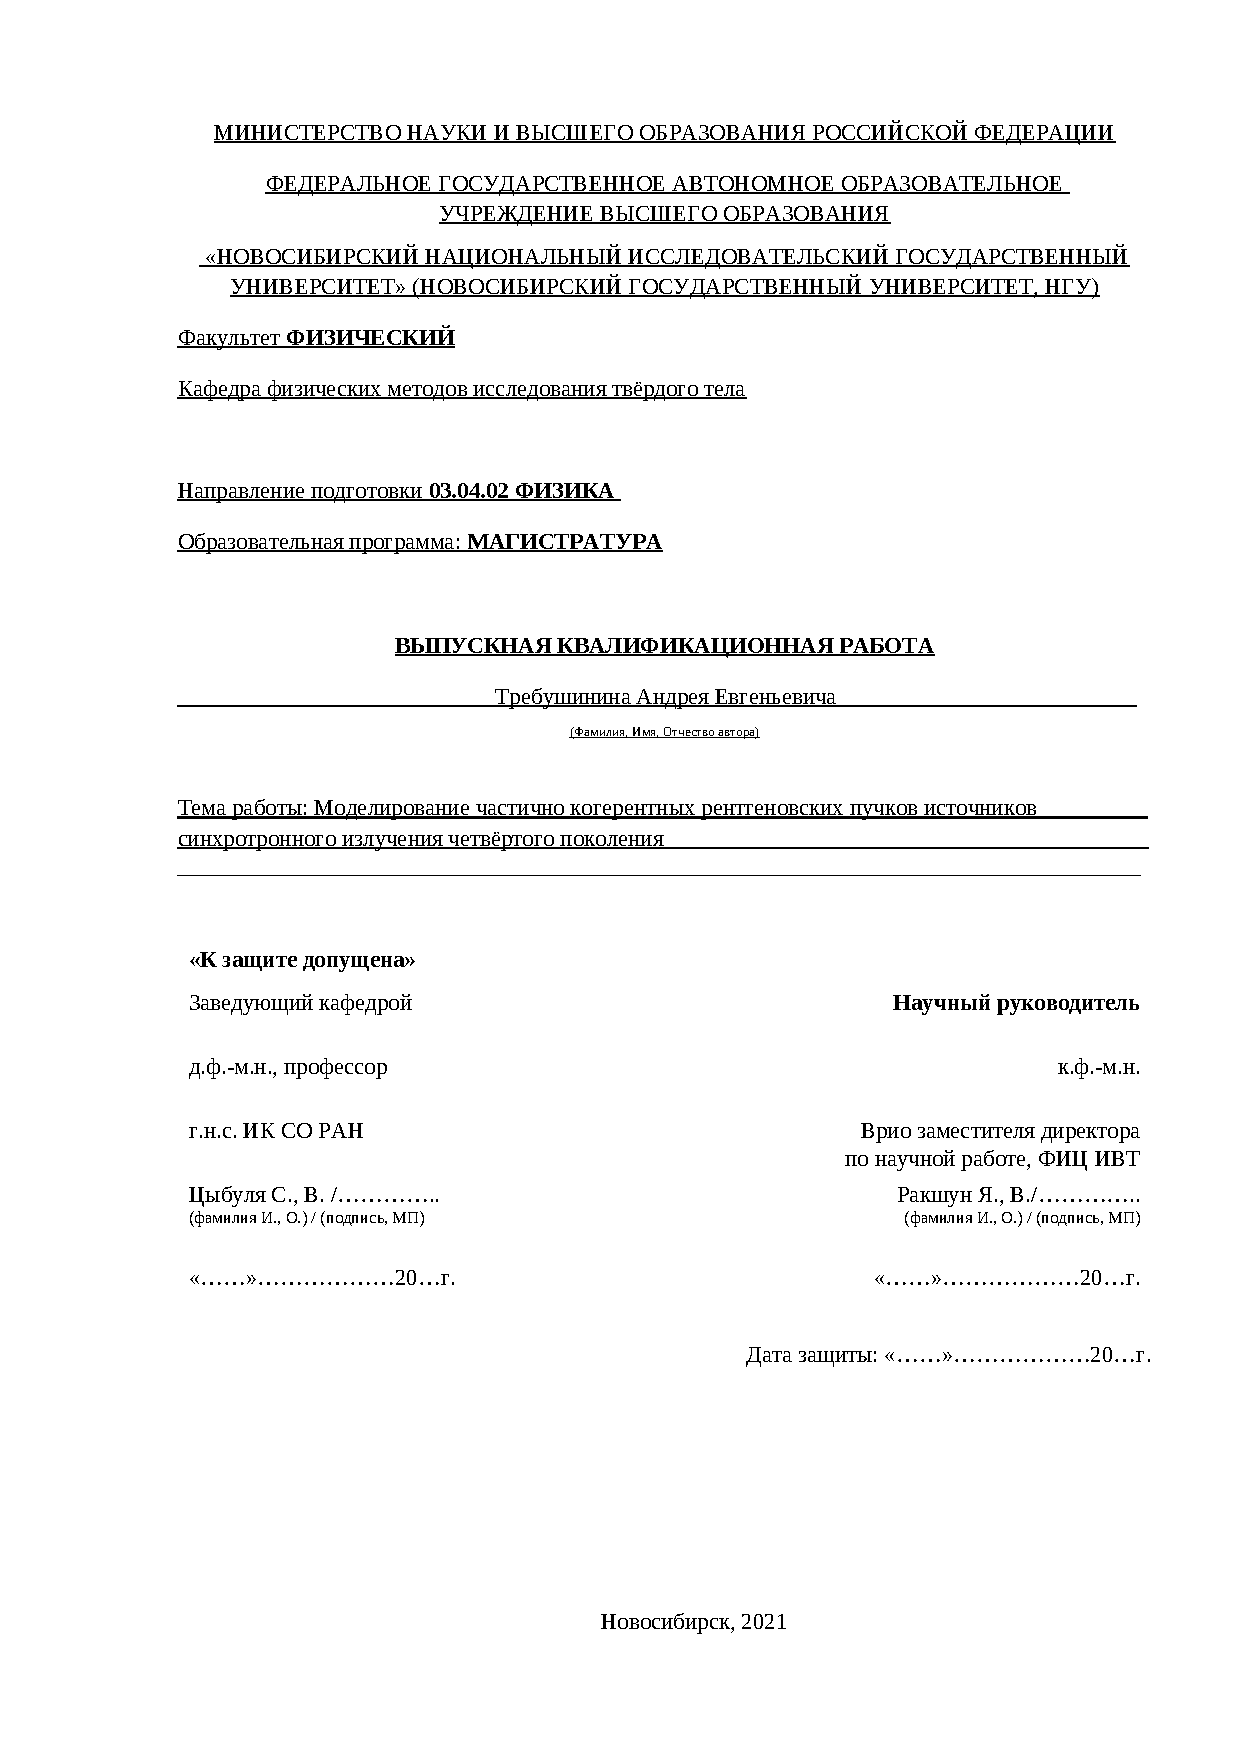
\includepdf{NSU/title}    % Титульный лист от НГУ
%% Ставим одинарный междустрочный интервал
\singlespacing
% Ставим геометрию для титульной страницы.
\newgeometry{left=3cm,right=1.5cm,top=2cm,bottom=2cm}

% Просто информация. Нигде в странице не используется, но зато попадёт в pdf info.
\author{Семенов А.\:В.}
\title{Измерение сечения e+ e- -> KS KL pi0}
\date{2017 г.}

\begin{titlepage}

%%%%%%%%%%%%%%%%%%%%%%%%%%%%%%%%%%%%%%%%%%%%%%%%%%%%%%%%%%%%%%%%%%%%%%%%%%%%%%%%

\begin{center}
    {\fnt{10.5} МИНИСТЕРСТВО ОБРАЗОВАНИЯ И НАУКИ РОССИЙСКОЙ ФЕДЕРАЦИИ} \\
        \vspace{0.3\baselineskip}
    {\fnt{10.5} ФЕДЕРАЛЬНОЕ ГОСУДАРСТВЕННОЕ АВТОНОМНОЕ ОБРАЗОВАТЕЛЬНОЕ \\ 
		\vspace{-0.3\baselineskip}
		УЧРЕЖДЕНИЕ ВЫСШЕГО ОБРАЗОВАНИЯ} \\
        \vspace{0.3\baselineskip}
    {\fnt{10.5} <<НОВОСИБИРСКИЙ НАЦИОНАЛЬНЫЙ ИССЛЕДОВАТЕЛЬСКИЙ ГОСУДАРСТВЕННЫЙ \\
		\vspace{-0.3\baselineskip}
		УНИВЕРСИТЕТ>> (НОВОСИБИРСКИЙ ГОСУДАРСТВЕННЫЙ УНИВЕРСИТЕТ, НГУ)}
\end{center}

%%%%%%%%%%%%%%%%%%%%%%%%%%%%%%%%%%%%%%%%%%%%%%%%%%%%%%%%%%%%%%%%%%%%%%%%%%%%%%%%

\vspace{0.5\baselineskip}

\noindent
{\fnt{11}Факультет}
$\overset{\text{\fnt{11}\textbf{ФИЗИЧЕСКИЙ}}\phantom{\hspace{10.9cm}}}{\underline{\hspace{0.88\textwidth}}}$

\vspace{0.3\baselineskip}

\noindent
{\fnt{11}Кафедра}
$\overset{\text{\fnt{11}\textbf{ФИЗИКИ ЭЛЕМЕНТАРНЫХ ЧАСТИЦ}}\phantom{\hspace{4.8cm}}}{\underline{\hspace{0.895\textwidth}}}$

\vspace{1\baselineskip}

\noindent
{\fnt{11}Направление подготовки}
$\overset{\text{\fnt{11}\textbf{03.03.02 ФИЗИКА}}\phantom{\hspace{8cm}}}{\underline{\hspace{0.73\textwidth}}}$

\vspace{0.3\baselineskip}

\noindent
{\fnt{11}Образовательная программа}
$\overset{\text{\fnt{11}\textbf{БАКАЛАВРИАТ}}\phantom{\hspace{7.3cm}}}{\underline{\hspace{0.69\textwidth}}}$

%%%%%%%%%%%%%%%%%%%%%%%%%%%%%%%%%%%%%%%%%%%%%%%%%%%%%%%%%%%%%%%%%%%%%%%%%%%%%%%%

\vspace{\baselineskip}

\begin{center}\bfseries
    {\fnt{11} ВЫПУСКНАЯ КВАЛИФИКАЦИОННАЯ РАБОТА БАКАЛАВРА} \\
\end{center}

%%%%%%%%%%%%%%%%%%%%%%%%%%%%%%%%%%%%%%%%%%%%%%%%%%%%%%%%%%%%%%%%%%%%%%%%%%%%%%%%

\vspace{0.3\baselineskip}

\noindent
$\overset{\text{\fnt{11}Семенов Александр Владимирович}}
{\underset{\text{\fnt{9}(фамилия, имя, отчество автора)}}{\underline{\hspace{\textwidth}}}}$

%%%%%%%%%%%%%%%%%%%%%%%%%%%%%%%%%%%%%%%%%%%%%%%%%%%%%%%%%%%%%%%%%%%%%%%%%%%%%%%%

\vspace{\baselineskip}

\noindent
{\fnt{11}Тема работы}
$\overset{\text{\fnt{11}Измерение сечения процесса e+e- -> KS KL pi0 с детектором КМД-3}}{\underline{\hspace{0.855\textwidth}}}$

\noindent
$\overset{}{\underline{\hspace{\textwidth}}}$

\noindent
$\overset{}{\underline{\hspace{\textwidth}}}$

%%%%%%%%%%%%%%%%%%%%%%%%%%%%%%%%%%%%%%%%%%%%%%%%%%%%%%%%%%%%%%%%%%%%%%%%%%%%%%%%

\vspace{2\baselineskip}

\noindent
\begin{tabular}{@{}p{0.5\textwidth}@{}@{}R{0.5\textwidth}@{}}
\fnt{11}\textbf{<<К защите допущена>>} &  \\
\fnt{11}Заведующий кафедрой,           & \fnt{11}\textbf{Научный руководитель} \\
\fnt{11}канд. физ.-мат. наук, доцент   & \fnt{11}канд. физ.-мат. наук, \\
\fnt{11}зав. лаб ИЯФ СО РАН            & \fnt{11}н.с. ИЯФ СО РАН\\
$\overset{\text{\fnt{11}Эйдельман, С.\,И.}}{\underset{\text{\fnt{8}(фамилия, И.\,О.)}}{\underline{\hspace{0.225\textwidth}}}}
\overset{\text{\fnt{11}/}}{}
\overset{\text{\fnt{11}}}{\underset{\text{\fnt{8}(подпись)}}{\underline{\hspace{0.125\textwidth}}}}$ &
$\overset{\text{\fnt{11}Шебалин, В.\,Е.}}{\underset{\text{\fnt{8}(фамилия, И.\,О.)}}{\underline{\hspace{0.225\textwidth}}}}
\overset{\text{\fnt{11}/}}{}
\overset{\text{\fnt{11}}}{\underset{\text{\fnt{8}(подпись)}}{\underline{\hspace{0.125\textwidth}}}}$ \\
$\overset{\text{\fnt{11}<<}}{}
\overset{\text{\fnt{11}}}{\underline{\hspace{0.05\textwidth}}}
\overset{\text{\fnt{11}>>}}{}
\overset{\text{\fnt{11}}}{\underline{\hspace{0.215\textwidth}}}
\overset{\text{\fnt{11}2017 г.}}{}$ & 
$\overset{\text{\fnt{11}<<}}{}
\overset{\text{\fnt{11}}}{\underline{\hspace{0.05\textwidth}}}
\overset{\text{\fnt{11}>>}}{}
\overset{\text{\fnt{11}}}{\underline{\hspace{0.215\textwidth}}}
\overset{\text{\fnt{11}2017 г.}}{}$ \\
& \\
& \fnt{11}\textbf{Консультант} \\
& \fnt{11}канд. физ.-мат. наук, \\
& \fnt{11}с.н.с. ИЯФ СО РАН\\
&
$\overset{\text{\fnt{11}Кардапольцев, Л.\,В.}}{\underset{\text{\fnt{8}(фамилия, И.\,О.)}}{\underline{\hspace{0.225\textwidth}}}}
\overset{\text{\fnt{11}/}}{}
\overset{\text{\fnt{11}}}{\underset{\text{\fnt{8}(подпись)}}{\underline{\hspace{0.125\textwidth}}}}$ \\
&
$\overset{\text{\fnt{11}<<}}{}
\overset{\text{\fnt{11}}}{\underline{\hspace{0.05\textwidth}}}
\overset{\text{\fnt{11}>>}}{}
\overset{\text{\fnt{11}}}{\underline{\hspace{0.215\textwidth}}}
\overset{\text{\fnt{11}2017 г.}}{}$
\end{tabular}

%%%%%%%%%%%%%%%%%%%%%%%%%%%%%%%%%%%%%%%%%%%%%%%%%%%%%%%%%%%%%%%%%%%%%%%%%%%%%%%%

\vspace{1.5\baselineskip}

\begin{flushright}
\fnt{11}
$\overset{\text{\fnt{11}Дата защиты: <<}}{}
\overset{\text{\fnt{11}}}{\underline{\hspace{0.05\textwidth}}}
\overset{\text{\fnt{11}>>}}{}
\overset{\text{\fnt{11}}}{\underline{\hspace{0.215\textwidth}}}
\overset{\text{\fnt{11}2017 г.}}{}$
\end{flushright}

%%%%%%%%%%%%%%%%%%%%%%%%%%%%%%%%%%%%%%%%%%%%%%%%%%%%%%%%%%%%%%%%%%%%%%%%%%%%%%%%

\vfill

\begin{center}
    \fnt{11} Новосибирск, 2017
\end{center}

\end{titlepage}

% Возвращаем всё назад: полуторный интервал и геометрию.
\onehalfspacing
\restoregeometry         % Титульный лист от НГУ
%\chapter*{Аннотация }							% Заголовок
Представленная работа посвящена разработке алгоритма моделирования частично когерентного синхротронного излучения и его применения для расчёта нескольких рентгенооптических оптических схем. В работе рассматриваются теоретические основы процесса генерации и распространения частично когерентного синхротронного излучения, а также его статистические характеристики. По ходу изложения приводится описание двух известных методов моделирования частично когерентного излучения, первый из которых обсуждался в литературе, однако не был описан в программном коде и, соответственно, не применялся при расчёте рентгенооптических схем синхротронных источников излучения. С помощью этого метода в работе описан эффект влияния продольной когерентности излучения на его угловую расходимость. При этом второй метод широко используется, несмотря на то, что обладает рядом недостатков, обсуждаемых в работе. Оба метода дают физически достоверный результат для наблюдаемых интенсивностей синхротронного излучения, однако, только первый метод даёт физически правильные поля излучения. На основе проделанной работы по изучению статистических свойств синхротронного излучения, был создан алгоритм, называемый СЕРВАЛ, качественно отличающийся от уже известных подходов. Была проведена перекрёстная проверка СЕРВАЛа на совпадение генерируемого поля в источнике и дальней зоне, а также соответствующих функций поперечной когерентности. Применение СЕРВАЛ показано на примере трёх оптических схем: фокусировка при наличии конечной входной апертуры, классический двухщелевой эксперимент (интерферометр Юнга) и фокусировка рентгеновским зеркалом при наличии шероховатостей. В работе проанализированы границы применимости СЕРВАЛа и описано его быстродействие.
% Оглавление (ГОСТ Р 7.0.11-2011, 5.2)
\pagenumbering{gobble}
\tableofcontents
        % Оглавление
\chapter*{Введение}							% Заголовок
\addcontentsline{toc}{chapter}{Введение}	% Добавляем его в оглавление

\newcommand{\actuality}{}
\newcommand{\aim}{\textbf{Целью}}
\newcommand{\tasks}{задачи}
\newcommand{\defpositions}{\textbf{Основные положения, выносимые на~защиту:}}
\newcommand{\novelty}{\textbf{Научная новизна}}
\newcommand{\influence}{\textbf{Научная и практическая значимость}}
\newcommand{\reliability}{\textbf{Степень достоверности}}
\newcommand{\probation}{\textbf{Апробация работы.}}
\newcommand{\contribution}{\textbf{Личный вклад.}}
\newcommand{\publications}{\textbf{Публикации.}}

%{\actuality}
В настоящее время в Институте ядерной физики им. Г. И. Будкера СО РАН проводятся эксперименты на электрон-позитронном накопителе \text{ВЭПП-2000} \cite{VEPP} в диапозоне энергий от 320 МэВ до 2 ГэВ в системе центра масс. В местах встречи пучков установлены два детектора: криогенный магнитный детектор \text{КМД-3 \cite{CMD}} и сферический нейтральный детектор \text{СНД \cite{SND}.} Физическая программа экспериментов включает в себя измерение сечений электрон-позитронной аннигиляции в адроны на низких энергиях, а также измерение адронного вклада в вычисление аномального магнитного момента мюона {$(g-2)_\mu$}. Так как в данной области энергии расчеты в рамках пертурбативной квантовой хромодинамики невозможны, то основным источником изучения взаимодействия легких кварков являются данные, полученные в экспериментах. Набор экспериментальных данных с детектором \text{КМД-3} начат в декабре 2010 года. В апреле 2013 года эксперименты были остановлены в связи с модернизацией инжекционного комплекса \cite{status}. В конце 2016 года запущен новый инжекционный комплекс \text{ВЭПП-5 \cite{VEPP-5}} и возобновлен набор статистики детектором \text{КМД-3.}

 \aim\ данной работы является измерение сечения процесса {$e^+\:e^- \to K_{S}\:K_{L}\:\pi^0$}
 в области энергий от порога рождения \text{(1130 МэВ)} до \text{2 ГэВ.} В анализе процесса использовались данные, полученные в экспериментах 2011-2012 годов с детектором КМД-3. Интеграл светимости составил \text{$33.18$ пб$^{-1}$} в диапозоне энергий от \text{1.1 ГэВ} до \text{2 ГэВ. }
 %Процесс примечателен тем, что все три конечные частицы псевдоскалярные и имеют общую плоскость распада. Одно из главных физических свойства процесса - это нейтральность конечных частиц. (Ниже воткнуть.)
 %пересчитать точнее светимость для твоей области

В задачи данной работы входило:
\begin{enumerate}
  \item Выработать оптимальные критерии отбора событий для процесса {$e^+\:e^- \to K_{S}\:K_{L}\:\pi^0$}.
  \item Определить эффективность регистрации процесса с помощью Монте-Карло моделирования.
  \item Получить предварительное сечение процесса {$e^+\:e^- \to K_{S}\:K_{L}\:\pi^0$} в диапозоне энергий от порога рождения \text{(1130 МэВ)} до \text{2 ГэВ.}
\end{enumerate}

%\novelty\ данной работы заключается в исследовании малоизученного процесса  {e^+\:e^- \to $\itshape K_{S}\:K_{L}\:\pi^0$}, а так же измерение его вклада в поляризацию ваакума, используемое для вычисления аномального магнитного момента мюона {$(g-2)_\mu$}.

Сечение данного процесса до недавнего времени не было измерено, в настоящее время существуют пока что только предварительные результаты, представленные коллаборацией SND \cite{korneev}, и недавно опубликованная статья коллаборации BaBar \cite{BaBar}. %Результаты ранее сказанных коллабораций имеют различия в области энергий выше 1.8 ГэВ, таким образом, имеет место дополнительная задача --- подтвердить результаты одной из коллабораций.
%данной работы заключается в вычислении сечения процесса  {e^+\:e^- \to $\itshape K_{S}\:K_{L}\:\pi^0$} в настоящее время предварительно изммеренного коллаборациями BaBar и SND, а так же в измерении его вклада в поляризацию ваакума, используемое для вычисления аномального магнитного момента мюона {$(g-2)_\mu$}. %коряво

%Научная новизна заключается в том, что сечение данного процесса до сих пор не был измерен, в настоящее время существуют пока что только предварительные результаты, представленные коллаборациями Бабар и СНД.
%Сказать про физику здесь, изотопический спин, все частицы в одной плоскости, три псевдоскалярные частицы. % Характеристика работы по структуре во введении и в автореферате не отличается (ГОСТ Р 7.0.11, пункты 5.3.1 и 9.2.1), потому её загружаем из одного и того же внешнего файла, предварительно задав форму выделения некоторым параметрам

%% регистрируем счётчики в системе totcounter
\regtotcounter{totalcount@figure}
\regtotcounter{totalcount@table}       % Если поставить в преамбуле то ошибка в числе таблиц
\regtotcounter{TotPages}               % Если поставить в преамбуле то ошибка в числе страниц

%% на случай ошибок оставляю исходный кусок на месте, закомментированным
%Полный объём диссертации составляет  \ref*{TotPages}~страницу с~\totalfigures{}~рисунками и~\totaltables{}~таблицами. Список литературы содержит \total{citenum}~наименований.
%
Представленная работа посвящена разработке методов моделирования процесса генерации синхротронного излучения (СИ) от электронного пучка с конечным эмиттансом и прохождения этого излучения через оптическую систему. Развитие магнитных схем циклических ускорителей дало возможность снизить эмиттанс электронного пучка и приблизить источники СИ к дифракционному пределу для широкого диапазона длин волн, вплоть до жёсткого рентгена. Под дифракционным пределом мы понимаем, что эмиттанс электронного пучка $\epsilon_{x, y}$ много больше или, по крайней мерее, сравним с "эмиттансом" излучения -- $\lambda/4\pi$, то есть  $\epsilon_{x, y} \ll \lambda/4\pi$. Такое излучение характиризуется заметной степенью поперечной когерентностью. Случай с частичной когерентностью представляет наибольший интерес, так как именно он реализуется в большинстве практических случаях. В работе предложен оригинальный метод генерации частично когерентного синхротронного излучения и рассмотрены практические примеры распространения частично когерентного волнового фронта через оптическую систему источников СИ.

\rr{...}


    % Введение
%\chapter*{Литературный обзор} \label{lit_rev}
\addcontentsline{toc}{chapter}{Литературный обзор}	% Добавляем его в оглавление

В этой главе будут разобраны публикации и источники, на которых основывается представленная работа. В абзацах будут даны ссылки на работы, которые дают общее представление о источниках синхротронного излучения и их применение, и далее, более конкретно, ссылки на статьи касательно теории и методов моделирования частично когерентного СИ. \rr{...}

Общее введение в теорию источников синхротронного излечения и их применение может быть найдено в ряде книг:~\cite{willmott_introduction_2019},~\cite{alsnielsen_elements_2011},~\cite{onuki_undulators_2003}. В ~\cite{willmott_introduction_2019} и~\cite{alsnielsen_elements_2011} даются общие представления о источниках синхротронного излучения, и основных компонентах на рабочих станциях, разбирается теоретическая основа и практическое применение основных методик реализуемых с помощью синхротронного излучения (в частности, в рентгеновском диапазоне длин волн). В книге~\cite{onuki_undulators_2003} даётся введение в динамику электронного пучка в накопительных кольцах, устройство вставных устройств: поворотных магнитов, вигглеров и ондуляторов. Более глубокие 
разъяснения касательно ускорительной техники могут быть найдены в~\cite{wiedemann_particle_2015}.

Общих подход при моделировании распространения волнового фронта через оптическую линию рабочей станции основывается на подходах Фурье-оптики~\cite{goodman_introduction_2005}

\rr{Надо написать кем и когда было предсказано синхротронное излучение, когда было впервые наблюдено. Указать по датам развитие синхротронных источников излучения от 1 до 3 поколения. Показать новый milestone -- источники 4 поколения, появление дифракционно ограниченных источников. Показать развитие кодов для моделирования синхротронного излучения: от программ для ray-tracing до wavefront propagation от Чубаря. Указать, как происходит моделирование. Показать основыне методы моделирования частично когерентного излучения. Разложение по Гаусс-Шелл модам...написать, что не так с этим подходом (ссылка на статью Джанлуки). Рассказать, что излучение следует гауссовой статистике. }
%============================================================================================================================
           % Литературный обзор
\chapter{Теоретический базис} \label{chapt1}

Распространение функции взаимной когерентности~\ref{eq:g1} поля $E(r, \omega)$ через свободное пространство от некогерентных стационарных источников излучения описывается теоремой Ван Циттера - Цирнике \cite{van_cittert_wahrscheinliche_1934}, \cite{zernike_concept_1938}. 
\begin{align}
	g^{(1)} (r_1; r_2) = \cfrac{\big \langle \bar{E}(r_1) \bar{E}(r_2) \big \rangle}{\big \langle \bar{E}(r_1)\big \rangle \big \langle\bar{E}(r_2) \big \rangle}, 
	\label{eq:g1} 
\end{align}
где $\big \langle ... \big \rangle$ означает усреднение по статистическим реализациям поля. Теорема даёт связь между распределением интенсивности источника излучения $I(\xi, \eta)$ и функцией взаимной когерентности $g^{(1)} (r_1, r_2)$ через двумерное Фурье преобразование. 
\begin{align}
	g^{(1)} (x_1, y_1, x_2, y_2) = \cfrac{\kappa e^{-i\psi}}{(\bar{\lambda}z)^2} \iint \limits_{-\infty}^{+\infty} I(\xi, \eta) \exp{\big [(i \cfrac{2 \pi}{\bar{\lambda}z}) (\Delta x \xi + \Delta y \eta)\big]}d\xi d\eta, 
	\label{eq:van_cittert_zernike_theorem} 
\end{align}
где $\kappa = \bar{\lambda}^2 / \pi$, $\bar{\lambda}$ -- средняя длина волны квазимонохроматического источника излучения, $z$ -- расстояние до плоскости наблюдения от источника излучения, $\psi = \cfrac{\pi}{\bar{\lambda} z}\big[((x^2_2 + y^2_2) - (x^2_1 + y^2_1)) \big]$, а $\Delta x = x_2 - x_1$, $\Delta y = y_2 - y_1$

Теорема может быть видоизменена и сформулирована для частично когерентных источников излучения достаточно лишь заменить $\kappa$ на двойной интеграл \cite{goodman_statistical_2015}
\begin{align}
	\kappa(\bar{x}, \bar{y}) = \iint \limits_{-\infty}^{+\infty} \mu(\Delta \xi, \Delta \eta) \exp{\big [(i \cfrac{2 \pi}{\bar{\lambda}z}) ( \bar{x} \Delta \xi + \bar{y} \Delta \eta)\big]}d\Delta \xi d\Delta \eta, 
\end{align}
где $\bar{x} = \cfrac{x_1 + x_2}{2}, \bar{y} = \cfrac{y_1 + y_2}{2}$,  $\Delta \xi = \xi_2 - \xi_1$, $\Delta \eta = \eta_2 - \eta_1$. Таким образом, следую модифицированной теореме ван Циттер-Цирнике, область пятна когерентности на расстоянии $z$ будет определяться не только размером источника излучения, но и размером области когерентности на самом источнике. 

В качестве примера распространения когерентности от полностью некогерентного источника можно оценить область когерентности излучения лабораторной рентгеновской трубки. Область когерентности от полностью некогерентного источника излучения квадратной формы получается напрямую из теоремы ван Циттер-Цирнике
\begin{align}
	A_c = \cfrac{(\bar{\lambda} z)^2}{A_s}.
\end{align}
Подставляя $z = 1$ м и $\lambda \approx 0.7$ $\textup{\AA}$ со спроецированной на направление выхода излучения из рентгеновской трубки площадью фокального пятна меньше чем $A_s = 1$ $\textup{мм}^2$ \cite{cullity_elements_1956}. Таким образом линейный размер длины когерентности при отражении от исследуемого кристалла с учётом угла дифракции ($= 45^{\circ}$) будет порядка $0.1$ $\textup{мкм}$. Однако линейный размер пятна когерентности может быть увеличен до нескольких микрон при использовании трубки с вращающимся анодом, где характерный диаметр круглого источника достигает $50$ $\textup{мкм}$ \cite{cullity_elements_1956}.  

Для синхротронных источников излучения область когерентности на источнике определяется натуральным размером излучения одного электрона при пролёте через вставное устройство. Например, в случае ондуляторного источника натуральный размер излучения определяется геометрическим размером перетяжки излучения в центре ондулятора. В случае рассмотрения излучения целого электронного пучка необходимо сравнивать размер излучения в перетяжке с размером электронного пучка. Для точного описания излучения от всего электронного пучка электромагнитное излучение может быть представлено как сумма полей от каждого индивидуального электрона. Каждый $k$ электрон в пучке имеет свою координату -- $\vec{\eta}_k$, угол -- $\vec{\l}_k$, отсчитываемые от проектной траектории, а также продольную координату или, другими словами, время прибытия $t_k$ относительно некоторого времени $t_0$, вклад которого в $r\omega$-пространстве будет умножением поля на фазовый фактор $\exp{(i \omega t_k)}$. Указанные величины подчиняются некоторым распределениям плотности вероятности, для накопительных колец в модельных случаях это распределение Гаусса. В данном случае не рассматривается разброс электронов по энергии, а дальнейшие описание можно найти в \cite{geloni_effects_2018}. Объём фазового пространства, который составляют эти шесть переменных, и есть эмиттанс электронного пучка. Результирующее поле от $N_e$ электронов можно записать следующим образом:
\begin{align}
	\bar{E}_{b} (z, \vec{r}, \omega) = \sum\limits_{k=1}^{N_e} \bar{E}(\vec{\eta}_k, \vec{\l}_k, z, \vec{r}, \omega) \exp{(i \omega t_k)},
	\label{eq:E_bunch} 
\end{align}
Для электронов в накопительных кольцах случайные величины $\vec{\eta}_k$ и $\vec{\l}_k$ не зависят от времени прибытия $t_k$. Модуля поля $\bar{E} = |\bar{E}_k|\exp{i\phi_k}$ имеет независящей от $k$ одинаковое распределение со средним $\big \langle|\bar{E}_k|\big \rangle$ и конечным вторым моментом  $\big \langle|\bar{E}_k|^2\big \rangle$. \rr{Всё это здорово, но должно откуда-то следовать. По всей видимости, эти предположения следуют из наличия дробового шума в электронном пучке (затухание и квантовая раскачка бетатронных колебаний). Нужна объяснительная команда.}.

Результирующее поле $\bar{E}_{b}$ является суммой вкладов от каждого электрона в пучке и по своей структуре в правой части уравнения~\ref{eq:E_bunch} записан некоторый фазор. Следуя предпосылкам центральной предельной теоремы (ЦПТ), можно показать, что $\bar{E}_{b}$ комплексная Гауссова переменная. Другими словами, амплитуда поля в каждой точке $\vec{r}$ подчиняется гауссовому распределению. Однако, предпосылки ЦПТ выполняются для двух практически значимых предельных случаев: случай длинного $\omega\sigma_T \gg 1$ и короткого электронного пучка $\omega\sigma_T \gg 1$, где $\sigma_T$ -- длительность электронного пучка \rr{а что не так с $\omega\sigma_T \sim 1$?}. В случае длинного электронного пучка величина $\omega t_k$ равномерно распределена в пределах от $0$ до $2\pi$ и излучение продольно некогерентно, для короткого пучка фазовый множитель $\exp{(i \omega t_k)}$ может быть взят равным единице и излучения является продольно когерентным. 

\rr{тут необходимо вернуться к идее о размер излучения одного электронна и размере электронного пучка}
\rr{так же где-то упомянуть о продольной спайковой структуре}
\newpage
%============================================================================================================================






           % Глава 1

\chapter{Методы моделирования ондуляторного излучения от пучка с конечным эмиттансом} \label{chapt2}
При обсуждении методов моделирования будет рассматриваться только ондуляторное излучение. Отчасти это мотивировано относительной простотой рассмотрения ондуляторного излучения, по сравнению, например, с вигглерным \cite{geloni_brightness_2014}, с другой стороны, при рассмотрении излучения источников четвёртного поколения,  излучение из ондуляторов обладает высокой степенью поперечной когерентности, что и представляет интерес данной работы. Тем не менее, формула~\ref{eq:E_bunch} применима как для ондуляторного излучения, так и для вигглерного и излучения из поворотного магнита. Для расчёта конечного поля по формуле~\ref{eq:E_bunch}, необходимо сгенерировать $N_e$ полей от каждого электрона и сложить их. Таким образом получиться одна реализация поля, далее необходимо повторить операцию генерации поля для $N_b$ реализаций и усреднить модули квадратов полей по получившемуся статистическому ансамблю. Метод получается крайне медленным и, в случае продольно некогерентного источника, для решения задачи моделирования источника излучения подойдёт метод реализованный в коде SRW \cite{chubar_accurate_1998}, \cite{chubar_simulation_2006}. Этот метод основан на сложение интенсивностей полей от каждого электрона, где нет необходимости усреднять по статистическому ансамблю, что ускоряет процесс моделирования. Оба метода будут обсуждаться в настоящей Главе. 

Альтернативный подход в моделировании частично когерентного излучения основывается на декомпозиции функции взаимной когерентности синхротронного излучения на Гауссовы-Шелл моды (разложение по полиномам Эрмита) описываемый в работах \cite{singer_modelling_2011}, \cite{hua_application_2012}, \cite{khubbutdinov_coherence_2019}, \cite{noauthor_iucr_nodate}. Однако, как отмечают сами авторы в \cite{khubbutdinov_coherence_2019}, \cite{noauthor_iucr_nodate} и аналитически описывается в \cite{geloni_transverse_2008}, разложение по полиномам Эрмита не применимо в случае, когда источник имеет высокую степень когерентности. Так как область когерентности на источнике весьма высока и функции, которые описывают поведение ондуляторного излучения как в дальней зоне, так и на источнике, имеют не гауссову природу.

В текущей главе описывается новый алгоритм моделирования синхротронного излучения, для краткости называемый СЕРВАЛ. Алгоритм основывается на прямом моделировании стохастических процессов при генерации синхротронного излучения, вызванных дробовым шумом в электронном пучке, с последующим ограничением пространственных гармоник шума огибающими излучения. По своей природе алгоритм имеет оценочный характер, именно поэтому в главе приведён сравнительный анализ результатов СЕРВАЛа с методом сложения амплитуд, на примере некоторых оптических систем. СЕРВАЛ показал себя как мощный инструмент для оценки когерентных свойств синхротронного излучения, с точностью мало уступающей методу сложения амплитуд, а главное имеющий преимущество в быстродействии. 
\section{Расчёт ондуляторного излучения прямым моделированием методом Монте-Карло}
Формула~\ref{eq:E_bunch} используется напрямую при моделирования монохроматизированного ондуляторного излучения, как продольно когерентного так и некогерентного. Общий вид поля ондуляторного излучения от одного электрона с некоторыми углом $\vec{\eta}_k$ и координатой $\vec{\l}_k$ может быть записан как \cite{geloni_fourier_2007}: 
\begin{align}
	\bar{E}_{\bot}(z_0, \omega, \vec{\eta}_k, \vec{l}_k, \vec{\theta} \;) =
&	-\frac{\omega e A_{JJ} L_w}{2c^2z_0}\frac{K}{\gamma}\exp{\bigg[i \frac{\omega z_0}{2c} \bigg|\vec{\theta} - \vec{\l}/z_0\bigg|^2 \bigg]} \cr & \times \sinc \bigg[\bigg(k_w \frac{\Delta \omega}{\omega} + \frac{\omega |\vec{\theta} - (\vec{\l}/z_0) - \vec{\eta}|^2}{2c}\bigg)\cfrac{L_s}{2}\bigg],
	\label{eq:single_electron_far_field}
\end{align}
где $\vec{\theta} = \vec{r}/z_0$, $e$ -- заряд электрона, $\gamma$ -- Лоренц-фактор, $K$ -- параметр ондуляторности, $k_w = 2 \pi / \lambda_w$, где $\lambda_w$ -- период ондулятора, $\Delta \omega$ -- отстройка от резонансной частоты. $A_{JJ} = J_0(\zeta) - J_1(\zeta)$, $\zeta = K^2/(4 + 2K^2)$ и $J_n$ -- функция Бесселя первого рода $n$ порядка. Формула \ref{eq:single_electron_far_field} даёт распределение амплитуды поля в дальней зоне, определения дальней зоны для ондуляторного излучения обсуждается в~\cite{geloni_fourier_2007}. Чтобы получить точное выражение, это поле должно быть распространено назад в центр ондулятора с помощью пропагатора\footnote{В дальнейшем изложении вместо слова «распространение» будет использоваться слово «пропогация»} свободного пространства~\cite{voelz_computational_2011},~\cite{schmidt_numerical_2010}. Распределение поля в мнимом источнике излучения:
\begin{align}
	\bar{E}_{\bot}(0, \vec{\eta}, \vec{\l}, \vec{r}_{\bot}) =
	i \frac{e A_{JJ} \omega}{2 c^2}\frac{K}{\gamma} &\exp{\big[i \frac{\omega}{c} (\vec{r}_{\bot} - \vec{l})\big]}\cr & \times \bigg [\pi - 2\text{Si} \bigg( \cfrac{i \omega |\vec{r}_{\bot} - \vec{l}|^2}{L_w c}\bigg)\bigg], 
	\label{eq:single_electron_near_field_z=0}
\end{align}
после этого поле можно распространять на любую дистанцию вдоль оптической оси $z_0$, что показано в~\cite{geloni_fourier_2007}, снова применяя пропагатор свободного пространства:
\begin{align}
	\bar{E}_{\bot}(&z_0, \omega, \vec{\eta}_k, \vec{\l}_k, \vec{r}) =
		\frac{e A_{JJ} \omega}{2 c^2}\frac{K}{\gamma} \exp{\bigg[i \frac{\omega}{2 z_0 c} (|\vec{r}_{\bot} - \vec{l}|^2 - |\vec{r}_{\bot} - \vec{l} - z_0 \vec{\eta}|^2) \bigg]} \cr & \times	\bigg \{ \text{Ei} \bigg[ \cfrac{i \omega (\vec{r}_{\bot} - \vec{l} - z_0 \vec{\eta})^2}{2z_0c - L_w c}\bigg] - \text{Ei} \bigg[ \cfrac{i \omega (\vec{r}_{\bot} - \vec{l} - z_0 \vec{\eta})^2}{2z_0c + L_w c} \bigg] \bigg\}.
	\label{eq:single_electron_near_field}
\end{align}
Рассчитанное таким образом поле может быть использовано для любого значения $z_0$, кроме точки $z_0 = L_w/2$ и $r_{\bot} = 0$, см.~\cite{geloni_fourier_2007}. Обе формулы \ref{eq:single_electron_far_field} и \ref{eq:single_electron_near_field} имеют практическую ценность при моделировании, стоит заметить, при использовании выражения \ref{eq:single_electron_near_field} время на моделирование значительно увеличивается, так как необходимо дважды численно взять интеграл $\textup{Ei}(\cdot)$.
 
\subsection{Метод сложения амплитуд}
После расчёта суммарного поля c $N_e$ электронами по формуле~\ref{eq:E_bunch}, получившиеся монохроматическое поле по своей сути есть одна статистическая реализация. Физически это значит следующее, если экспериментатор измерит распределение интенсивности поля на детекторе от пролёта одного электронного пучка, используя монохроматор с разрешением, которое позволит разрешить одну продольную моду излучения, то на детекторе будет распределение эквивалентное по своим свойствам распределению, представленному на Рис.~\ref{fig:spikes2} двумерным распределением интенсивности. 
\begin{figure}[H]
	\centering 	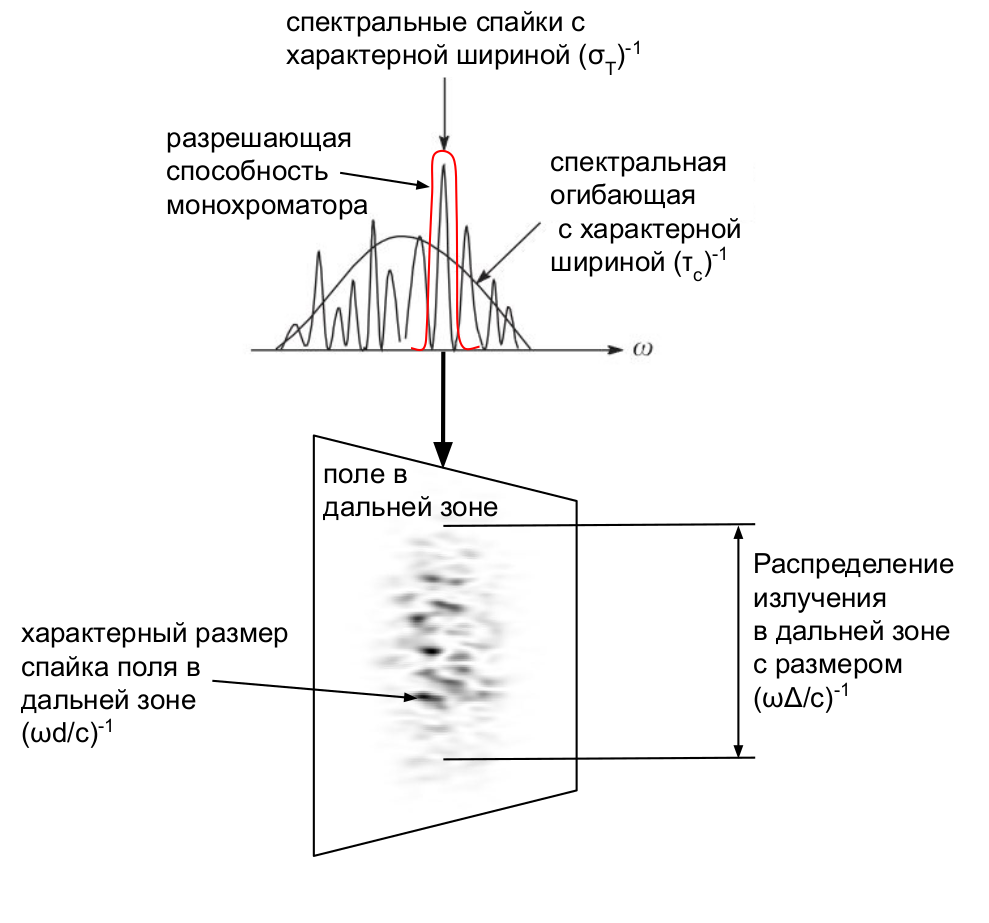
\includegraphics[width=0.7\linewidth]{spikes2.png}
	\caption{Спайковая структура излучения синхротронного излучения.}
	\label{fig:spikes2}
\end{figure}
После усреднения по $N_b$ реализациям (с идеальным монохроматором\footnote{другими словами, монохроматором разрешается одна поперечная мода}), наблюдаемая интенсивность даётся выражением: 
\begin{align}
	I_{\omega} = \bigg \langle \bigg|\sum\limits_{k=1}^{N_e} \bar{E}(\vec{\eta}_k, \vec{\l}_k, z, \vec{r}, \omega) \exp{(i \omega t_k)}\bigg|^2 \bigg \rangle,
	\label{eq:I_MC} 
\end{align}
\noindent результирующая интенсивность будет сходиться к некоторой огибающей. В грубом приближении огибающая является свёрткой распределения расходимости излучения и распределения расходимости электронного пучка. Общая схема метода сложения амплитуд изображена на Рис.~\ref{fig:MC_scheme}. 
\begin{figure}[H] 
	\centering 	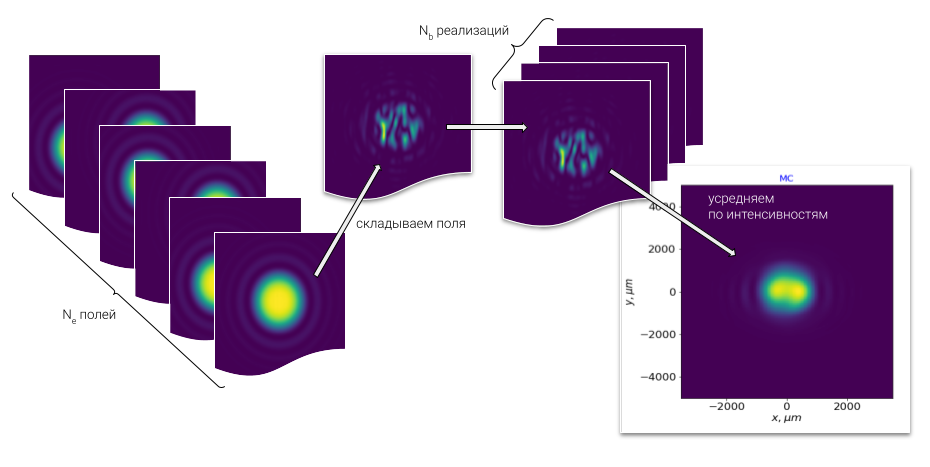
\includegraphics[width=0.99\linewidth]{MC_scheme.png}
	\caption{Схема работы метода сложения амплитуд}
	\label{fig:MC_scheme}
\end{figure}
Данный подход является наиболее прямым подходом в задаче моделирования частично когерентного излучения, однако время расчёта в таком случае может быть оценено как время затрачиваемое на расчёт одной одного поля $N_e$ раз по формуле~\ref{eq:single_electron_far_field} или~\ref{eq:single_electron_near_field}, в последней, как уже упоминалось, необходимо дважды численно взять интеграл $\textup{Ei}(\cdot)$ и потом усреднить по $N_b$ реализациям поля $\bar{E}_{b}$. Итого, если за $\tau_{calc}$ взять время расчёта одного поля формуле~\ref{eq:single_electron_far_field} или~\ref{eq:single_electron_near_field}, то расчёт одного результирующего поля $\bar{E}_{b}$ в сумме займёт $T_{calc} = \tau_{calc} \cdot N_e \cdot N_b$.

\subsection{Метод сложения интенсивностей}
В случае полностью некогерентного излучения время расчёта можно сократить за счёт фазового фактора $\exp{(i \omega t_k)}$, который эффективно приводит к тому, что излучение от отдельно электрона в электронном пучке коррелирует только с самим собой \cite{geloni_transverse_2008}. Если расписать выражение~\ref{eq:I_MC}. получим: 
\begin{align}
	I_{\omega} = \sum\limits_{k=1}^{N_e} \bar{E}(\vec{\eta}_k, \vec{\l}_k, z, \vec{r}, \omega)\bar{E}^{*}(\vec{\eta}_k, \vec{\l}_k, z, \vec{r}, \omega) + \cr
	\bigg \langle \sum\limits_{k=1}^{N_e} \sum\limits_{n=1}^{N_e} \bar{E}(\vec{\eta}_k, \vec{\l}_k, z, \vec{r}, \omega)\bar{E}^{*}(\vec{\eta}_n, \vec{\l}_n, z, \vec{r}, \omega) & \exp{\big[i \omega (t_k - t_n)\big]}\bigg \rangle,
	\label{eq:I_SRW_with_explicit_sum} 
\end{align}
где после усреднения, второе слагаемое будет равно нулю из-за упомянутого фазового фактора. Таким образом формула~\ref{eq:I_MC} упрощается до 
\begin{align}
 	I_{\omega} = \sum\limits_{k=1}^{N_e} \bigg|\bar{E}(\vec{\eta}_k, \vec{\l}_k, z, \vec{r}, \omega)\bigg|^2,
 	\label{eq:I_SRW} 
\end{align}
а время расчёта уменьшается до $T_{calc} = \tau_{calc} \cdot N_e$. Этот метод, для условности, будет носить название метод сложения интенсивностей. Общая схема метода представлена на Рис.~\ref{fig:SRW_scheme}.
\begin{figure}[H] 
	\centering 	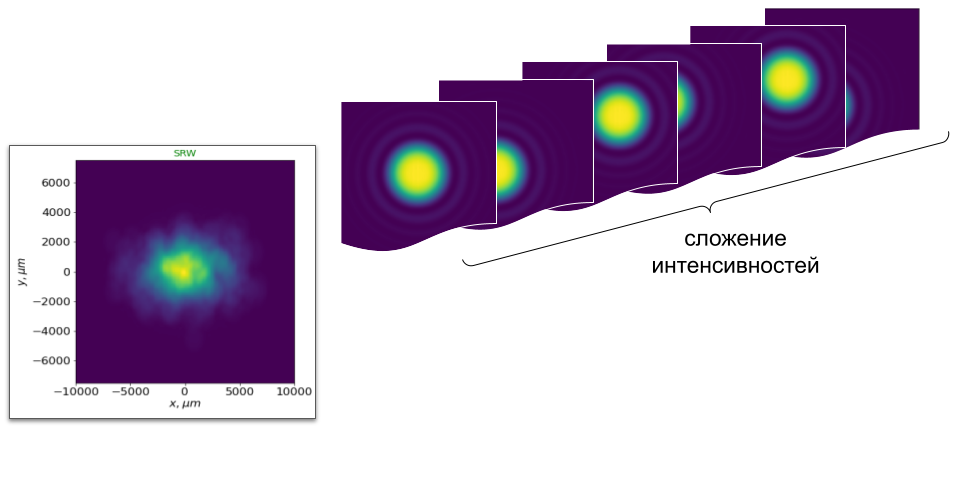
\includegraphics[width=0.99\linewidth]{SRW_scheme.png}
	\caption{Схема метода сложения интенсивностей}
	\label{fig:SRW_scheme}
\end{figure}
\noindent  Недостатком такого подхода можно считать потерю фазовой информации о излучении и, следовательно, невозможности расчёта функции взаимной когерентности первого порядка. Тем не менее, подход основанный на формуле~\ref{eq:I_SRW} даёт мощный метод расчёта наблюдаемых интенсивностей для частично когерентного излучения. Именно этот подход реализован в широко распространённом коде SRW.
  
\section{Учёт влияния размера электронного пучка на расходимость излучения при помощи прямых методов Монте-Карло}
С помощью описанные методов, а именно при помощи метода сложения амплитуд, можно получить поля, где будет видно влияние продольной когерентности\footnote{в смысле установленном в Главе~\ref{chapt1}} и размера электронного пучка на расходимость излучения.
\subsection{Влияние размера электронного пучка на расходимость излучения}
Первый эффект -- влияние размера электронного пучка на расходимость излучения и, следовательно на поперечный размер излучения в дальней зоне. Этот эффект обсуждается в работе~\cite{chubar_simulation_2006} разработчиком кода SRW применительно к когерентному синхротронному излучению (англ. coherent synchrotron radiation (CSR)). Под CSR подразумевает продольно когерентное излучение, реализуемое, когда электронный пучок много меньше излучаемой длины волны. На примере CSR можно наблюдать следующий эффект: если электронный пучок меньше или сравним с размером перетяжки излучения на источнике, наблюдается обычная расходимость излучения, определяемая свёрткой натуральной расходимости синхротронного излучения с расходимостью электронного пучка.
\begin{figure}[H]
	\centering 	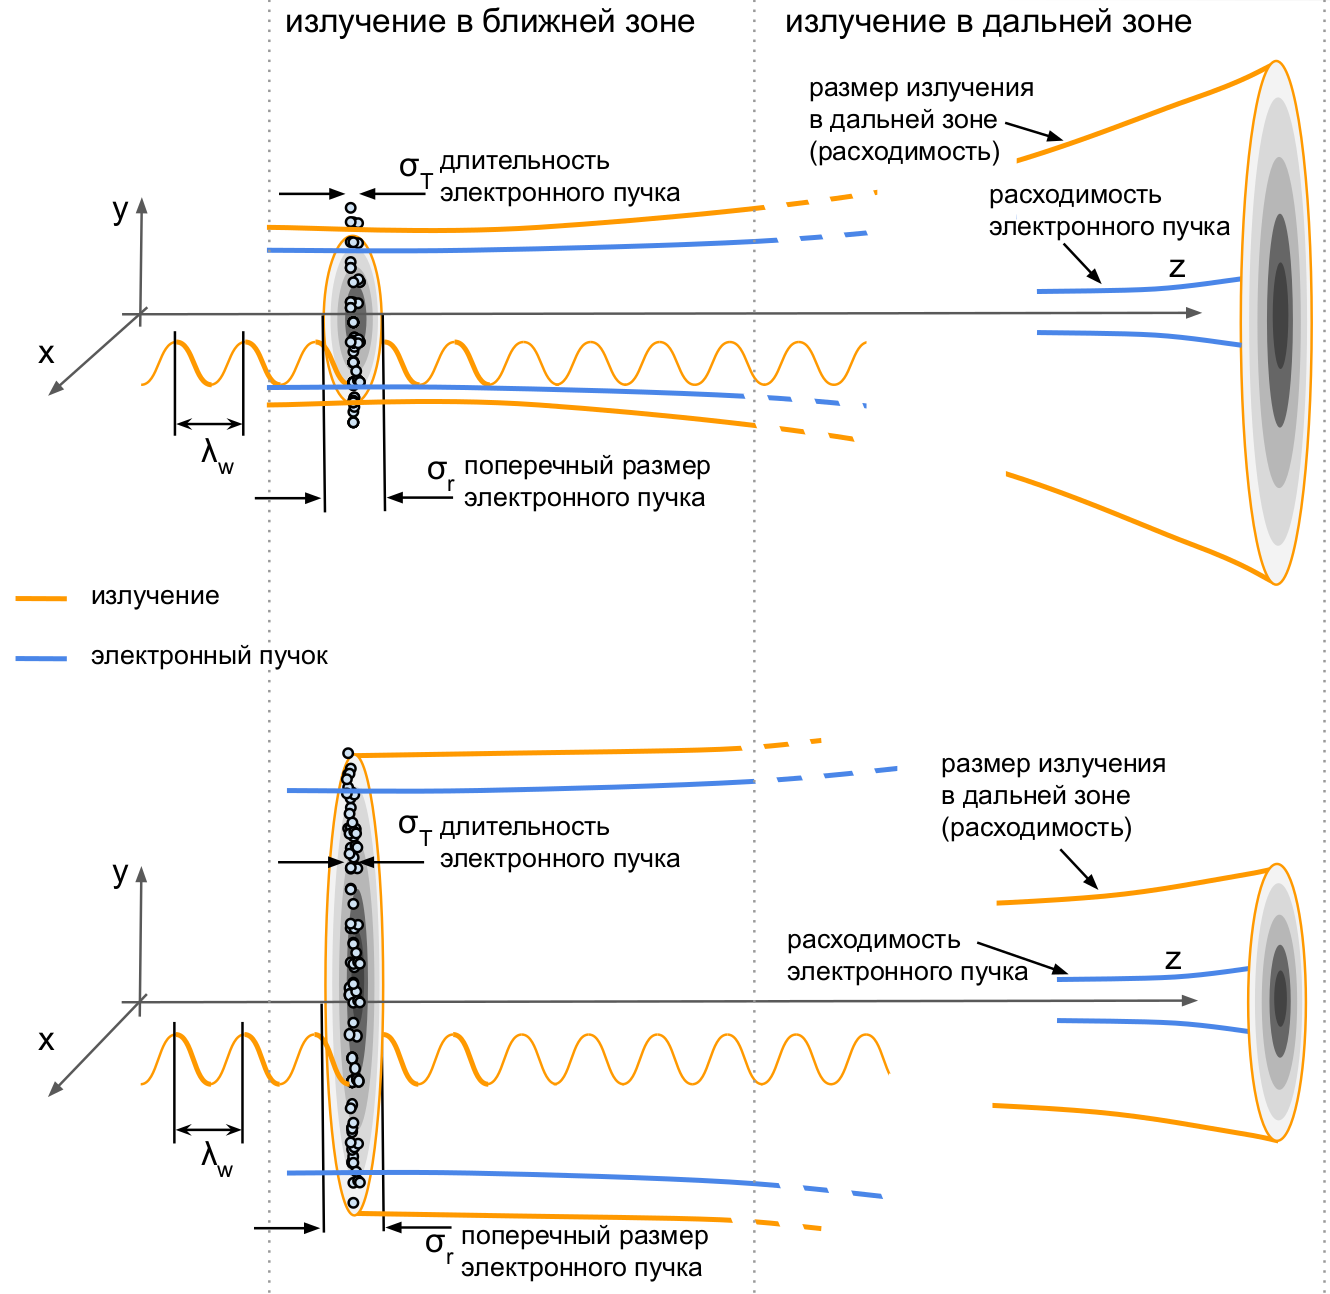
\includegraphics[width=0.99\linewidth]{diff_divergence_coh_scheme.png}
	\caption{Схема эффекта зависимости расходимости излучения от размера электронного пучка. Рисунок разделён на две части: ближняя зона, источник излучения -- слева и дальняя зона -- справа. Жёлтой линией схематично изображена характерный поперечный размер излучения, синей линей характерный поперечный размер электронного пучка, жёлтая волнистая линия символизирует длину волны излучения в сравнение с продольным размером электронного пучка. Важно отметить, что схематичный масштаб для обоих рисунков (верхнего и нижнего), -- тот же. Расходимости электронных пучков (сверху и снизу) одинаковы.}
	\label{fig:diff_divergence_coh_scheme}
\end{figure}
Однако, при увеличении размера электронного пучка, при той же расходимости, наблюдается эффект уменьшения расходимости излучения. Как отмечает автор в~\cite{chubar_simulation_2006}, этот эффект объясняется с точки зрения гауссовой оптики: при увеличении размера источника, угловой размер должен уменьшаться, формула~\ref{eq:photons_emittance}. На Рис~\ref{fig:diff_divergence_coh_scheme} изображена схема описывающая этот эффект.

При расчёт ондуляторного излучения методом сложения амплитуд этот эффект выглядит следующим образом, Рис.~\ref{fig:diff_coh_incoh_rad}.
\begin{figure}[H] 
	\centering 	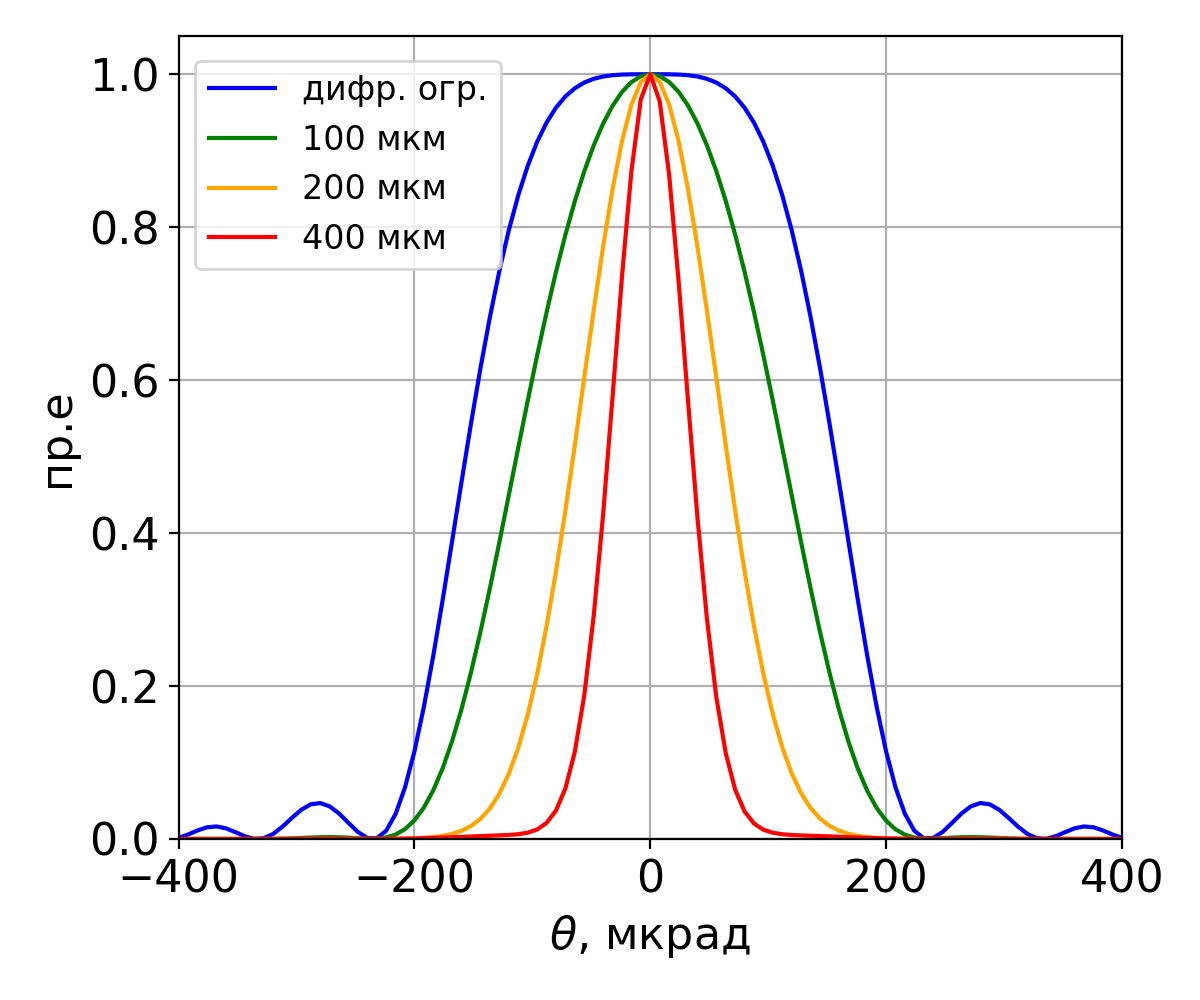
\includegraphics[width=0.5\linewidth]{diff_divergence_coh.png}
	\caption{Расходимость излучения от электронного пучка с размерами указанными в легенде. Расходимость электронного пучка много меньше натуральной расходимость синхротронного излучения}
	\label{fig:diff_coh_incoh_rad}
\end{figure}
Расчёт проводился для модельных параметров электронного пучка: расходимость была взята много меньшей чем натуральная расходимость ондуляторного излучения, размеры электронного указаны в легенде к Рис.~\ref{fig:diff_coh_incoh_rad}, резонансная энергия на $12,4$ эВ, ондулятор с $200$ периодами, длина периода $18$ мм. Синяя линия на Рис.~\ref{fig:diff_coh_incoh_rad} отвечает случаю электронного пучка с бесконечно малым эмиттансом.

\subsection{Различие расходимости излучения для случая продольно когерентного и некогерентного излучения}
В зависимости от длительности электронного пучка результирующее поле $\bar{E}_{b}$ будет вести себя по-разному. В случае короткого электронного пучка: $\omega \sigma_T \ll 1$, где $\sigma_T$ -- длительность электронного сгустка, излучение будет продольно когерентным, а в случай длинного электронного пучка, а именно  $\omega \sigma_T \gg 1$, соответствует продольно некогерентному излучению. 

\begin{figure}[H] 
	\centering 	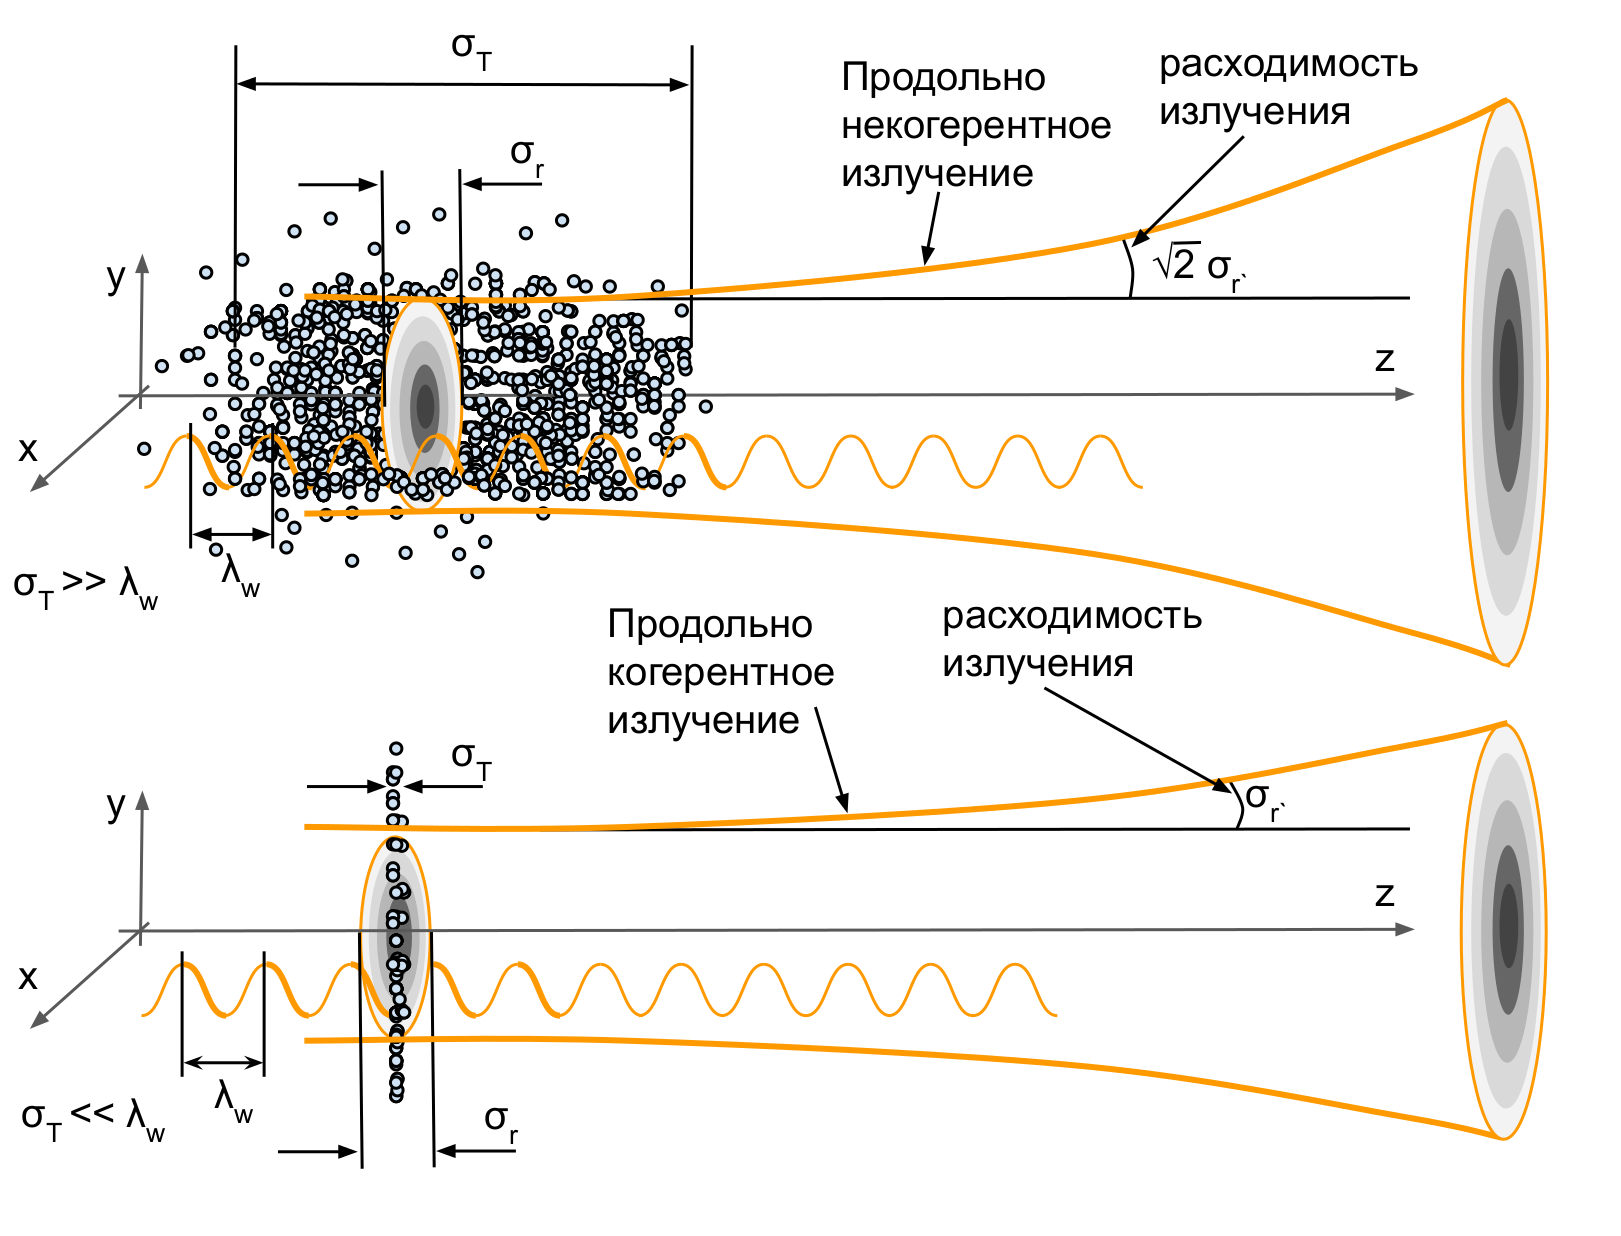
\includegraphics[width=0.99\linewidth]{coh_incoh_divergence.png}
	\caption{Схема эффекта зависимости расходимости излучения от продольной когерентности излучения. Жёлтой линией обозначен характерный поперечный размер излучения, жёлтой волнистой длина волны излучения с сравнение в продольным размером электронного пучка. На рисунке обозначено, что в случае продольно некогерентного излучения расходимость в $\sqrt{2}$ раз больше, чем в случае продольно когерентного излучения}
	\label{fig:coh_incoh_divergence}
\end{figure}
Расчёт проводился дли гипотетического случая электронного пучка с размерами пучка много меньшими натуральных размеров излучения в перетяжке\footnote{Чтобы для когерентного случая избежать эффекта, описанного в предыдущем разделе}, $\sigma_x' = 20$ мкрад, $\sigma_y' = 20$ мкрад на резонансное энергии $300$ эВ, ондулятором с $200$ периодами, длина периода $18$ мм. 

\begin{figure}[H] 
	\centering 	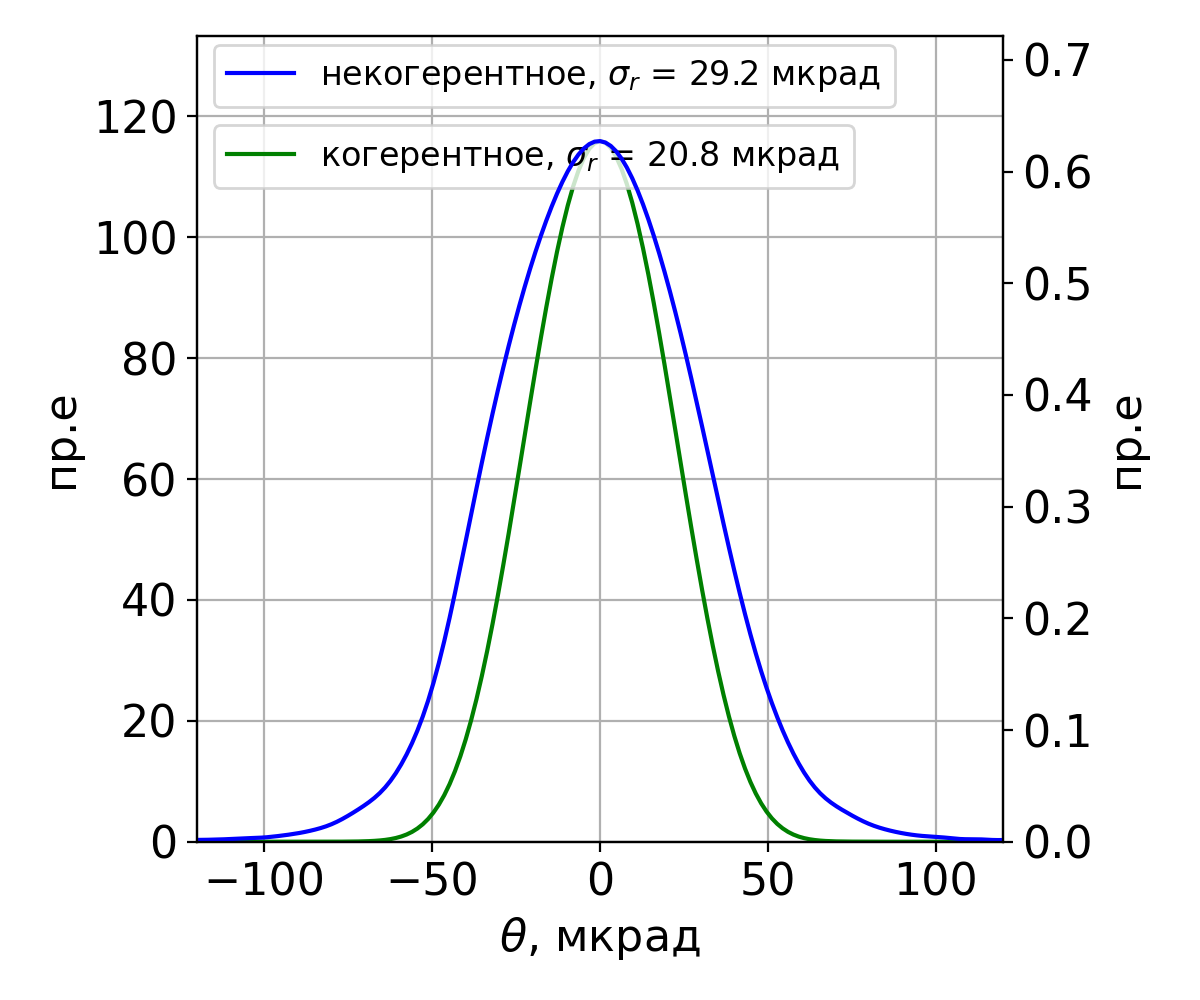
\includegraphics[width=0.5\linewidth]{diff_coh_incoh_rad.png}
	\caption{Расходимость излучения в случае продольно когерентного излучения (зелёная линия), и продольно некогерентного излучения (синяя линия).}
	\label{fig:diff_coh_incoh_rad}
\end{figure}
\noindent Этот эффект, по всей видимости, не обсуждался в литературе, однако заслуживает дальнейшего исследования.
\section{Метод ограничения пространственных гармоник огибающими: СЕРВАЛ}
Предлагаемый алгоритм основывается на моделировании стохастического характера ондуляторного синхротронного излучения комплексным гауссовым шумом с последующим его ограничением огибающими поля. Алгоритм описывает продольное некогерентное ондуляторное излучение. Для начала алгоритм будет представлен в общем виде, без уточнения чем определяются распределение огибающих, задающих размер и расходимость излучения и, в целом, безотносительно характера ондуляторного источника излучение. 
\subsection{Алгоритм создания поля}
Алгоритм, в целом стоит из трёх шагов: создание комплексного гауссового шума, его ограничение размерами излучения в перетяжке в $r$-пространстве и, в $k$-пространстве, расходимостью излучения\footnote{Излучение от всего электронного пучка.} в $k$-пространстве. Полное описание алгоритма приведено ниже: 
\begin{enumerate}
\item \label{noise} Создание комлексного гауссового шума $Z = X + iY$ в $r\omega$-пространстве, где величины $X$ и $Y$ подчиняются нормальному распределению.
\begin{figure}[H] 
	\centering 	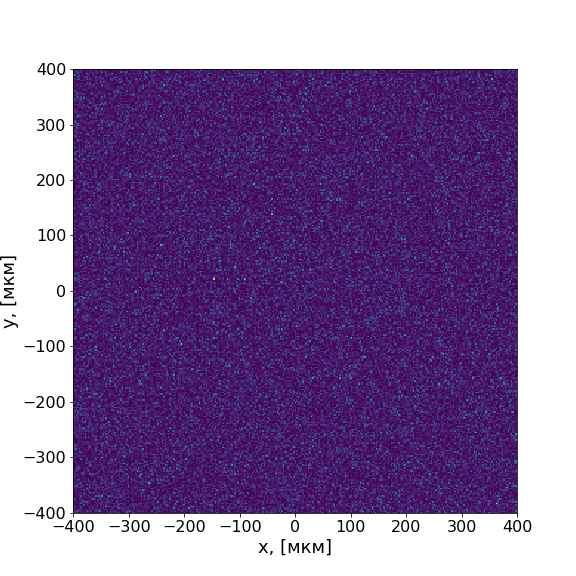
\includegraphics[width=0.45\linewidth]{1-X_noise.png}
	\caption{Интенсивность комплексного гауссового шума}
	\label{fig:1-noise}
\end{figure}
\item \label{beam_s} Ограничение шума эффективным размером электромагнитного излучения в источнике излучения в \textit{r$\omega$}-пространстве.
\begin{figure}[H]
	\centering
	\begin{minipage}{0.45\textwidth}
		\centering
		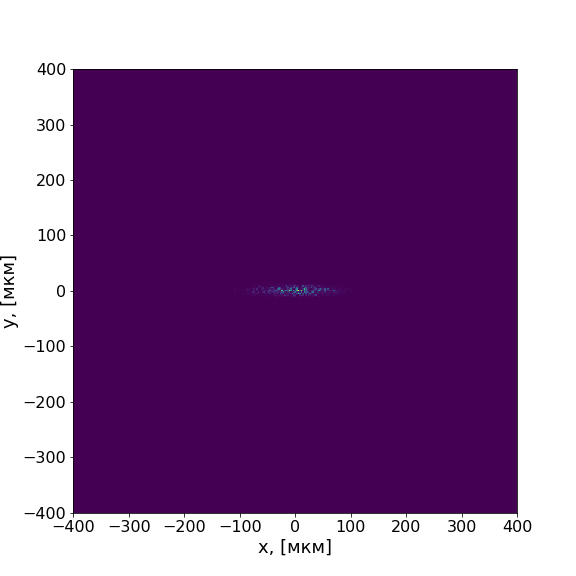
\includegraphics[width=1\linewidth]{2-X_e-beam-size.png}
		\caption{Размер излучения в перетяжке наложенное на комплексный гауссов шум}
		\label{fig:2-beam_size_k}
	\end{minipage}
	\begin{minipage}{0.45\textwidth}
		\centering
		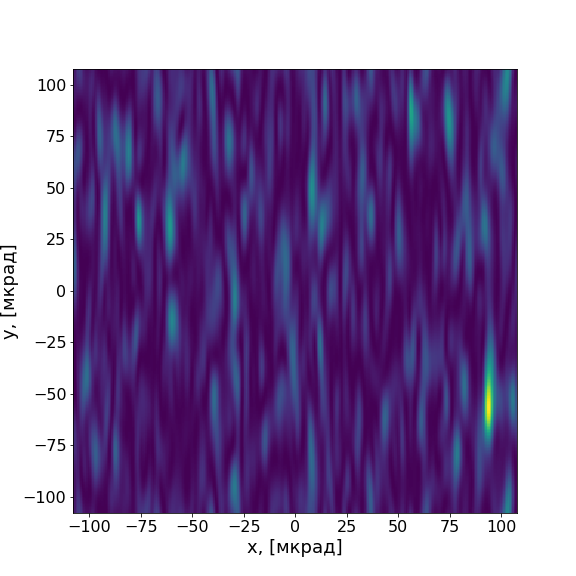
\includegraphics[width=1\linewidth]{2-X_e-beam-divergence.png}
		\caption{Получившиеся моды излучения в $k\omega$-пространстве}
		\label{fig:2-beam_size_s}
	\end{minipage}\hfill
\end{figure}
\item \label{beam_k} Ограничение пространственных мод эффективной расходимостью излучения в перетяжке в \textit{k$\omega$}-пространстве
\begin{figure}[H]
	\centering
	\begin{minipage}{0.45\textwidth}
		\centering
		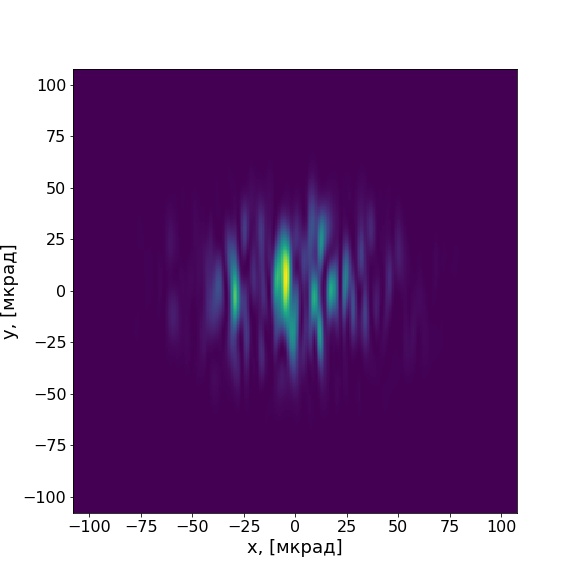
\includegraphics[width=1\linewidth]{3-X_radaition_divergence.png}
		\caption{Расходимость излучения в источнике}
		\label{fig:3-beam_s}
	\end{minipage}
	\begin{minipage}{0.45\textwidth}
		\centering
		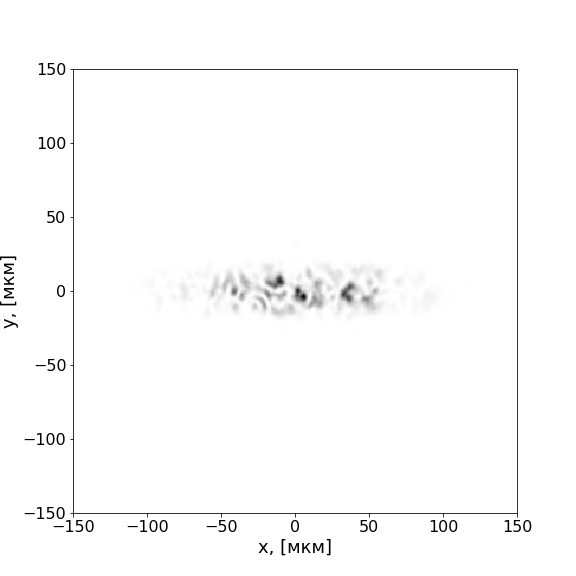
\includegraphics[width=1\linewidth]{3-X_radaition_size.png}
		\caption{Размер излучения в источнике}
		\label{fig:3-beam_k}
	\end{minipage}
\end{figure}
\item Получившиеся распространение поля есть распределение поля в источнике излучения (центр ондулятора).
\end{enumerate}
Быстродействие алгоритма можно оценить следующим образом: алгоритм генерирует $N_x \cdot N_y \cdot N_b$ случайный величин подчиняющихся распределению $Z$, где $N_b$ -- количество реализаций поля, одно Фурье преобразование поля (преобразование поля на Рис.~\ref{fig:2-beam_size_k} в поле на Рис.~\ref{fig:2-beam_size_s}) и две операции умножения на огибающие поля. Получившиеся поле, представленное на Рис.~\ref{fig:3-beam_k}, уже готово к пропагации, так как пропагатор через свободное пространство работает именно в $kf$-пространстве.
\subsection{Выбор подходящих огибающих}
До этого момента, в работе не обсуждался выбор подходящих огибающих для поля. Вопрос выбора таких огибающих сводится к нахождению распределения поля в центре ондулятора. Поле в центре ондулятора может быть получено обратной пропагацией излучения из дальней зоны обратно в центр ондулятора при помощи пропагатора излучения в свободном пространстве. Однако, нахождение аналитического решения уравнения Максвелла в дальней зоне от целого электронного пучка -- не тривиальная задача.  Для оценки можно предположить, что распределение поля ондуляторного излучения от электронного пучка с конечным эмиттансам, в целом, может быть представлено как свёртка распределения поля ондуляторного излучения от одного электрона с распределением фазового пространства электронного пучка~\cite{geloni_transverse_2008},~\cite{chubar_simulation_2006}.

Для SERVAL можно предложить, как минимум, три вида огибающих для пространственного распределения источника в $r$-пространстве:
\begin{enumerate}[label=\Roman*.]
	\item \label{amplitude} ${A}_{b} (\vec{r}_{\bot}) = \big(\bar{E}_{\bot}(0, \vec{l}, \vec{\eta}, \vec{r}_{\bot}) \ast f_l(\vec{l})\big)(\vec{l})$ \\

	\item \label{intensity} ${A}_{b} (\vec{r}_{\bot}) = \sqrt{\big(\bar{E}^2_{\bot}(0,  \vec{l}, \vec{\eta}, \vec{r}_{\bot}) \ast f_l^2(\vec{l})\big)(\vec{l})}$ \\

	\item \label{e-beam} ${A}_{b} (\vec{r}_{\bot}) = f_l(\vec{l})$,
\end{enumerate}
и три вида огибающих для распределения расходимости источника -- $k$-пространство:
\begin{enumerate}[label=\Roman*.]
	\item \label{amplitude} $\hat{{A}}_{b} (\vec{\theta}_{\bot}) = \big(\hat{\bar{E}}_{\bot}(0,  \vec{l}, \vec{\eta}, \vec{\theta}_{\bot}) \ast \hat{f}_{\eta}(\vec{\eta})\big)(\vec{\eta})$\\
	
	\item \label{intensity} $\hat{{A}}_{b} (\vec{\theta}_{\bot}) = \sqrt{\big(\hat{\bar{E}^2}_{\bot}(0,  \vec{l}, \vec{\eta}, \vec{\theta}_{\bot}) \ast \hat{f_{\eta}^2}(\vec{\eta})\big)(\vec{\eta})}$\\
	
	\item \label{e-beam} $\hat{{A}}_{b} (\vec{\theta}_{\bot}) = \hat{f}_{\eta}(\vec{\eta})$,
\end{enumerate}
где ${A}_{b} (\vec{r})$ и $\hat{{A}}_{b} (\vec{\theta})$ огибающие в $r$- и $k$-пространствах соответствующие шагам~\ref{beam_s} и~\ref{beam_k} в алгоритме,  $f(\vec{l}, \vec{\eta}) = f_l(\vec{l}) f_{\eta}(\vec{\eta})$ фазовое распределение электронного пучка, и поле $\bar{E}_{\bot}(z=0, \vec{\l}, \vec{\eta}, \vec{r}_{\bot})$, $\hat{\bar{E}}_{\bot}(z=0 , \vec{\l}, \vec{\eta}, \vec{\theta}_{\bot})$ -- распределение поля взятого в центре ондулятора по формулам \ref{eq:single_electron_far_field}(или более точно \ref{eq:single_electron_near_field}) и \ref{eq:single_electron_near_field_z=0}.

Для выбора подходящих амплитуд было проведено моделирование с различными огибающими в сравнение с эталонным в этой работе методом сложения амплитуд. Для начала необходимо проверить распределение интенсивности поля на источнике. Для метода сложения амплитуд поле было рассчитано в дальней зоне и отпропагировано назад в центр ондулятора. Результаты сравнения приведены на Рис.~\ref{fig:SERVAL_envelopes_comparison_far_zone} и представлены на Рис.~\ref{fig:SERVAL_envelopes_comparison_source}, Рис.~\ref{fig:SERVAL_corr_comparison}, Рис.~\ref{fig:SERVAL_envelopes_comparison_far_zone}. В работе использовались следующий параметры: ондулятора~\ref{tab:undulator_parameters}
\begin{table}[H]
	\caption{Параметры ондулятора}
	\label{tab:undulator_parameters}	
	\begin{tabular}{l|c|r}	
		$E_{ph},  [\textup{эВ}]/\lambda, [\textup{\AA}$]& $\lambda_w, [\textup{мм}]$ & $L, [\textup{м}]$\\ 
		\hline	%0.65-1.35
		2167/5.72    &  18      & 3.6   
	\end{tabular}
\end{table}
\noindent Расчёты будут проводиться для параметров электронного пучка ЦКП «СКИФ» для одного из прямых промежутков вставных устройств, которые представлены в Таблице~\ref{tab:SKIF parameters}
\begin{table}[H]
	\caption{Параметры электронного пучка}
	\label{tab:SKIF parameters}	
	\begin{tabular}{l|c|c|c|r}
		$E, \textup{[GeV]}$ & $\sigma_x, \textup{[мкм]}$ & $\sigma_y, \textup{[мкм]}$ & $\sigma_{x'}, \textup{[мкрад]}$ & $\sigma_{y'}, \textup{[мкрад]}$ \\ 
		\hline
		3          &38                          & 4.7                        & 25                          & 20 
	\end{tabular}
\end{table} 
\begin{figure}[H] 
	\centering 	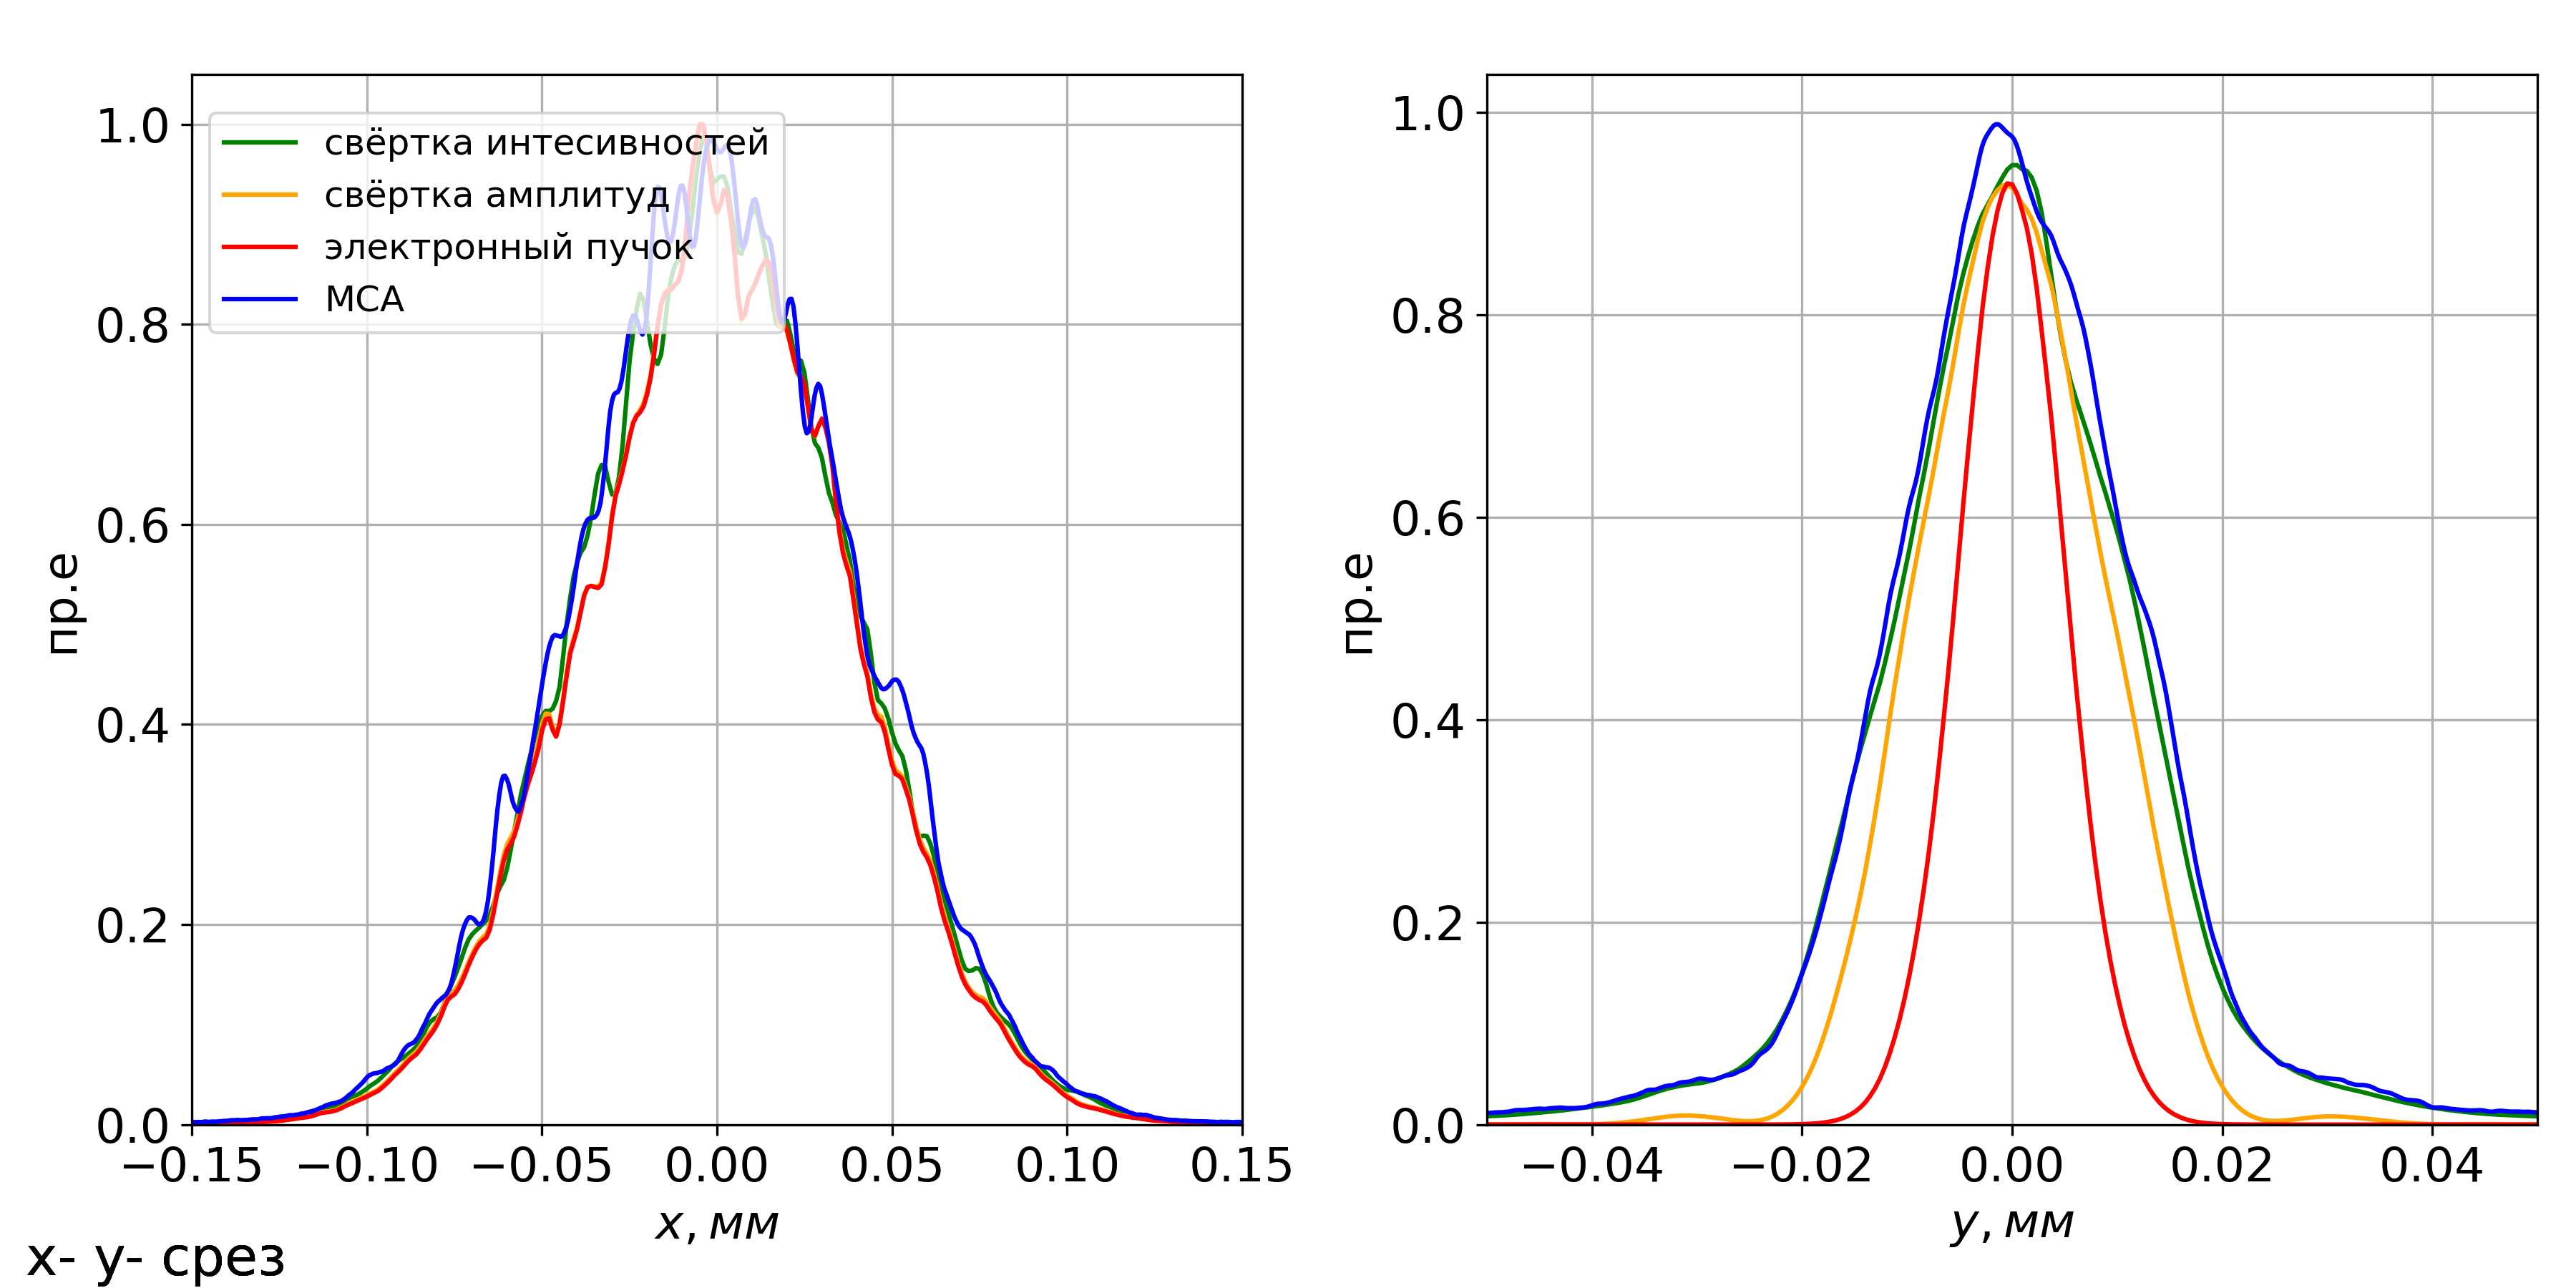
\includegraphics[width=0.99\linewidth]{SERVAL_envelopes_comparison_source.png}
	\caption{Распределение поля в источнике излучения}
	\label{fig:SERVAL_envelopes_comparison_source}
\end{figure}
Видно, что оптимальные результаты достигаются при использовании свёртки~\ref{intensity}. Однако, если размер электронного пучка много больше или даже сравним с натуральным размером излучения в перетяжке, то можно использовать любые из представленных огибающих для $r$-пространства. Необходимо так же сравнить корреляционные функции получившихся полей~\ref{fig:diff_coh_incoh_rad}, используя формулу~\ref{eq:g1}.
\begin{figure}[H] 
	\centering 	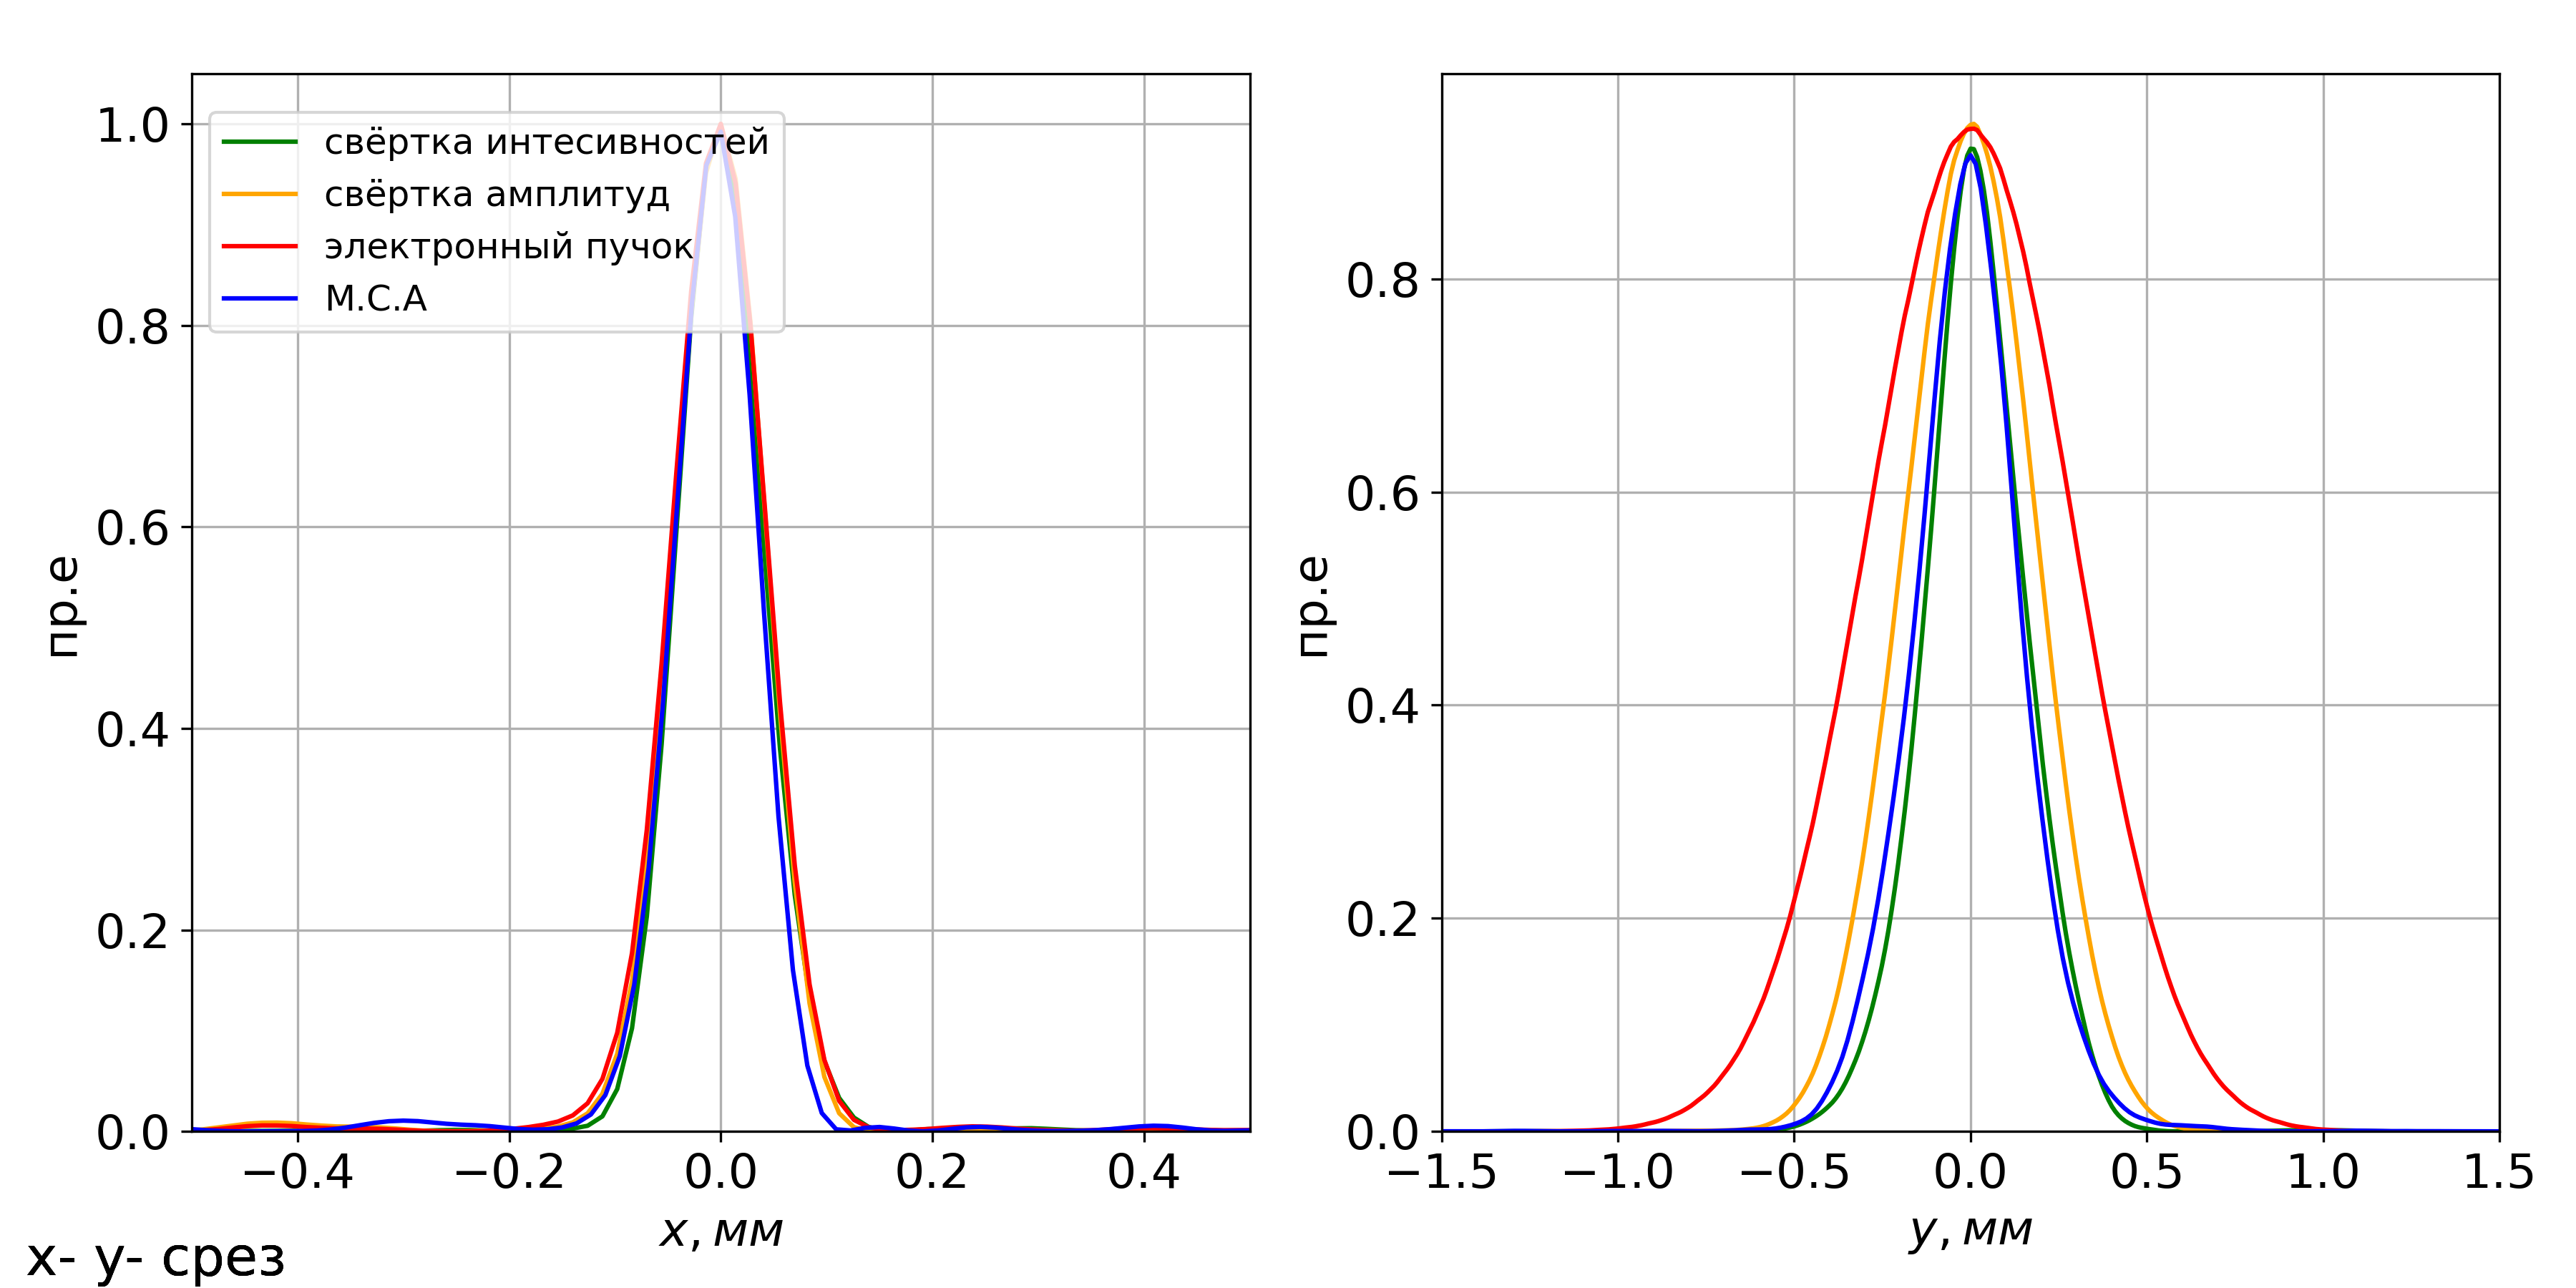
\includegraphics[width=0.99\linewidth]{SERVAL_corr_comparison.png}
	\caption{Функция взаимной когерентности на расстоянии $25$ м от источника}
	\label{fig:SERVAL_corr_comparison}
\end{figure}
\noindent Для распределения расходимости следует так же использовать использовать свёртку интенсивностей.
\begin{figure}[H] 
	\centering 	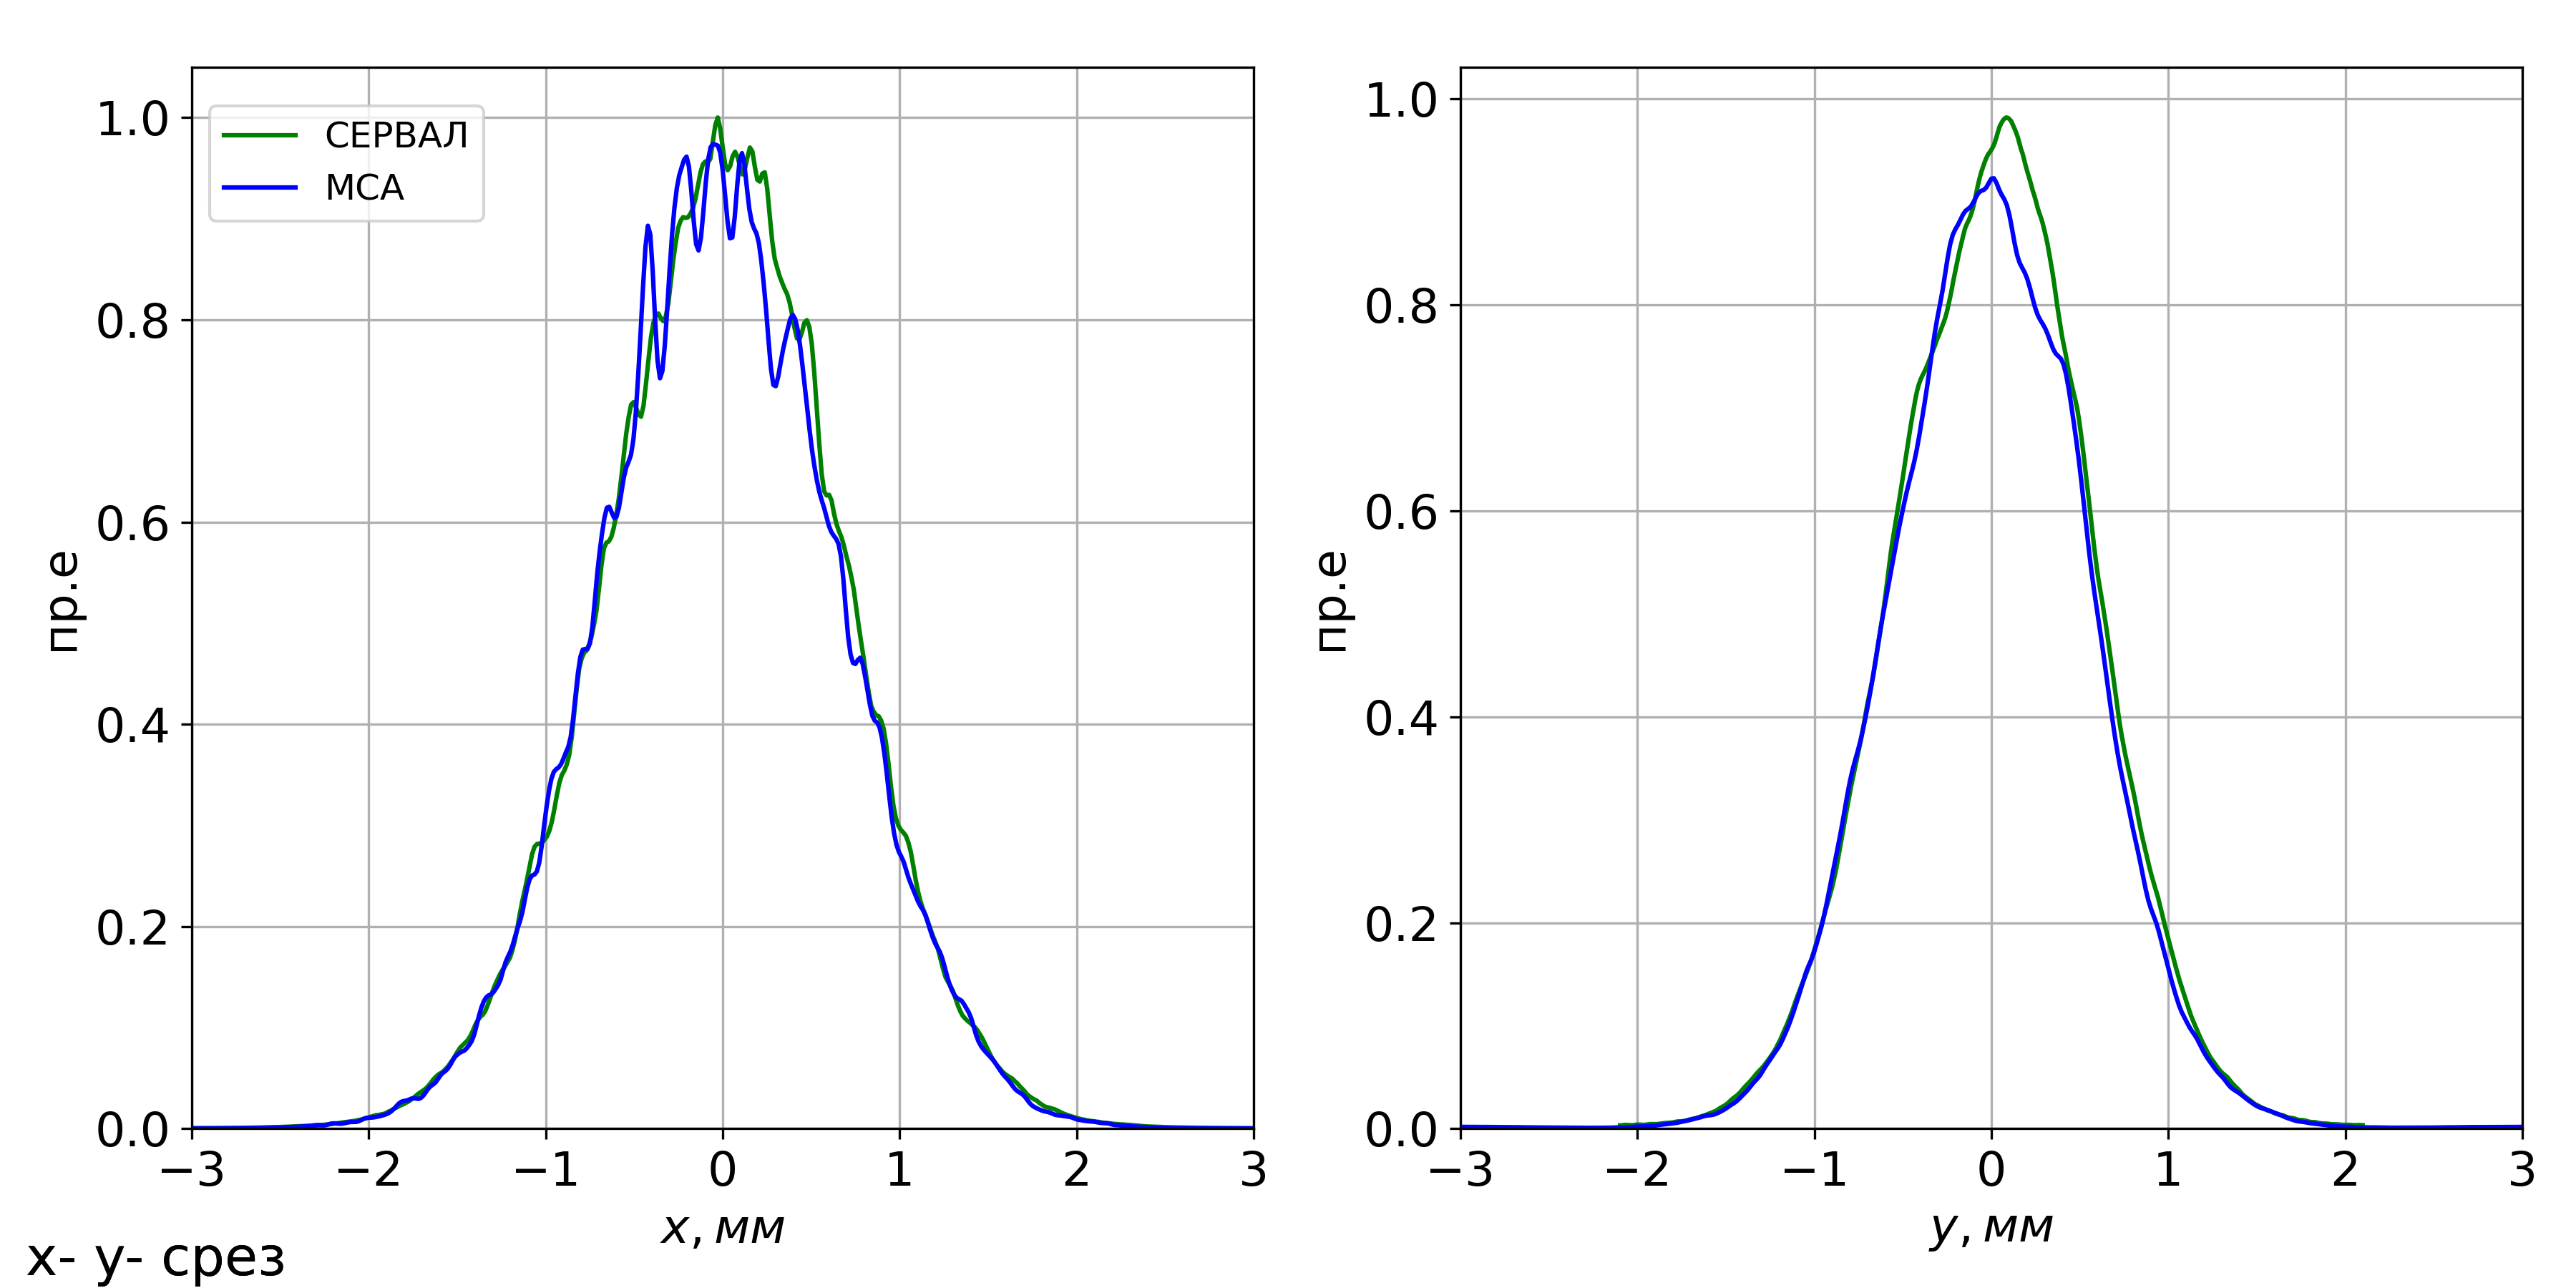
\includegraphics[width=0.99\linewidth]{SERVAL_envelopes_comparison_far_zone.png}
	\caption{Размеры излучения в дальней зоне (расходимость) на расстоянии $25$ м}
	\label{fig:SERVAL_envelopes_comparison_far_zone}
\end{figure}
В большинстве случаев можно выбирать свёртку интенсивностей по~\ref{intensity}. Однако, стоит отметить, что SERVAL -- это оценочный метод и в случае дифракционного ограниченного источника необходимо перед проведением расчётов сделать подобный анализ подходящих огибающих, Приложение~\ref{AppendixA}.

\chapter{Применение СЕРВАЛа} \label{chapt3}
СЕРВАЛ является эффективным алгоритмом для моделирования частично когерентного синхротронного излучения, в случаях когда есть заметная степень когерентности источника излучения. Уже было показано совпадение распределений интенсивности в дальней зоне и на источнике излучения, а так же совпадение корреляционных функций с методом сложения амплитуд, который может считаться методом, дающий результат «из первых принципов» во всех ситуациях\footnote{необходимо помнить, что число $N_e$ должно быть достаточно велико для получения достоверного результата}. Этот сравнительный анализ свойств источника излучения даёт все предпосылки, что весьма ресурсозатратный по времени метод сложения амплитуд может быть заменён СЕРВАЛом без потери точности и физичности результатов. В этой главе мы приведём ещё один сравнительный анализ СЕРВАЛа и метода сложения амплитуд на примере фокусирующей системы с конечной апертурой, а так же два практических применения СЕРВАЛа на примере простого эксперимента Юнга и нетривиальной задачи отражения частично когерентного излучения от рентгеновского зеркала с шероховатостями. 
Однако, отдельно необходимо отметить, когда источник дифракционно ограничен, целесообразно применять метод сложения амплитуд или метод сложения интенсивностей, которые очень быстро дадут сходимость. В этом случае для СЕРВАЛа потребуется тщательный анализ подходящих огибающих и, строго говоря, метод \textit{не моделируют} фундаментальную моду ондуляторного излучения -- случай излучения электронного пучка с бесконечно малым эмиттансом\footnote{случай, когда эмиттанс излучения много больше эмиттанса электронного пучка}. Для источников с низкой степенью когерентности имеет смысл рассмотреть метод трассировки лучей, в этом случае все три волновых метода будут иметь весьма низкую сходимость и придётся моделировать большое число статистических реализаций для получения сходимости. В любом случае, в каждом из рассмотренных случаев прежде чем проводить оптический расчёт, необходимо изучить свойства источника излучения, например при помощи программы SPECTRA~\cite{tanaka_spectra_2001}, оценить ожидаемую степень когерентности и только исходя из свойств источника применять один из описанных методов моделирования. Именно такой подход даст оптимальный результат в смысле затраченного времени и физичности полученных результатов. 

\section{Фокусирующая система с конечной апертурой}\label{section:focusing_system_with_aperture}
Рассмотрим оптическую систему состоящую из источника излучения -- ондулятора, апертуры и фокусирующего элемента. Для SERVAL были выбраны огибающие~\ref{intensity}. Этот расчёт будет сопровождаться сравнением результатов метода СЕРВАЛ с результатами метода сложения амплитуд (МСА).

\begin{figure}[H] 
	\centering 	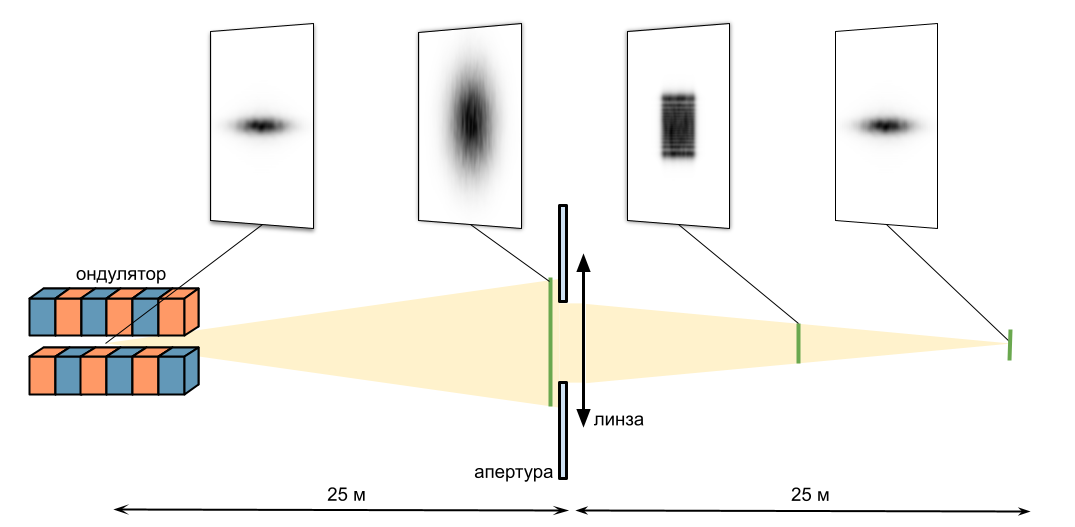
\includegraphics[width=0.99\linewidth]{beamline.png}
	\caption{Схема оптики}
	\label{fig:beamline}
\end{figure}
Распределение поля в дальней зоне на 25 м от ондулятора представлено на Рис.~\ref{fig:focusing_system_far_zone}.
\begin{figure}[H] 
	\centering 	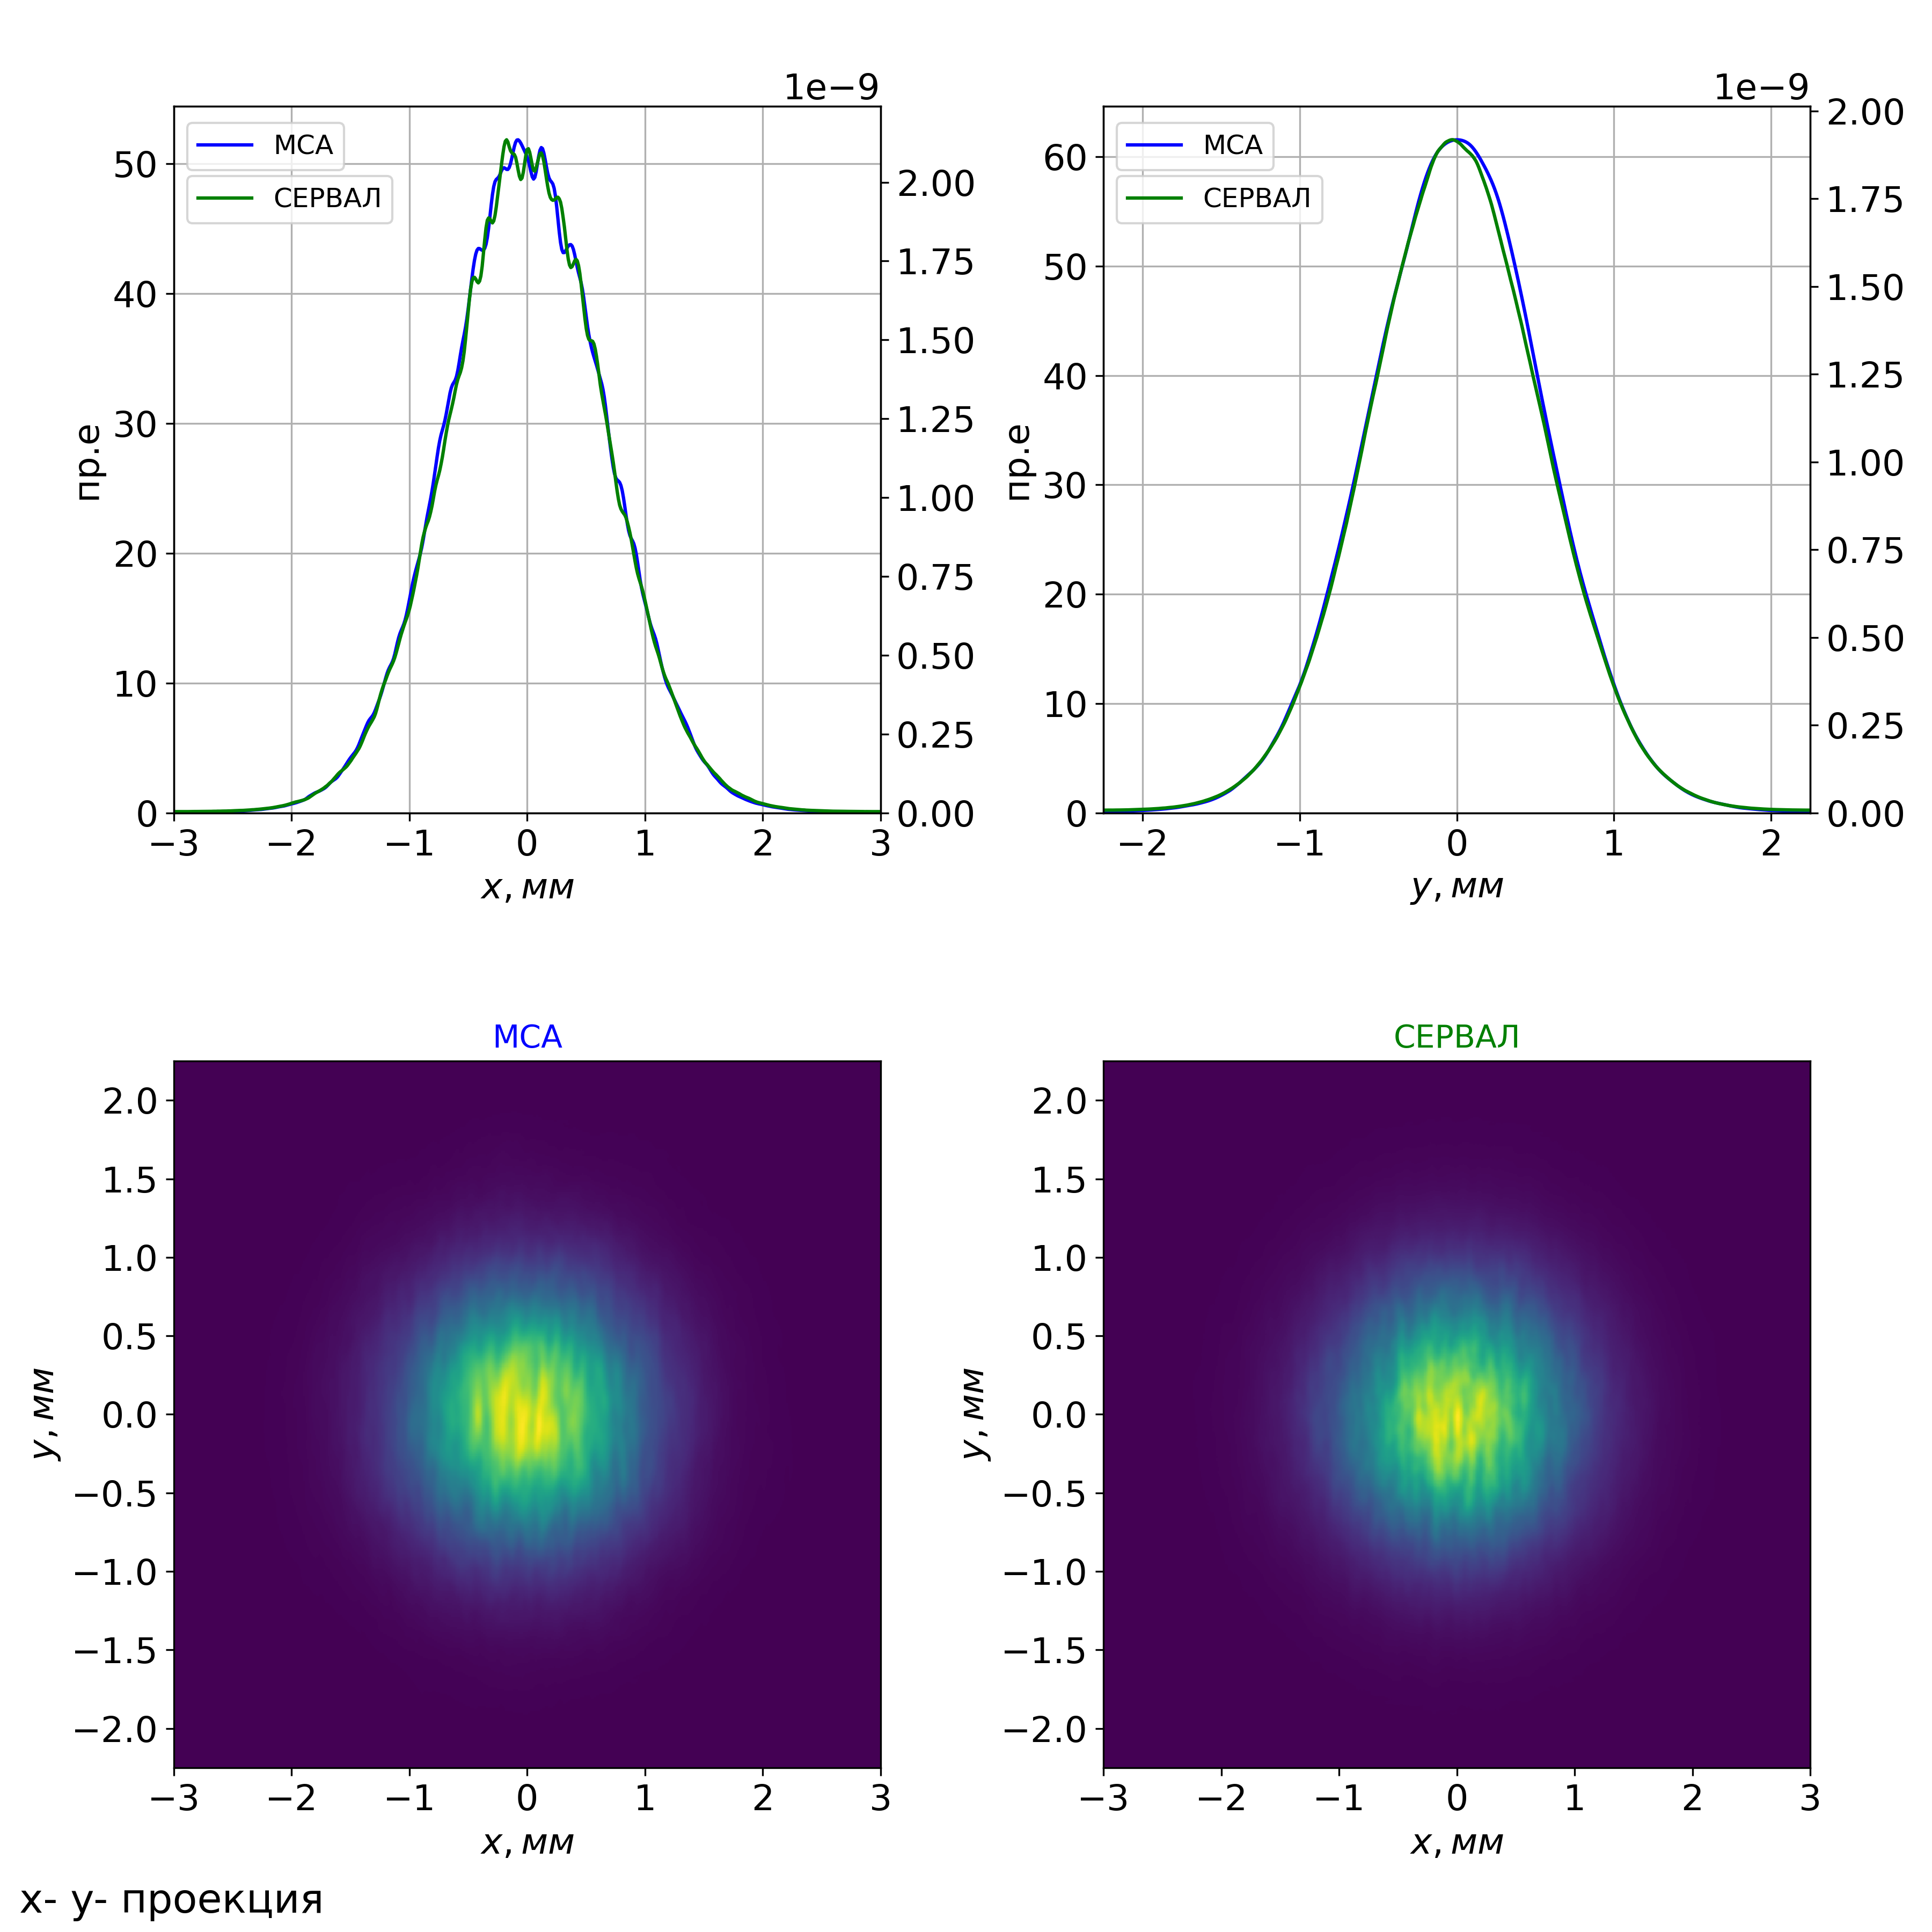
\includegraphics[width=0.99\linewidth]{1-far_zone_25_m3.80E-05_um_4.68E-06_um_2.50E-05_urad_2.00E-05_urad_example_beamline.png}
	\caption{Распределение интенсивности излучения в дальней зоне. \rr{$MCA_x, СЕРВАЛ_x = 1500$ мкм, $MCA_x, СЕРВАЛ_x = 1270$ мкм}}
	\label{fig:focusing_system_far_zone}
\end{figure}
Для усреднения было выбрано 300 реализаций, что даёт достаточную сходимость. Однако в структуре излучения всё ещё видна характерная модовая структура. Видно что количество мод в вертикальном направление меньше чем в горизонтальном, а их типичный размер говорит о длине поперечной когерентности в соответствующих направлениях. Размер пятна когерентности определяется через размер функции взаимной когерентности, представленной на Рис.~\ref{fig:focusing_system_corr}.
\begin{figure}[H] 
	\centering 	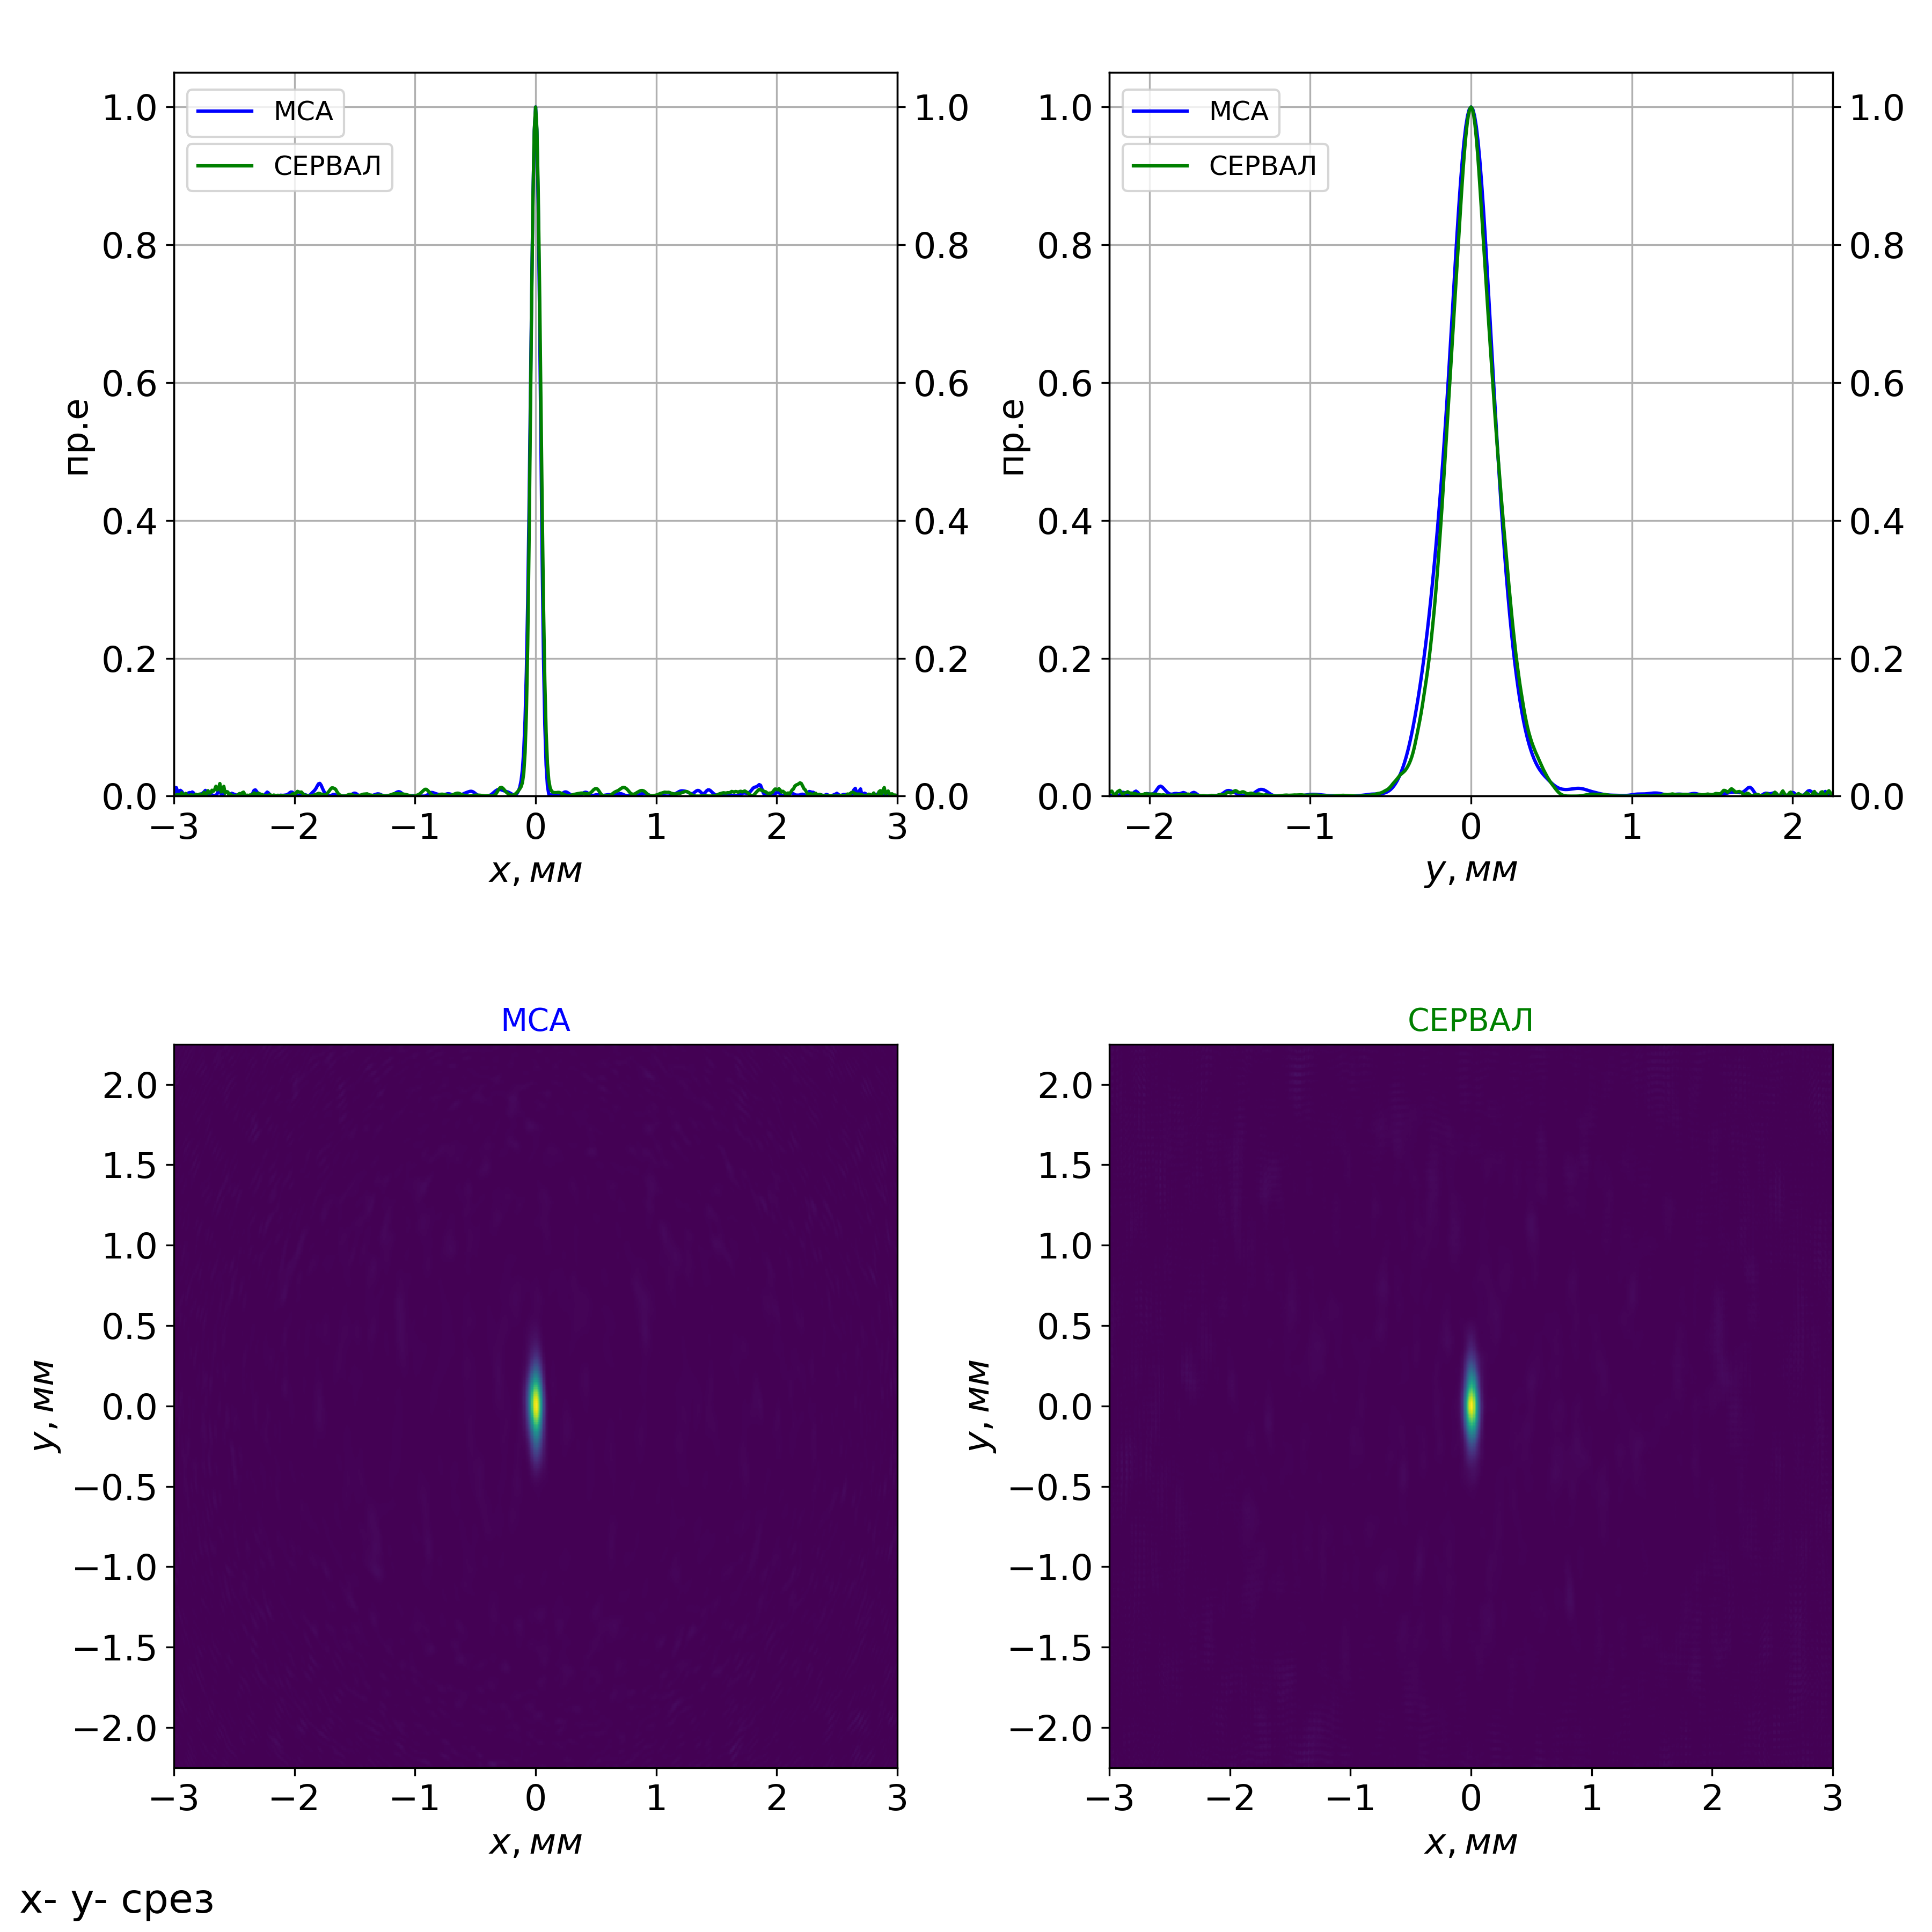
\includegraphics[width=0.99\linewidth]{corr3.80E-05_um_4.68E-06_um_2.50E-05_urad_2.00E-05_urad_example_beamline.png}
	\caption{Корреляционная функция, построенная по формуле~\ref{eq:g1}. \rr{$MCA_x, СЕРВАЛ_x = 87$ мкм, $MCA_x, СЕРВАЛ_x = 320$ мкм}}
	\label{fig:focusing_system_corr}
\end{figure}
\noindent После апертуры и 10 метров распространения поля через пустое пространство результат приведён на Рис.~\ref{fig:focusing_system_far_zone}
\begin{figure}[H] 
	\centering 	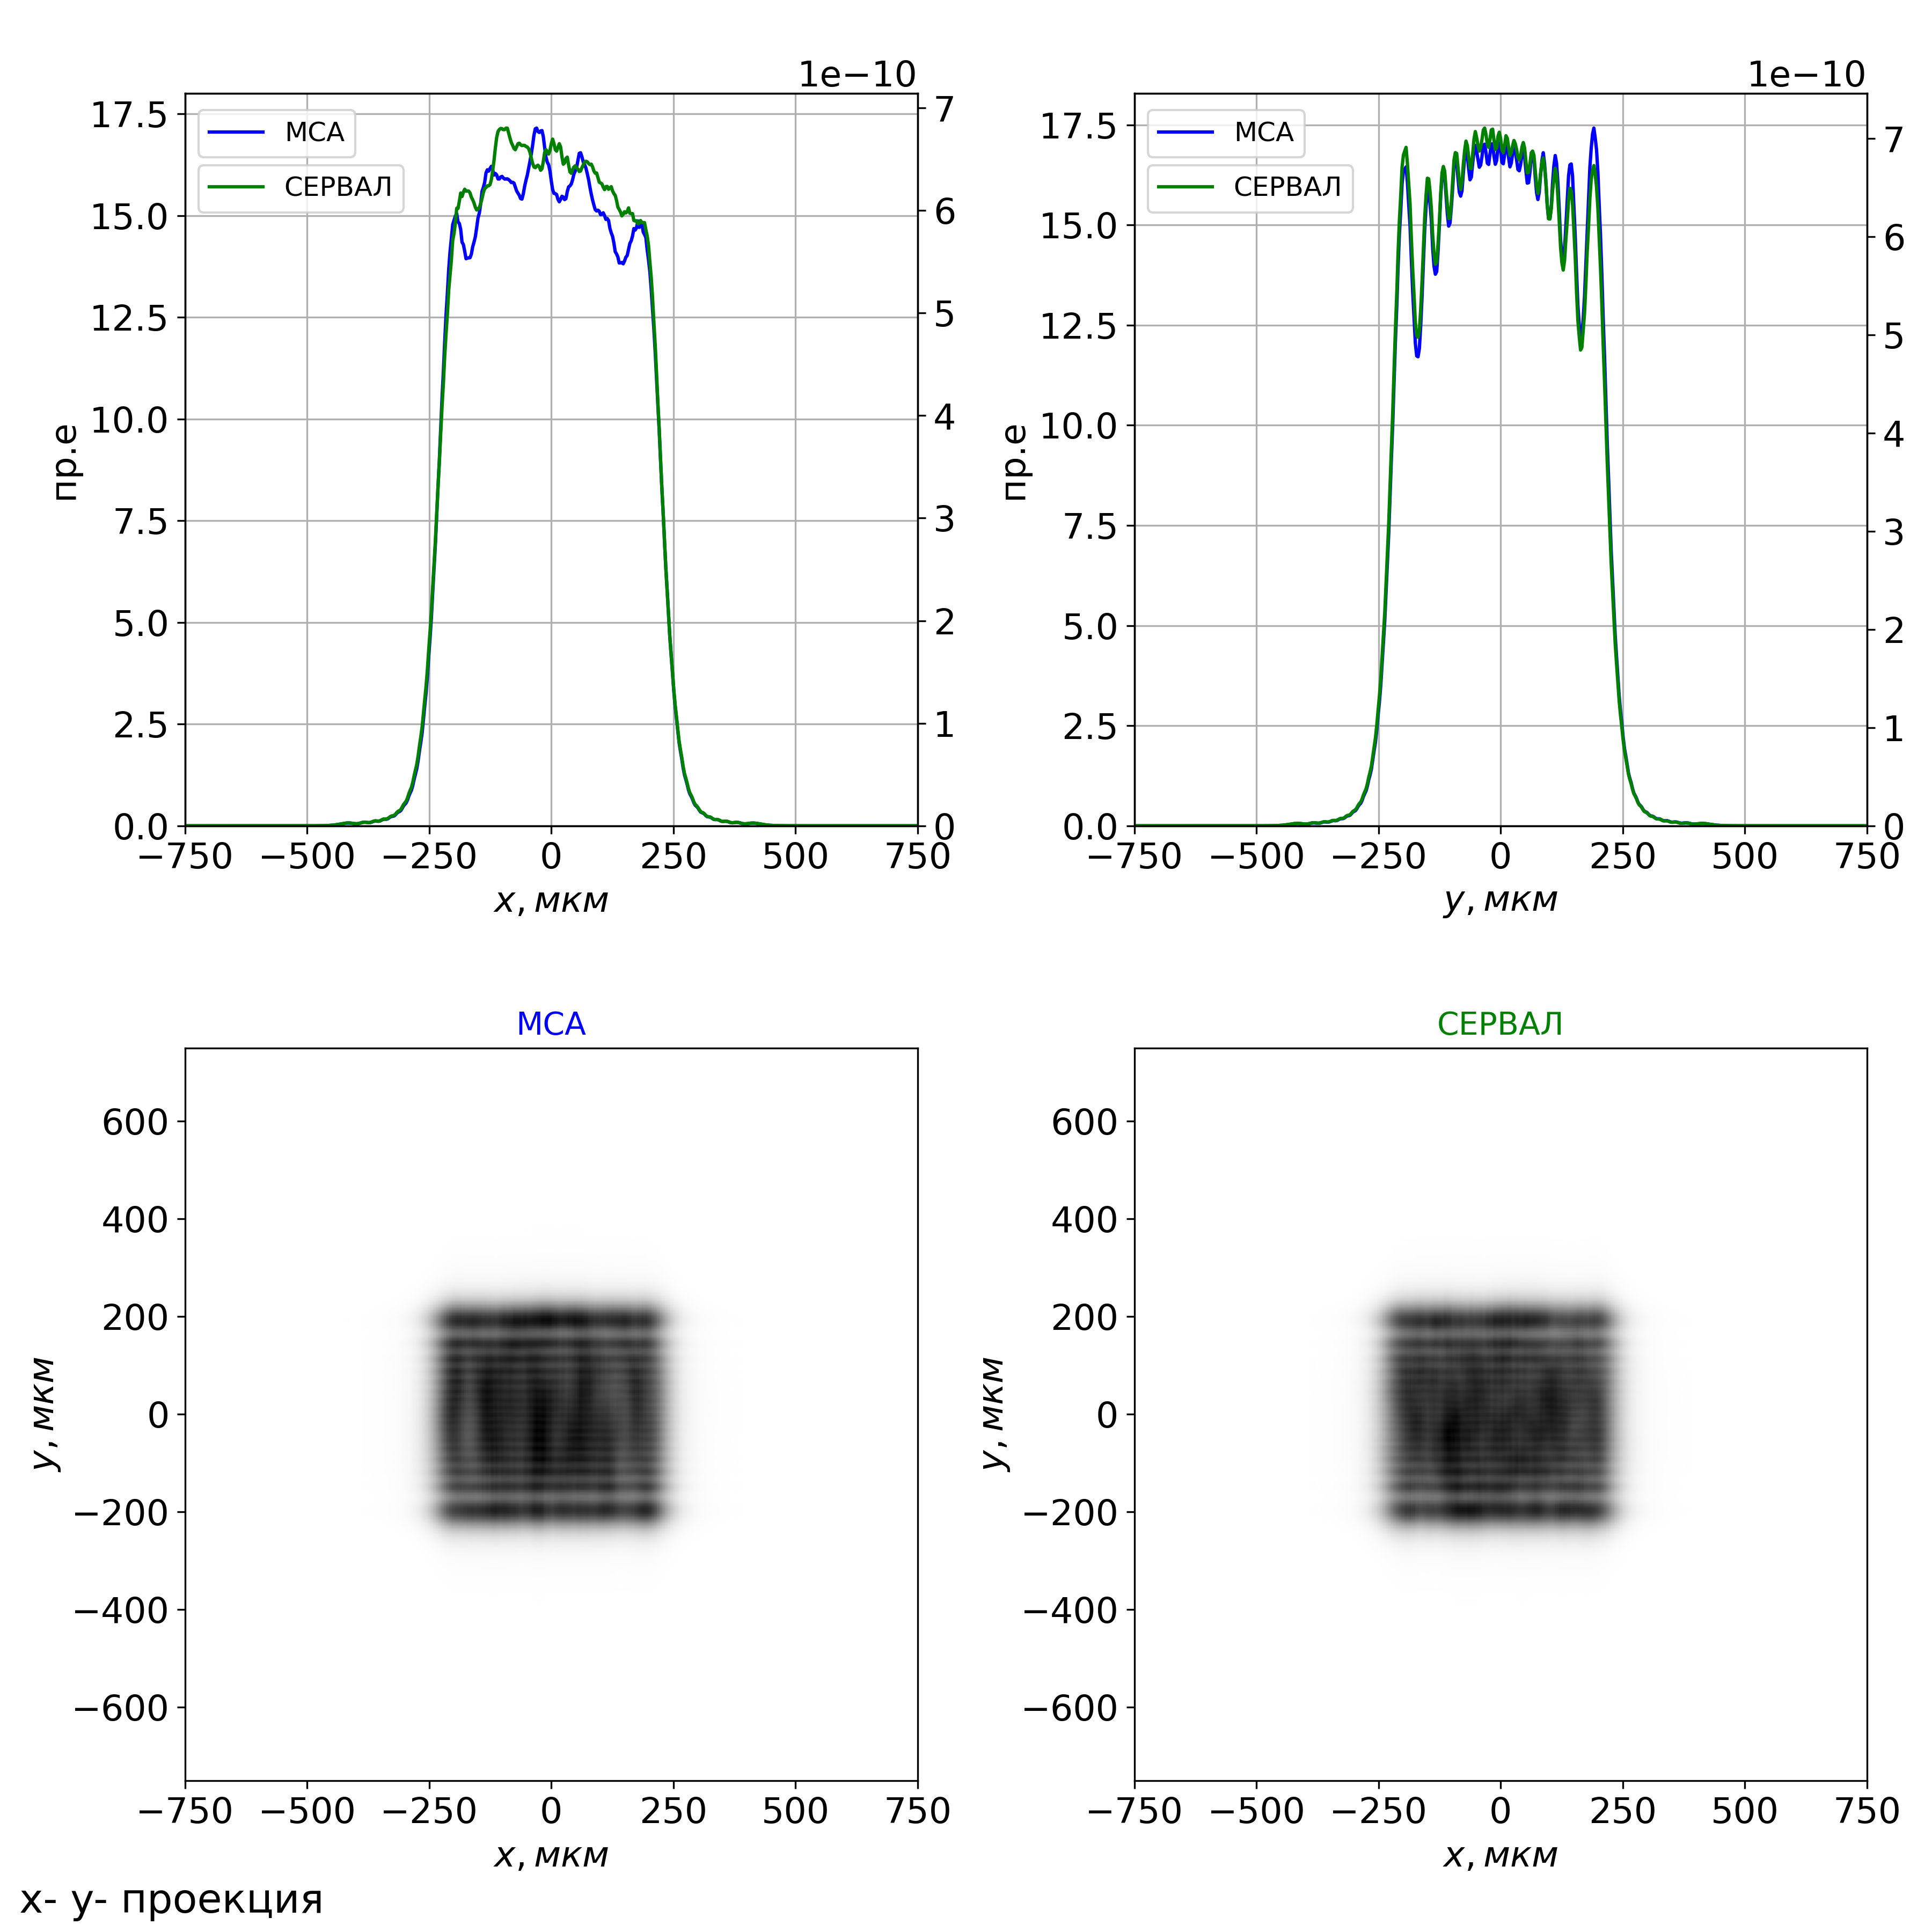
\includegraphics[width=0.99\linewidth]{2-far_zone_12_5_m_after_aperture3.80E-05_um_4.68E-06_um_2.50E-05_urad_2.00E-05_urad_example_beamline.png}
	\caption{\rr{$MCA_x, СЕРВАЛ_x = 453$ мкм, $MCA_x, СЕРВАЛ_x = 445, 442$ мкм}}
	\label{fig:focusing_system_after_aperture}
\end{figure}
\noindent Дифракционные картины отличаются для каждого из направлений, для вертикального дифракционные пики более выраженные ввиду большей длины когерентности, для горизонтального направления заметен только первый дифракционный максимум, что говорит о заметно меньшей степени когерентности.

Распределение поля в фокальной плоскости приведено на Рис.~\ref{fig:focusing_system_in_focus}.
\begin{figure}[H] 
	\centering 	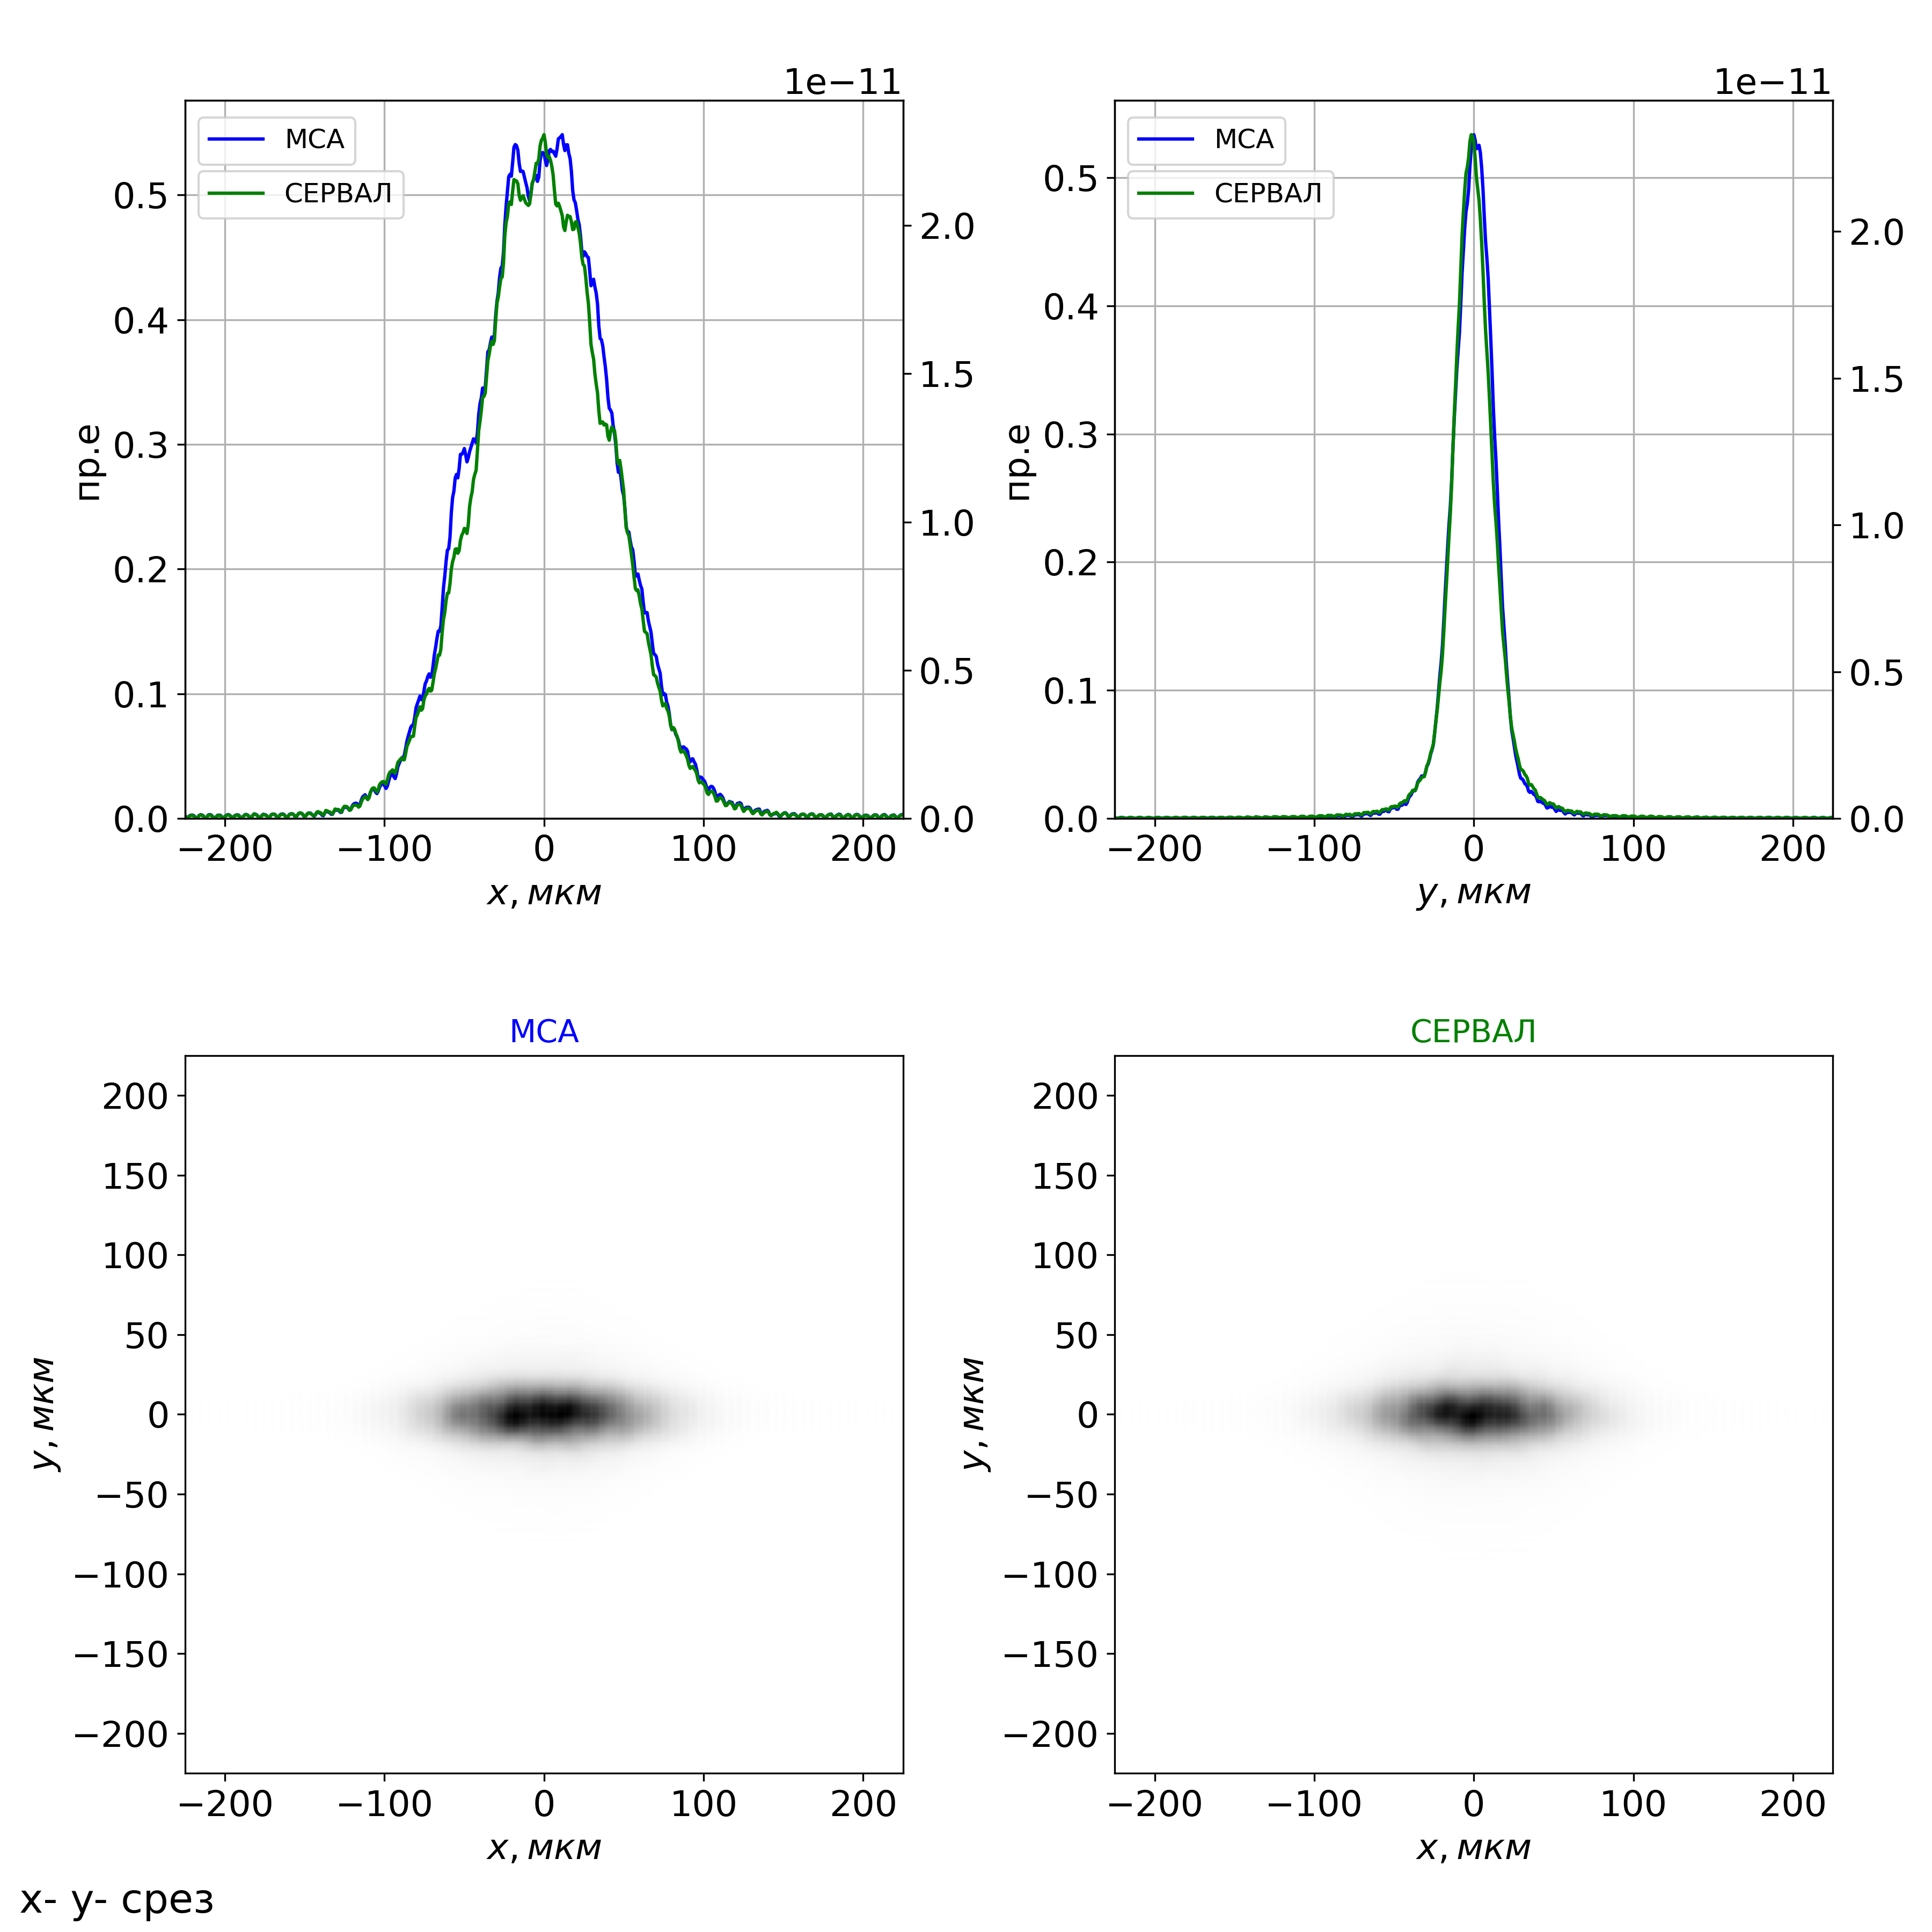
\includegraphics[width=0.99\linewidth]{3-70_m_focal_plane3.80E-05_um_4.68E-06_um_2.50E-05_urad_2.00E-05_urad_example_beamline.png}
	\caption{Распределение излучения в фокусе \rr{$MCA_x, СЕРВАЛ_x = 100$ мкм, $MCA_x, СЕРВАЛ_x = 26$ мкм}}
	\label{fig:focusing_system_in_focus}
\end{figure}
\noindent Для моделирования было выбрано соотношение плеч фокусирующей системы -- $1:1$. В горизонтально направлении источник можно считать гауссовым с полной шириной на полувысоте $80$ мкм, после фокусировки мы видим уширение изображения до $100$ мкм, которое приходит из-за апертуры и намного меньшее уширение в вертикальном направлении до $26$ мкм при истинном размере источника $24$ мкм. По критерию Релея $\theta_{diff} = 1.22 \lambda / D$, где $D$ размер апертуры, -- дифракционный предел для обоих направлений $0.7$ мкрад при видимом размере источника для горизонтального направления $3.2$ мкрад и $0.96$ мкрад -- для вертикального. Видно, что для горизонтального направления та же апертура будет вносить больший вклад в увеличение размера фокусного пятна.
\rr{заключение}
\section{Интерференционный эксперимент}
Чтобы наглядно продемонстрировать эффекты, связанные с частичной когерентностью, показательно будет провести классический опыт Юнга (двухщелевой интерферометр Юнга). Ниже на Рис.~\ref{fig:x_field_before_slit} и~\ref{fig:x_corr_before_slit} опять же приведён размер излучения на $25$ м от источника излучения и распределение корреляционной функции в увеличенном масштабе с наложенными щелями. Щели на рисунках обозначены зелёным цветом -- с межщелевым зазором $75$ мкм, красным -- $150$ мкм и оранжевым $300$ мкм, при характерном размере корреляционной функции полной шириной на половине высоты (ПШПВ) $87 \times 320$ $\textup{мкм}^2$. 
\begin{figure}[H]
	\centering
	\begin{minipage}{0.33\textwidth}
		\centering
		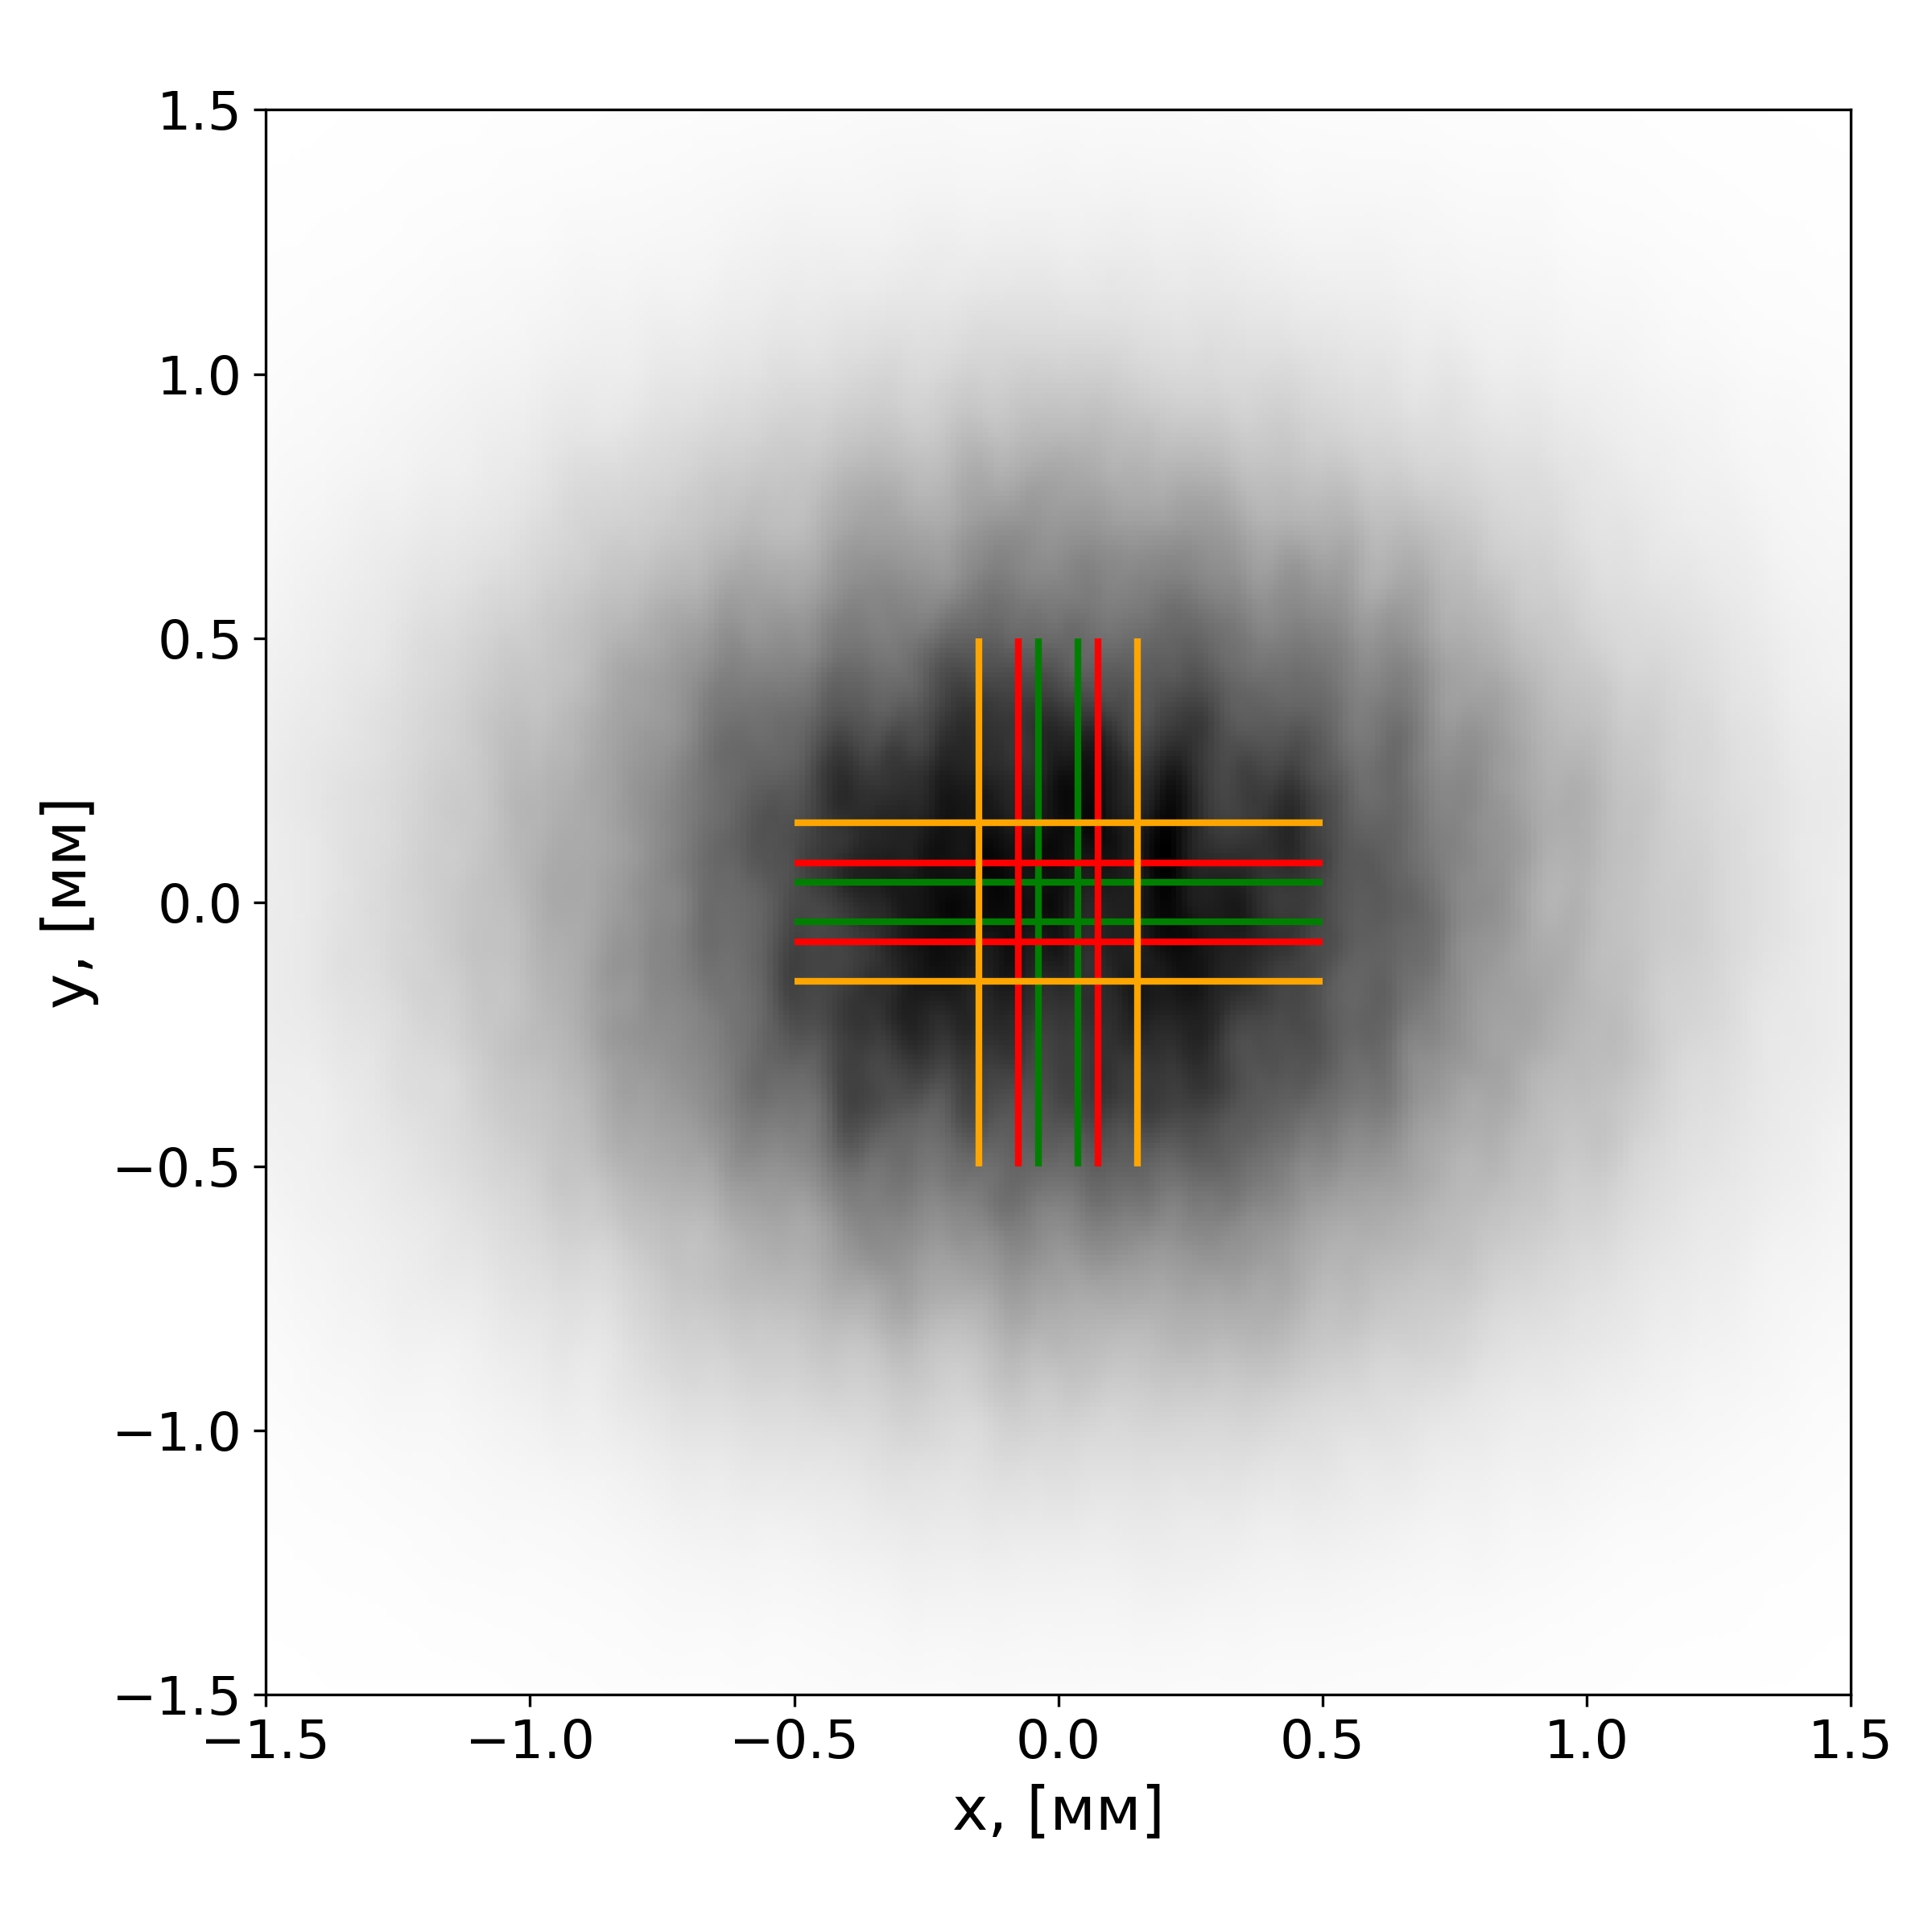
\includegraphics[width=1\linewidth]{field_before_slit.png}
		\caption{Размер излучения на $25$ м от источника с щелями, обозначенными цветными полосками  \rr{убрать горизонтальные полоски}}
		\label{fig:x_field_before_slit}
	\end{minipage}
	\begin{minipage}{0.33\textwidth}
		\centering
		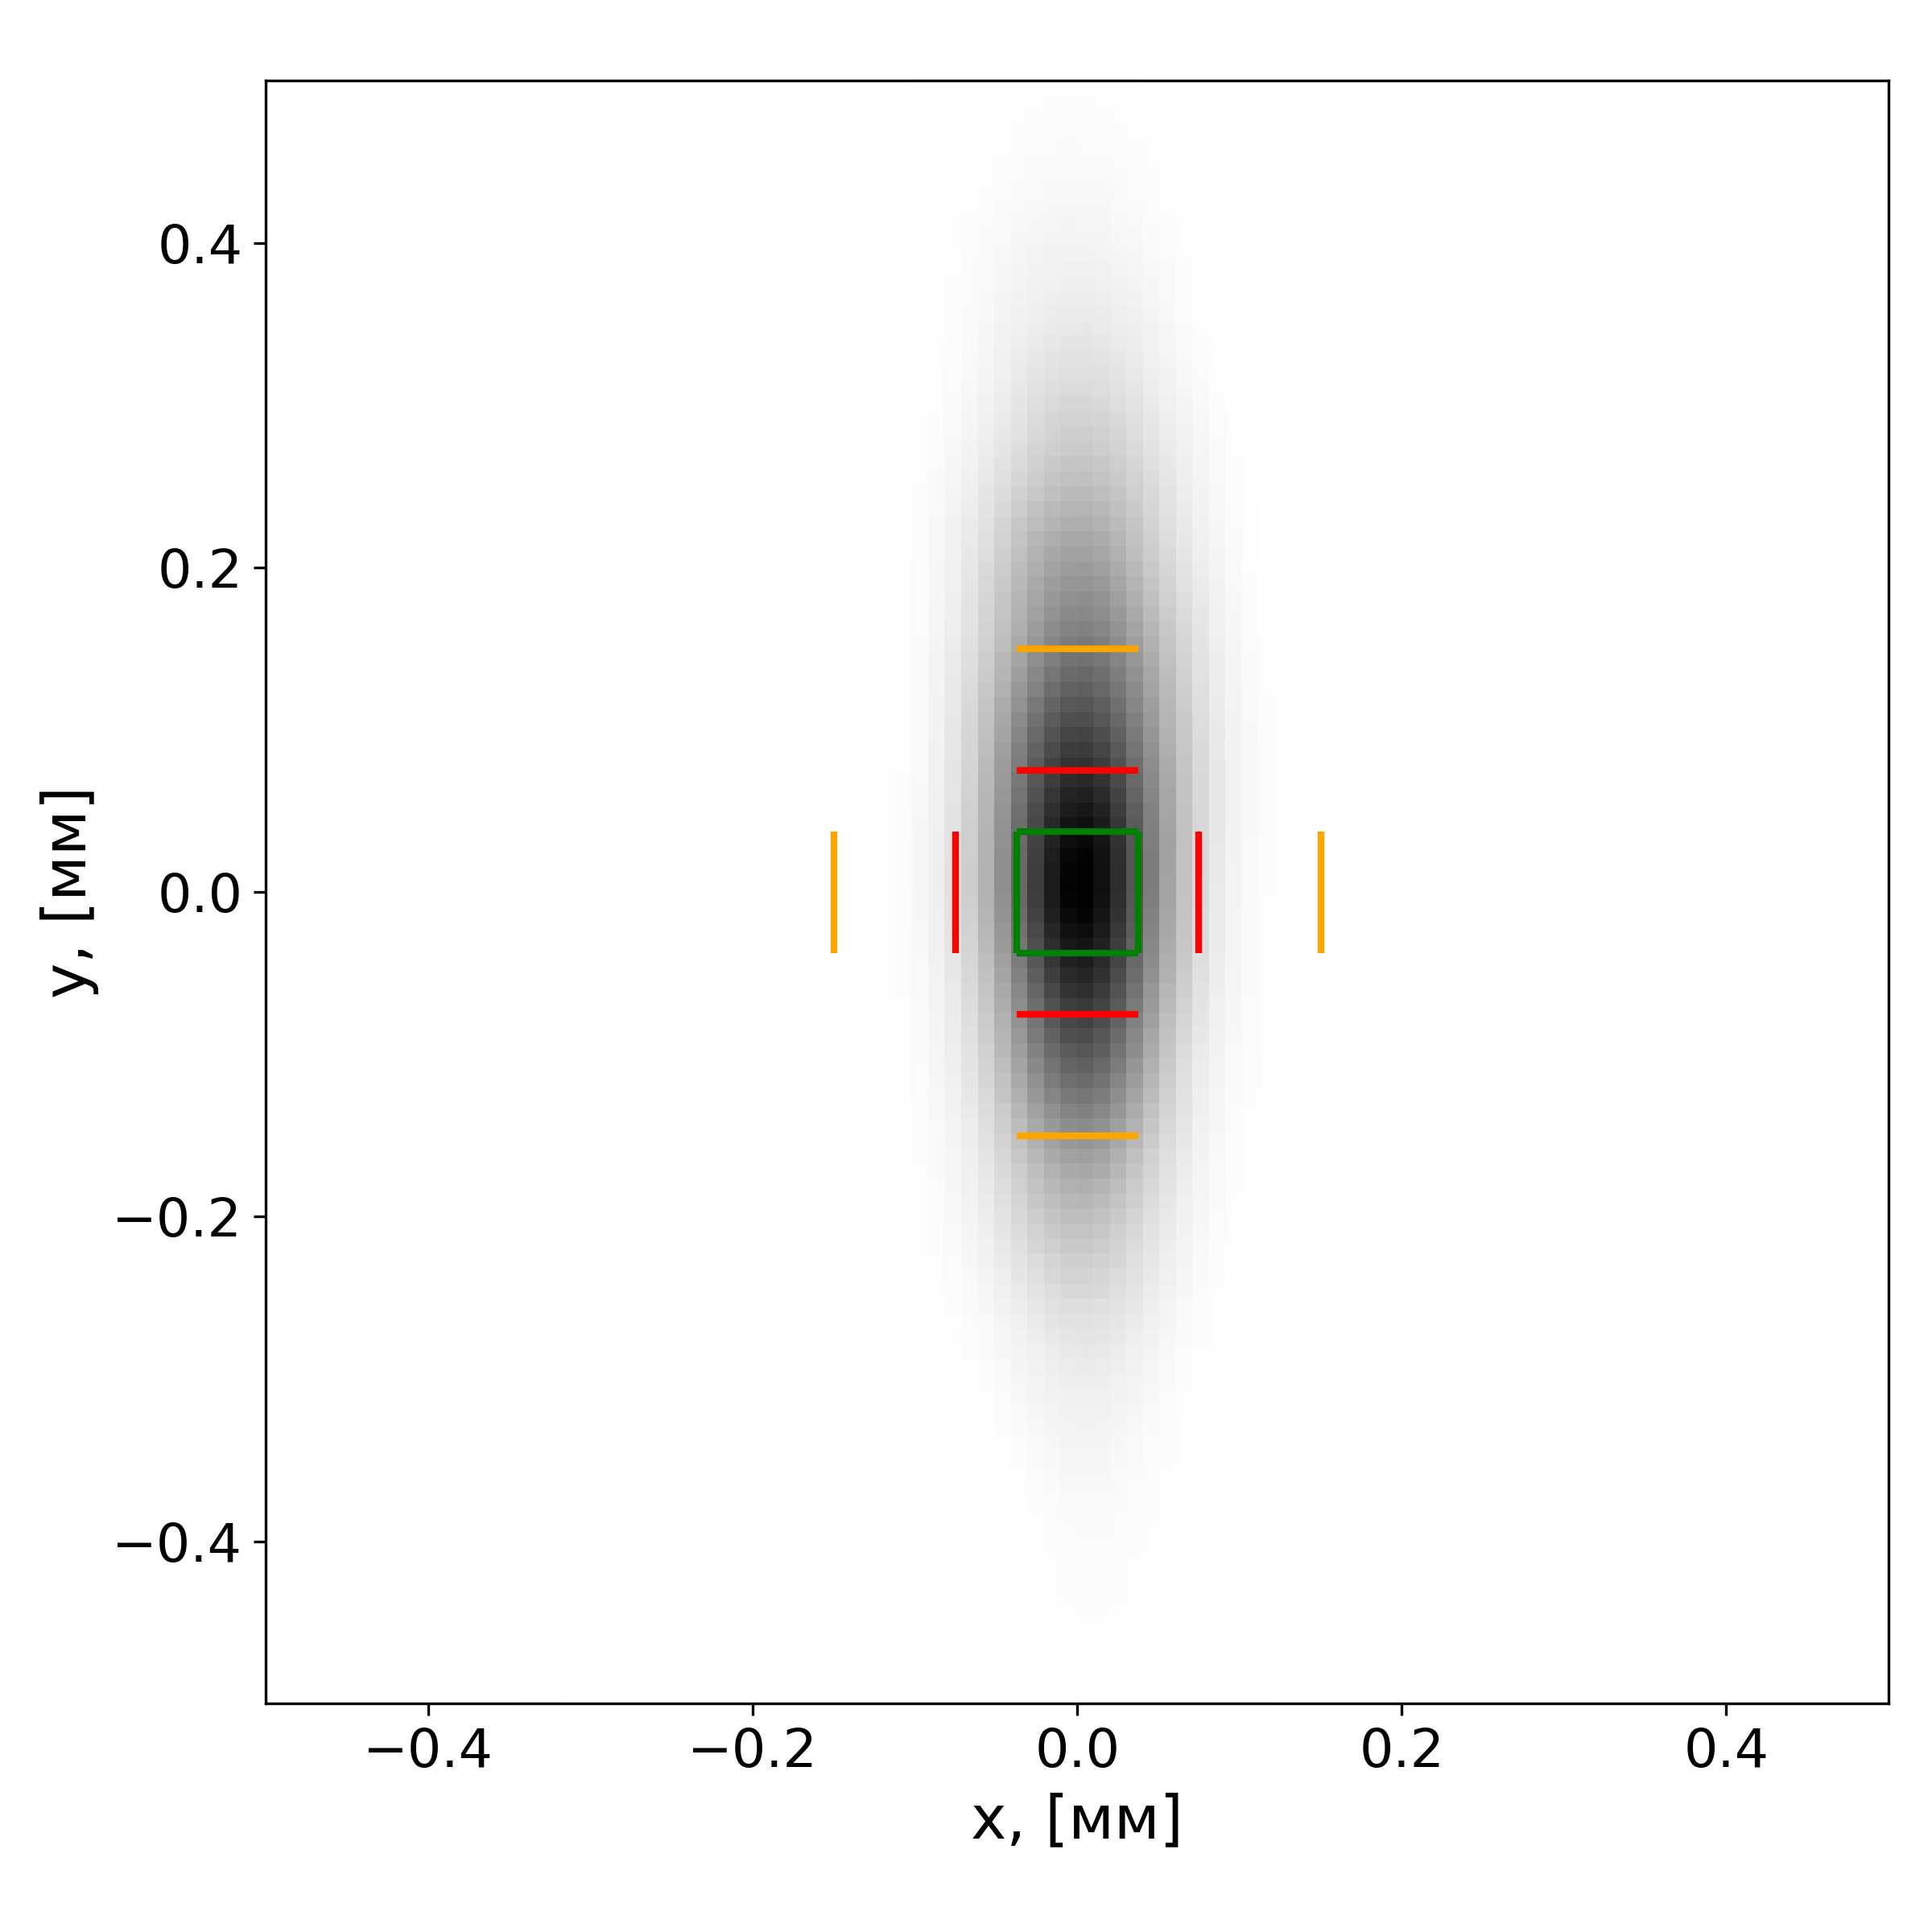
\includegraphics[width=1\linewidth]{corr_before_slit.png}
		\caption{Пятно когерентности на $25$ м от источника с щелями, обозначенными цветными полосками \rr{убрать горизонтальные полоски}}
		\label{fig:x_corr_before_slit}
	\end{minipage}\hfill
\end{figure}
\noindent Для начала продемонстрируем интерференционную картину отдельно от каждой из реализации и получившееся усреднённое по реализациям изображение, представленные на Рис.~\ref{fig:double slit experiment} для вертикального расположения щелей с щелевым зазором $75$ мкм.
\begin{figure}[H] 
	\centering 	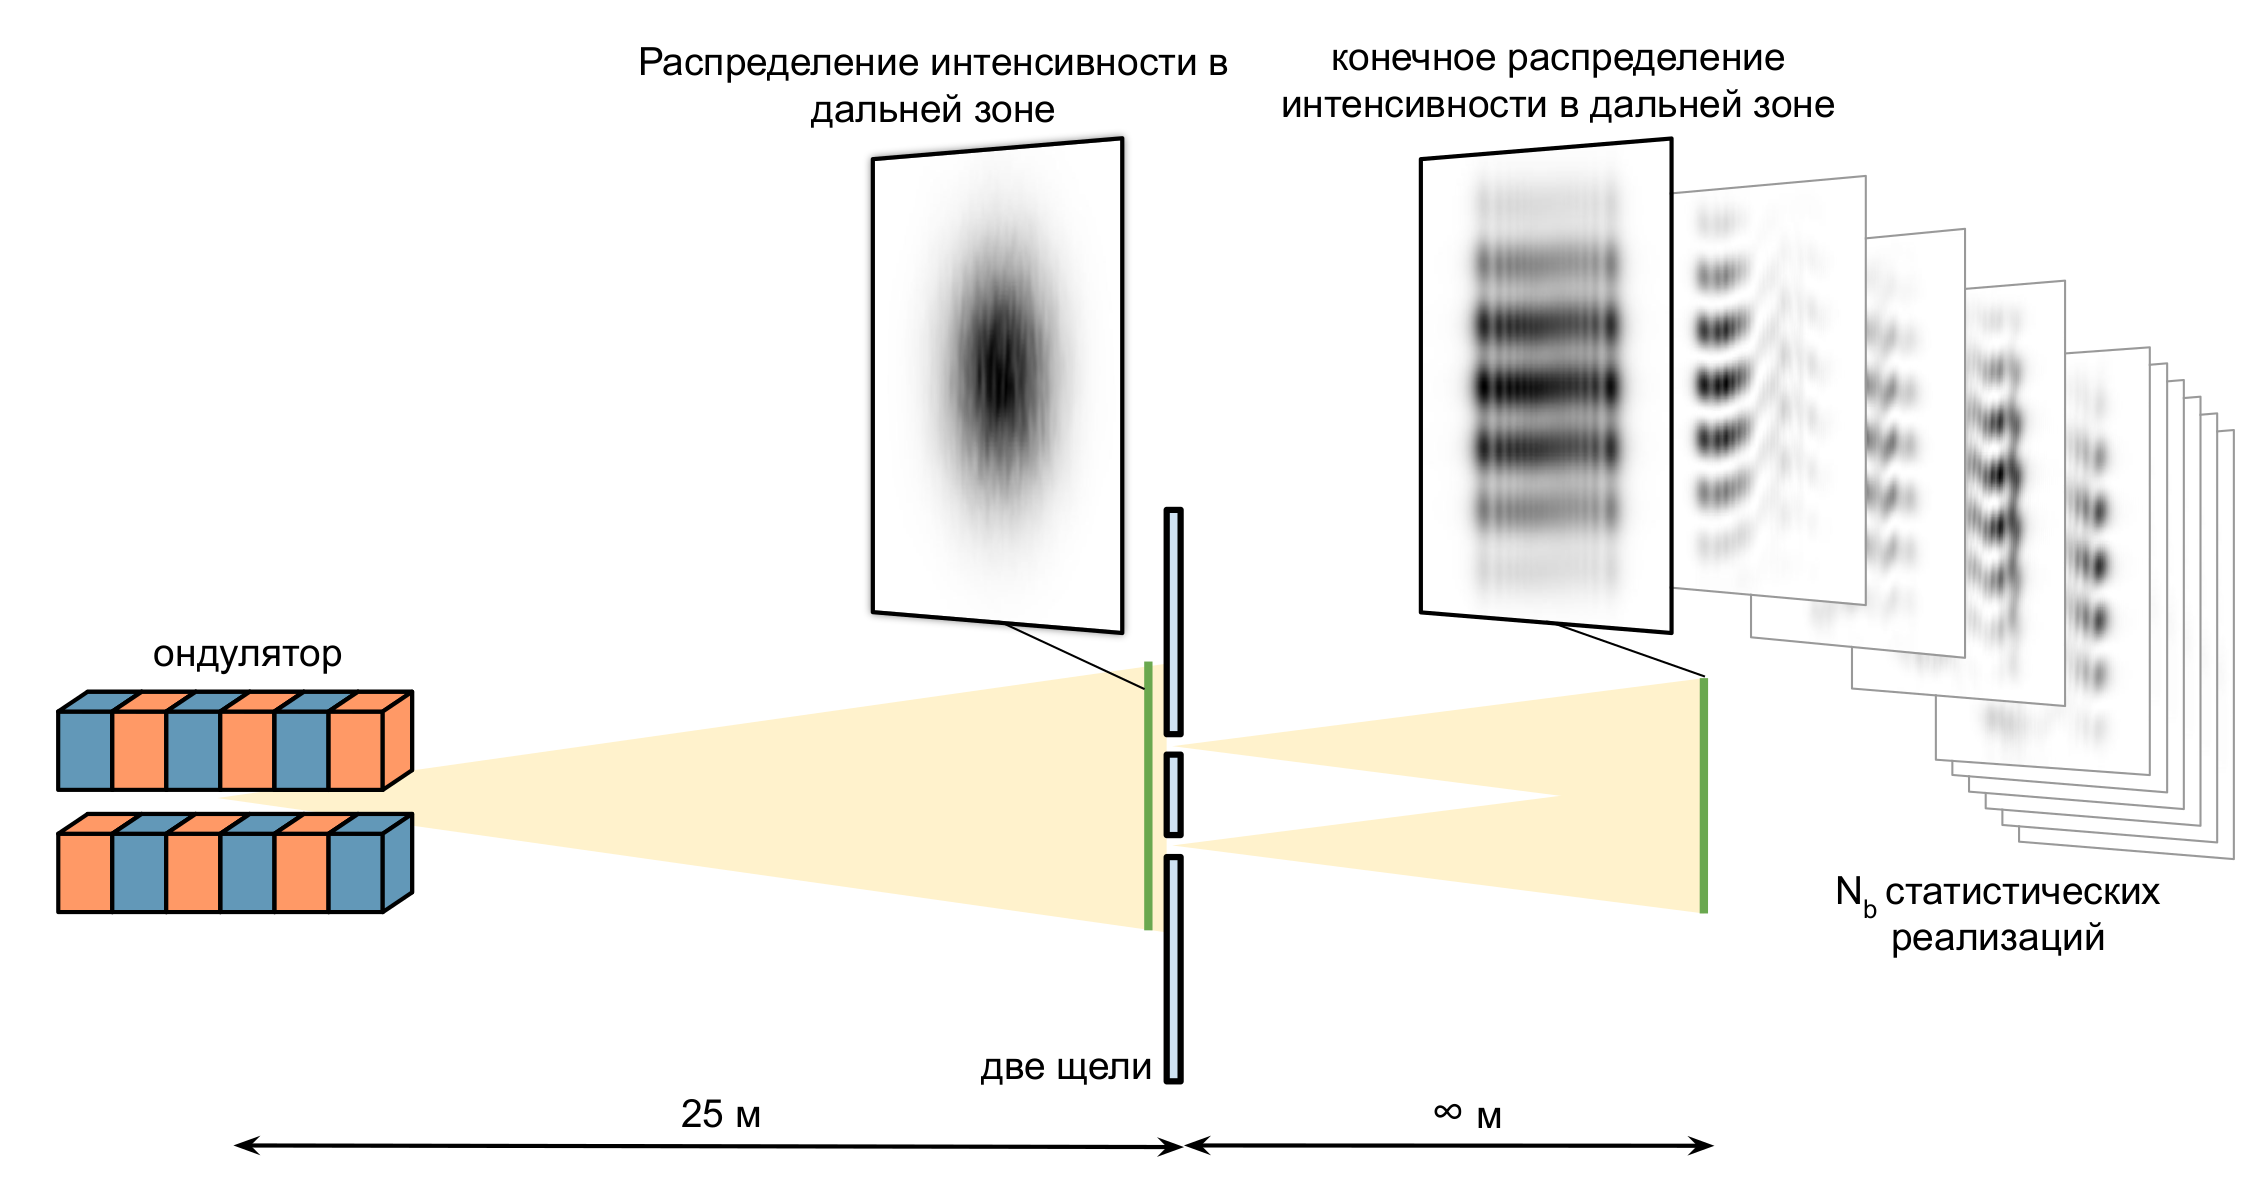
\includegraphics[width=0.99\linewidth]{double_slit_scheme.png}
	\caption{Схема двухщелевого эксперимента. После щелей -- интерферограмма усреднённая по 400 реализациям, а за ней интерферограммы для отдельных реализаций из этого статистического набора набора. Интерферограммы приведены в k-пространства сразу за щелями. Примечательно, что видность каждой из реализаций равна единице, но при усреднение по многим реализациям видность падает ввиду наличия частичной когерентности излучения]}
	\label{fig:double slit experiment}
\end{figure}
\noindent Дело в том, что «Хотя видность любой из этих отдельны интерферограмм соответствует значение\footnote{$\mu_{12}$ -- комплексный коэффициент когерентности, соответствующий $g^{(1)}$ в настоящей работе} $|\mu_{12}| = 1$, видность суперпозиции интерферограмм, вообще говоря, будет иной, поскольку фазы отдельных компонент будут изменяться от реализации к реализации. Таким образом, интерферограмма, усреднённая по ансамблю, вообще говоря, даст значения $|\mu_{12}|$, весьма отличные от единицы.», -- Дж. Гудмен, «Статистическая оптика», издательство «Мир», 1988, стр. $332-333$ или зарубежное издание~\cite{goodman_statistical_2015}.

Теперь можно представить усреднённые по реализациям интерферограммы для различных межщелевых расстояний, представленные на Рис.~\ref{fig:x_slits_75},~\ref{fig:x_slits_150},~\ref{fig:x_slits_300}. Указанные картины представлены для вертикального расположения щелей.
\begin{figure}[H]
	\centering
	\begin{minipage}{0.33\textwidth}
		\centering
		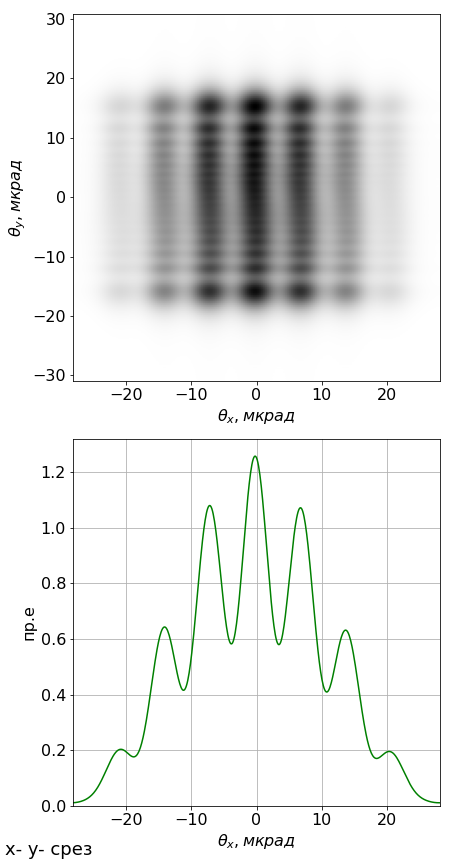
\includegraphics[width=1\linewidth]{x_slits_width_3e-05_separation_7.5e-05_.png}
		\caption{$75$ мкм}
		\label{fig:x_slits_75}
	\end{minipage}
	\begin{minipage}{0.33\textwidth}
		\centering
		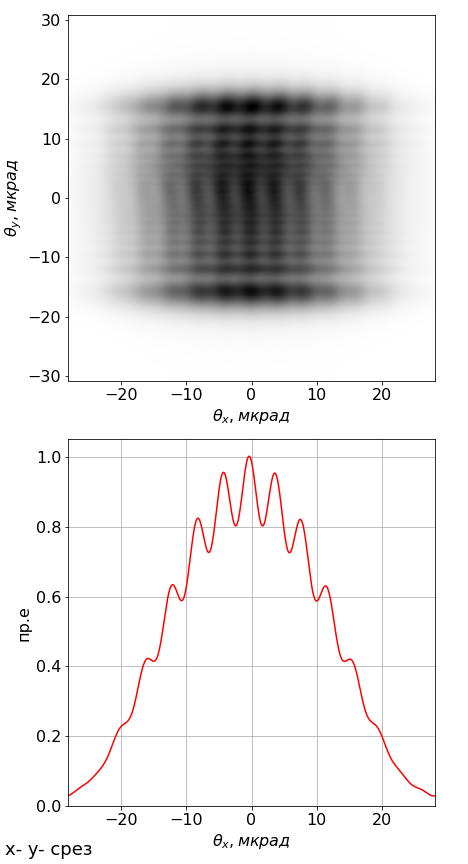
\includegraphics[width=1\linewidth]{x_slits_width_3e-05_separation_0.00015_.png}
		\caption{$150$ мкм}
		\label{fig:x_slits_150}
	\end{minipage}\hfill
	\begin{minipage}{0.33\textwidth}
		\centering
		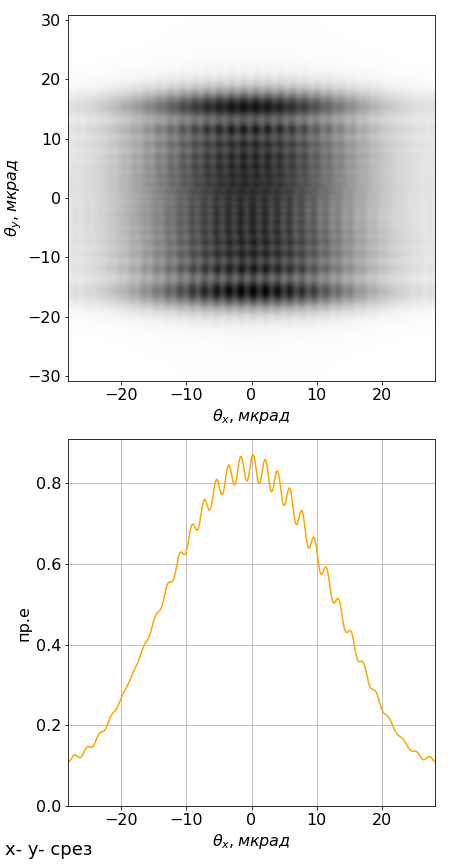
\includegraphics[width=1\linewidth]{x_slits_width_3e-05_separation_0.0003_.png}
		\caption{$300$ мкм}
		\label{fig:x_slits_300}
	\end{minipage}\hfill
\end{figure}
Примечательно заметить, что эти интерференционные картины представлены в $k$-пространстве или, другими словами, представлены в дальней зоне на достаточном расстоянии $z$ от щелей\footnote{так же именно такое изображение получится, если сразу за щелями поставить линзу, в фокусе будет соответствующая дифракционная картина}. Ещё одна особенность получившихся изображений: щели имеют конечный, в данном случае, горизонтальны размер равный $1$ мм, именно поэтому в вертикальном направлении на Рис.~\ref{fig:x_slits_75},~\ref{fig:x_slits_150},~\ref{fig:x_slits_300} видны характерные дифракционные картины от плоскости.

Аналогичные интерферограммы построены для вертикального направления, в котором излучение обладает большей когерентностью. Щели в данном случае ориентированны горизонтально.
\begin{figure}[H]
	\centering
	\begin{minipage}{0.33\textwidth}
		\centering
		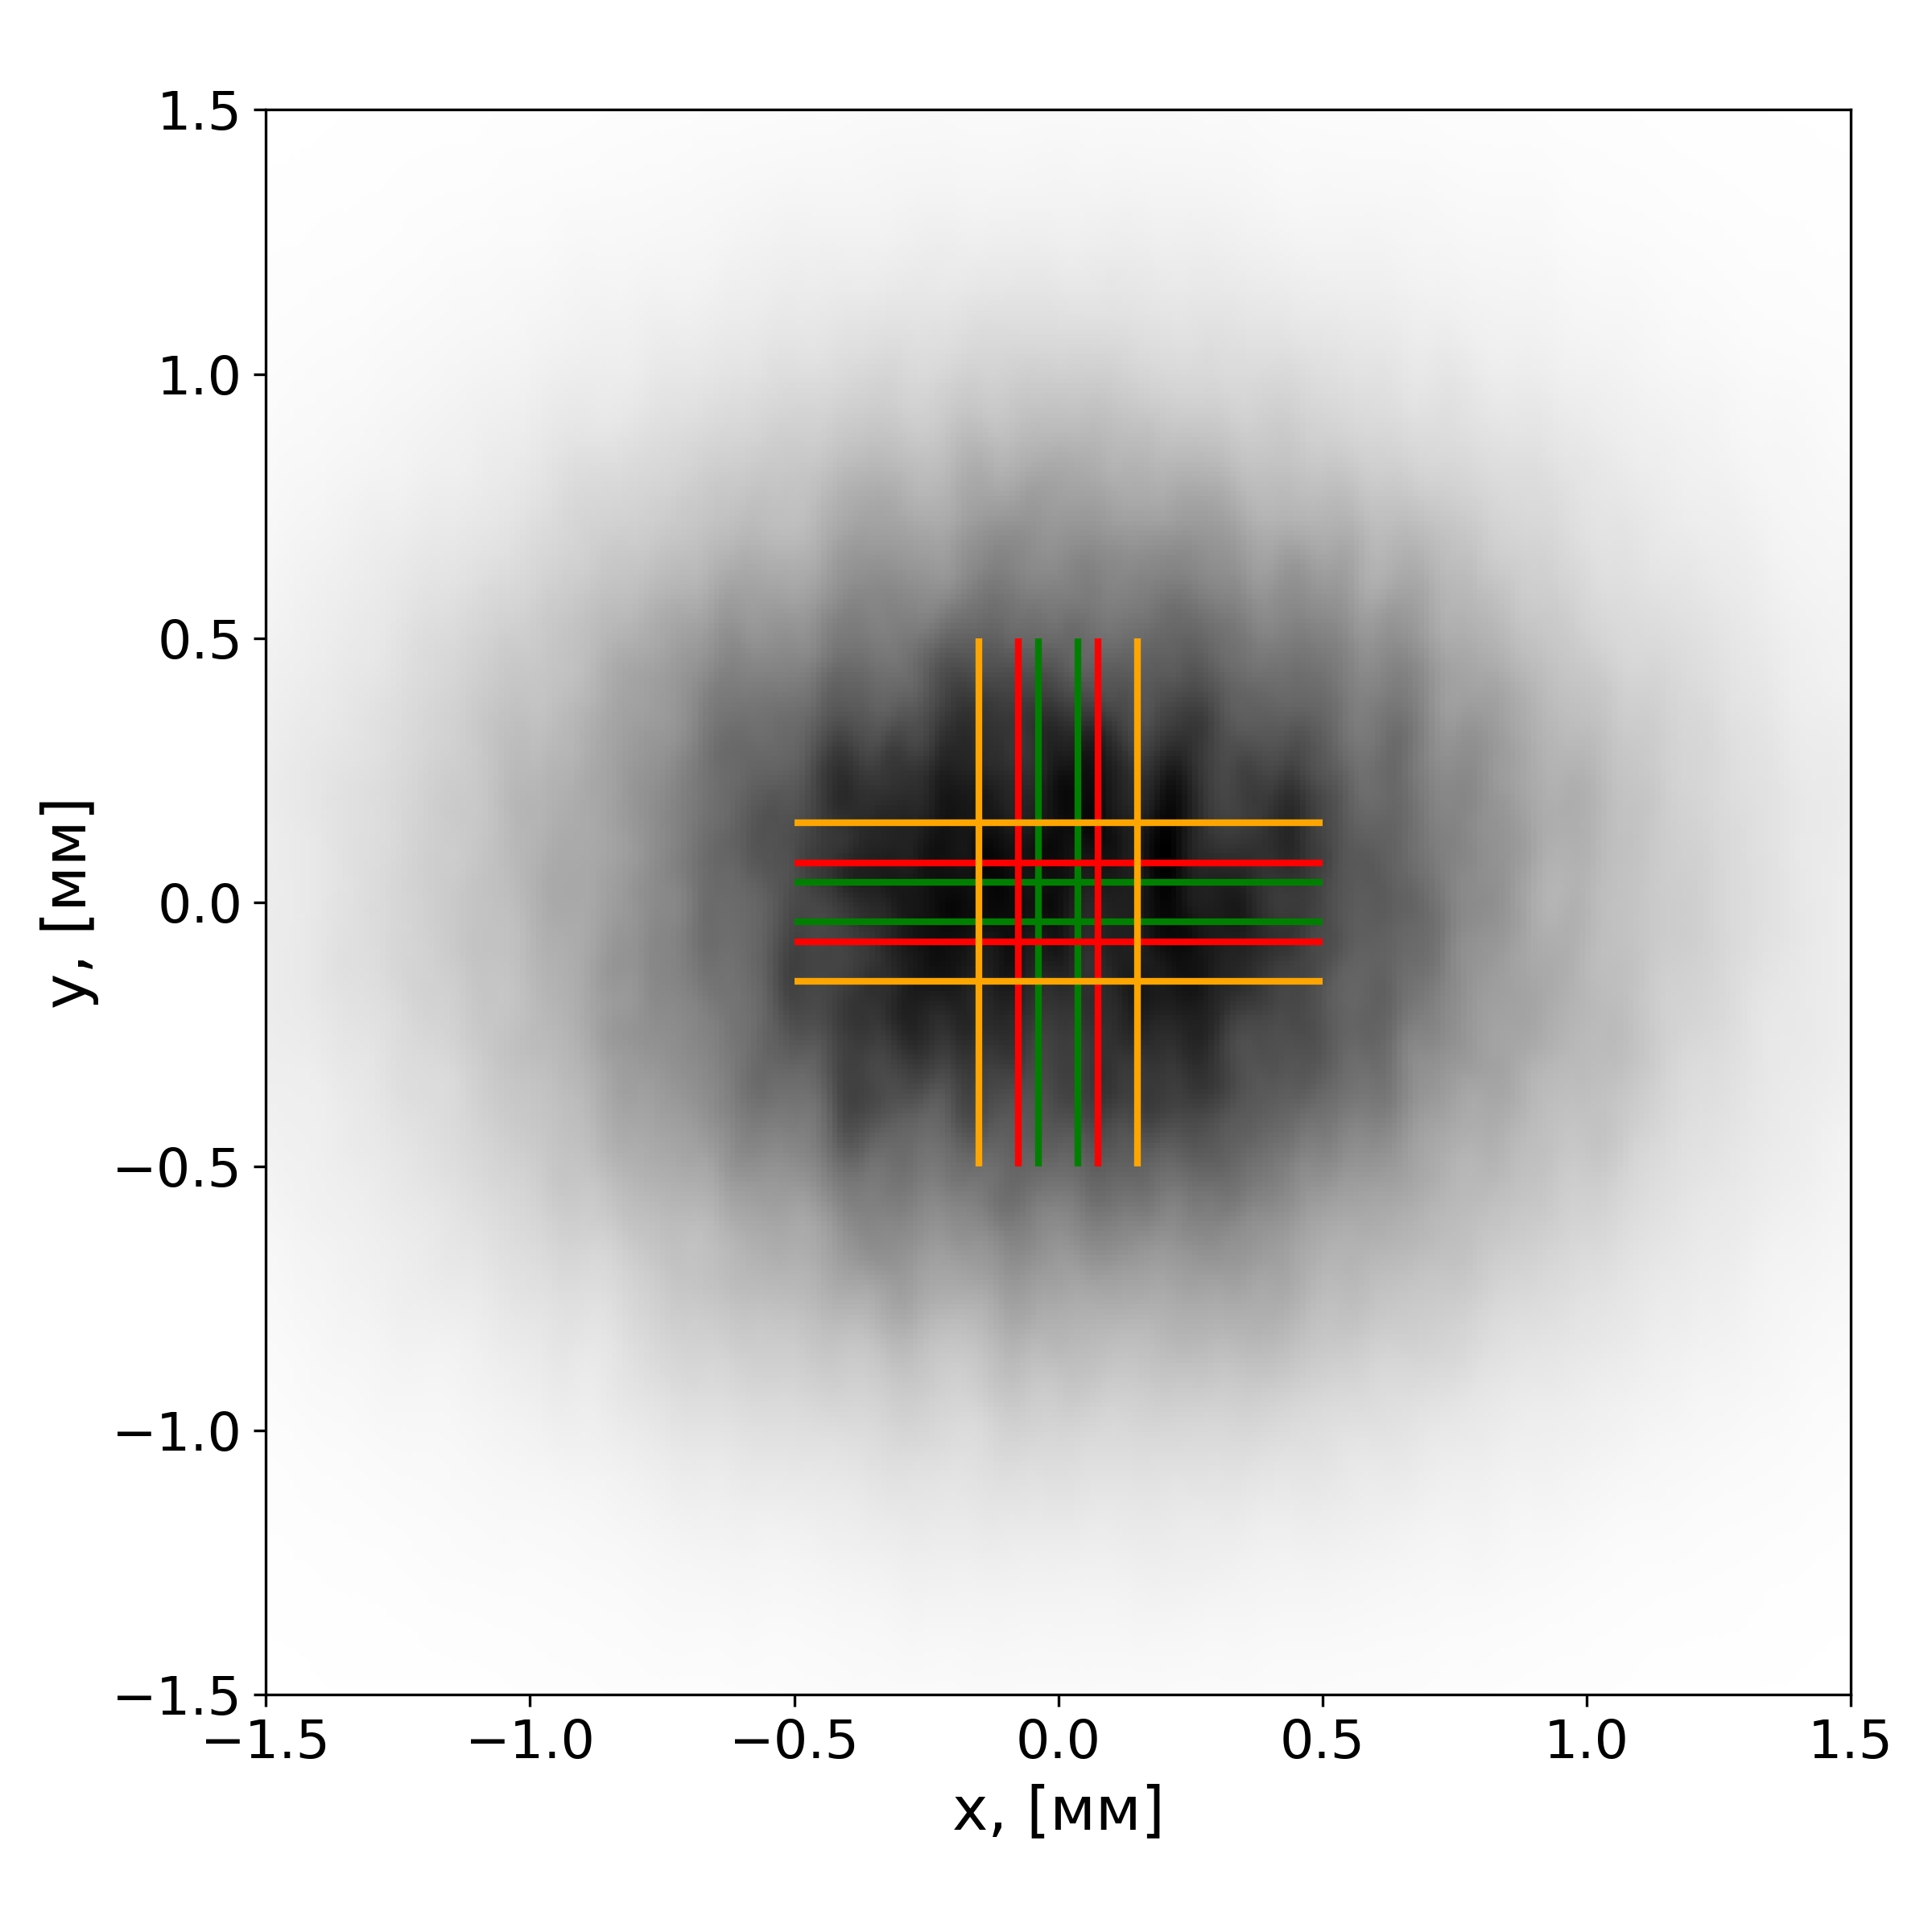
\includegraphics[width=1\linewidth]{field_before_slit.png}
		\caption{\rr{убрать вертикальные полоски}}
		\label{fig:y_field_before_slit}
	\end{minipage}
	\begin{minipage}{0.33\textwidth}
		\centering
		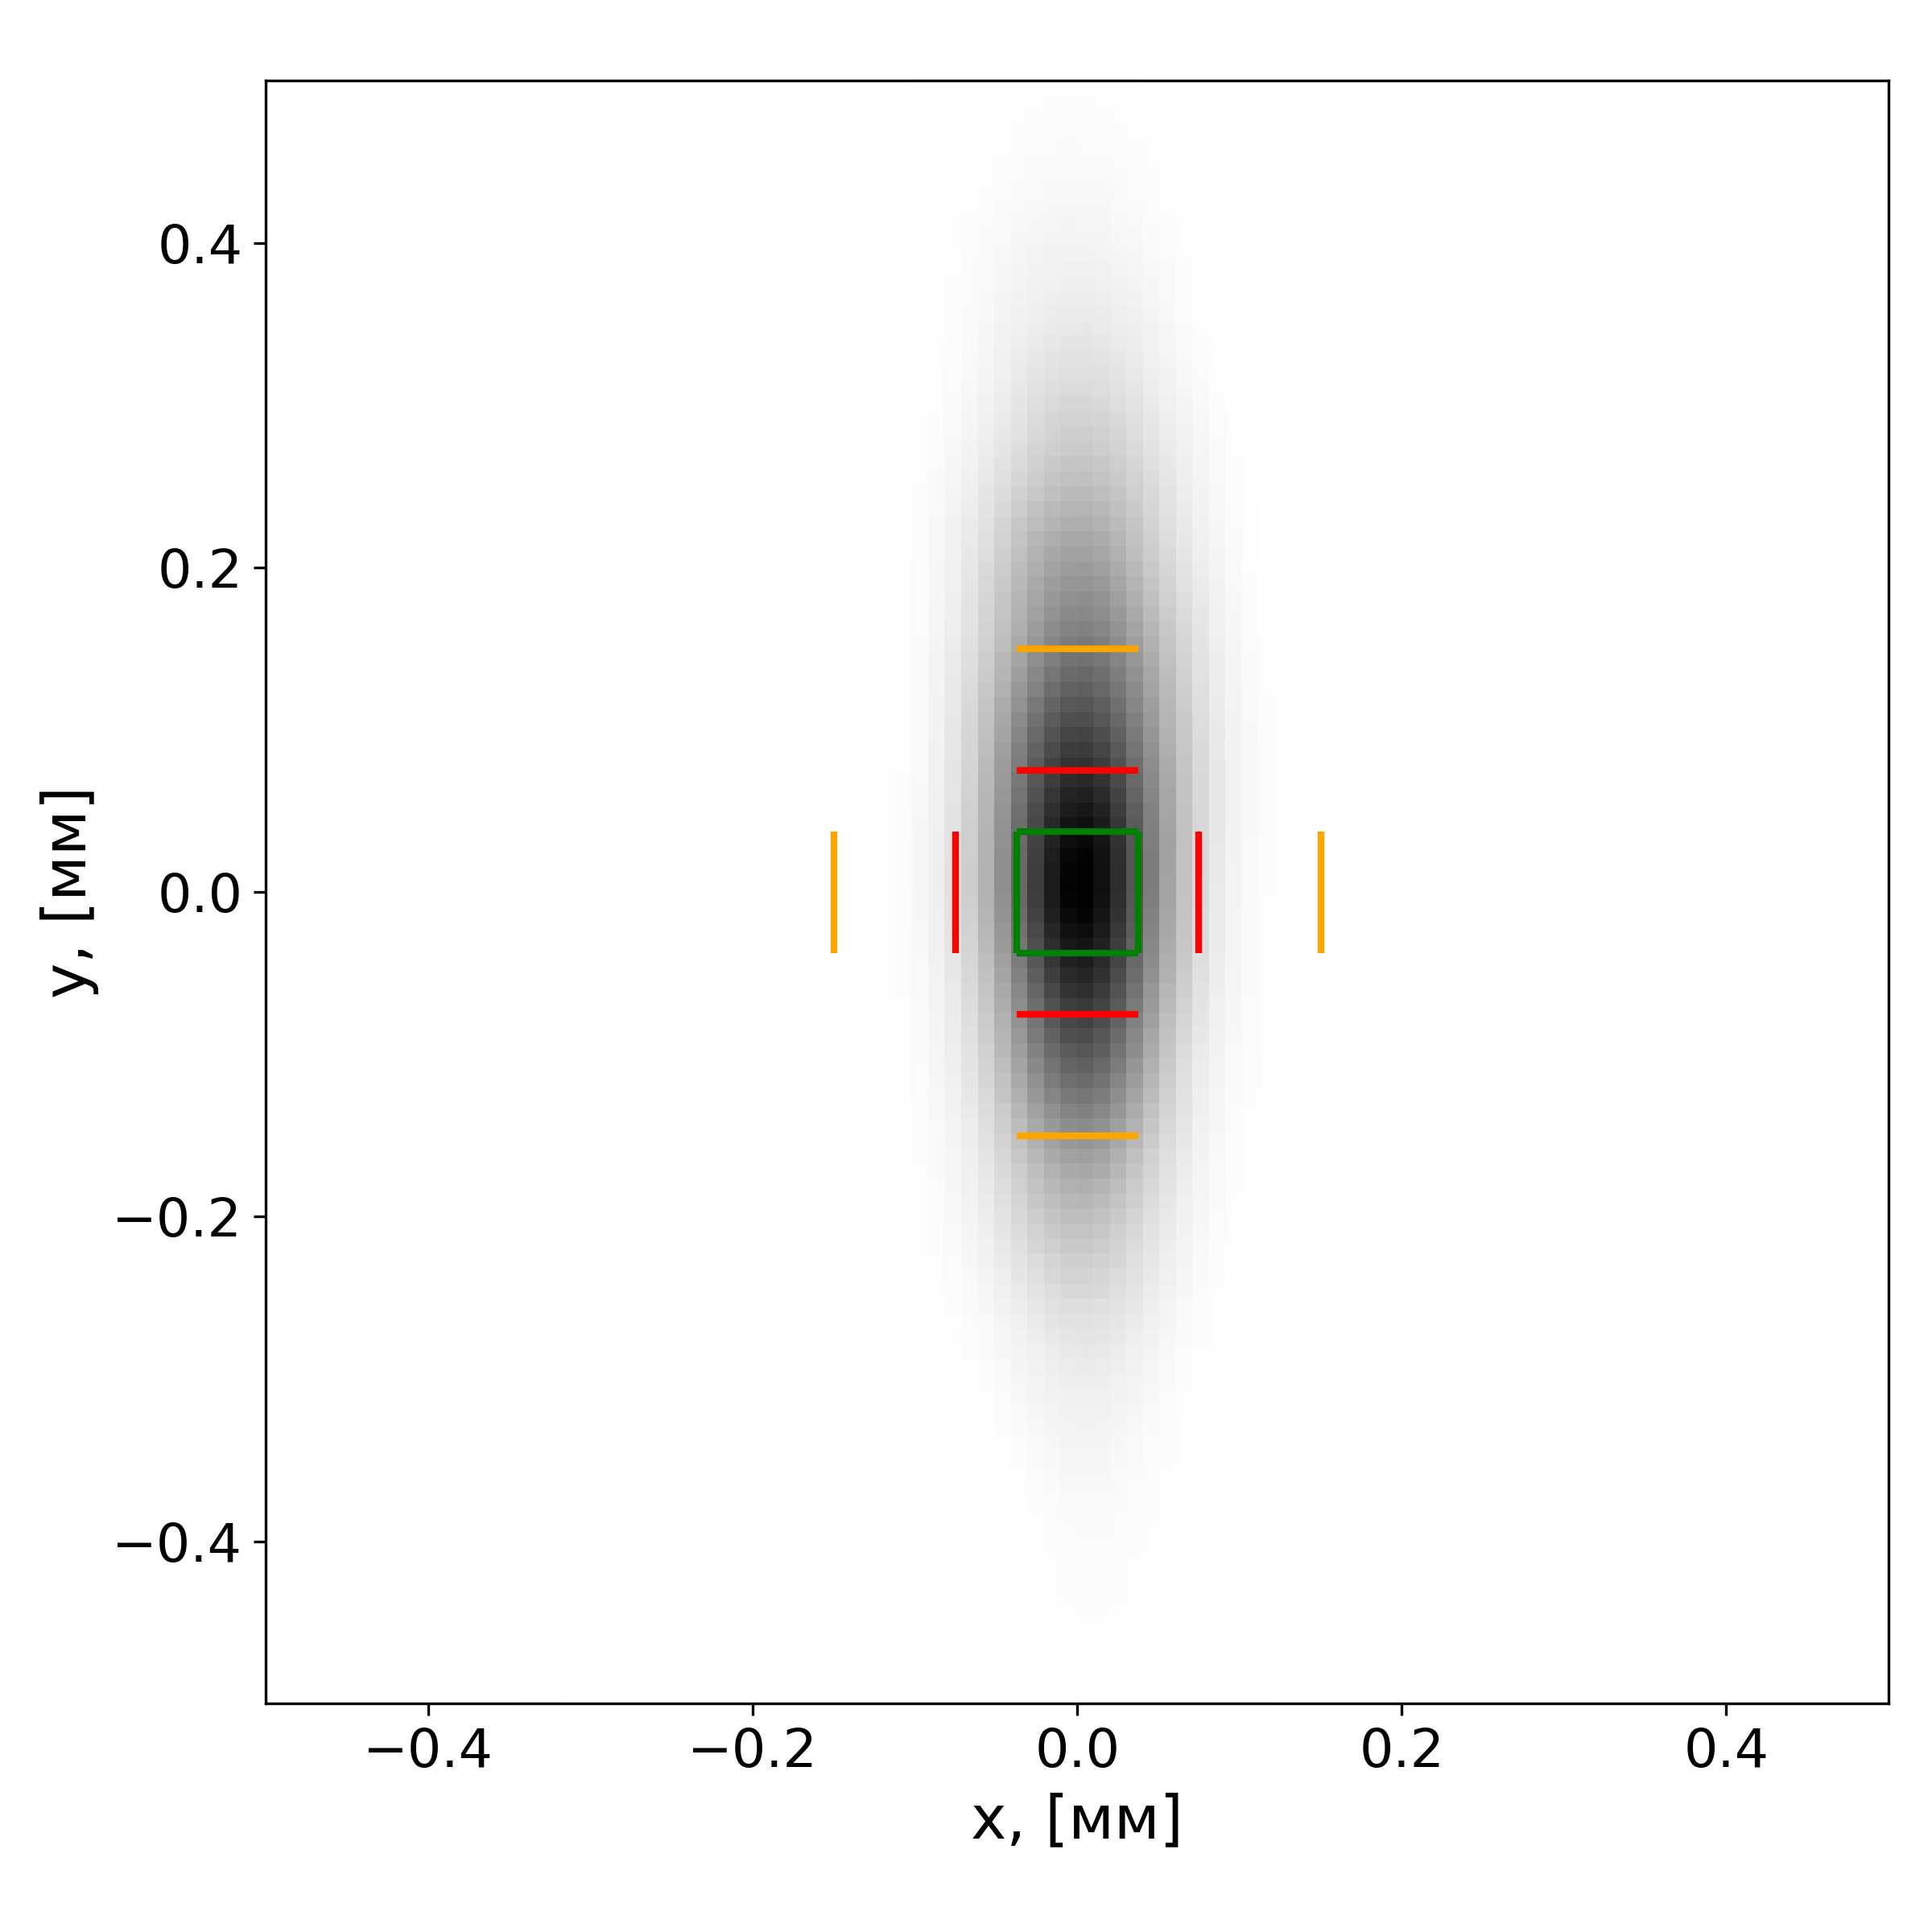
\includegraphics[width=1\linewidth]{corr_before_slit.png}
		\caption{\rr{убрать вертикальные полоски}}
		\label{fig:y_corr_before_slit}
	\end{minipage}\hfill
\end{figure}

\begin{figure}[H]
	\centering
	\begin{minipage}{0.33\textwidth}
		\centering
		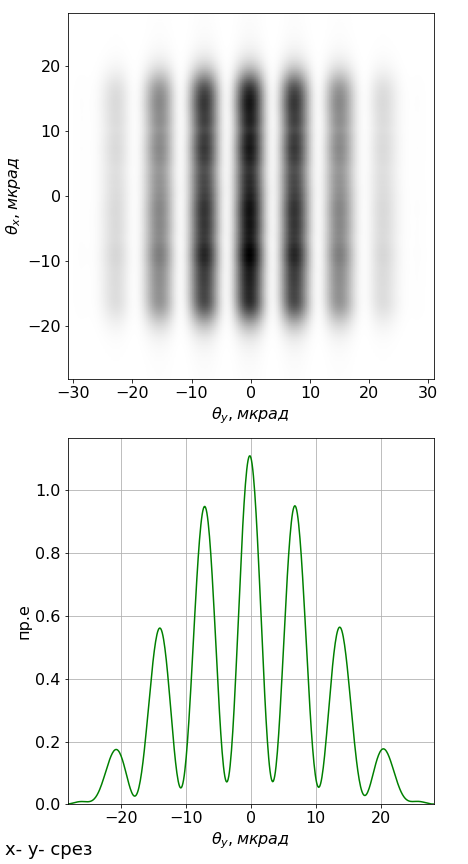
\includegraphics[width=1\linewidth]{y_slits_width_3e-05_separation_7.5e-05_.png}
		\caption{$75$ мкм}
		\label{fig:y_slits_75}
	\end{minipage}
	\begin{minipage}{0.33\textwidth}
		\centering
		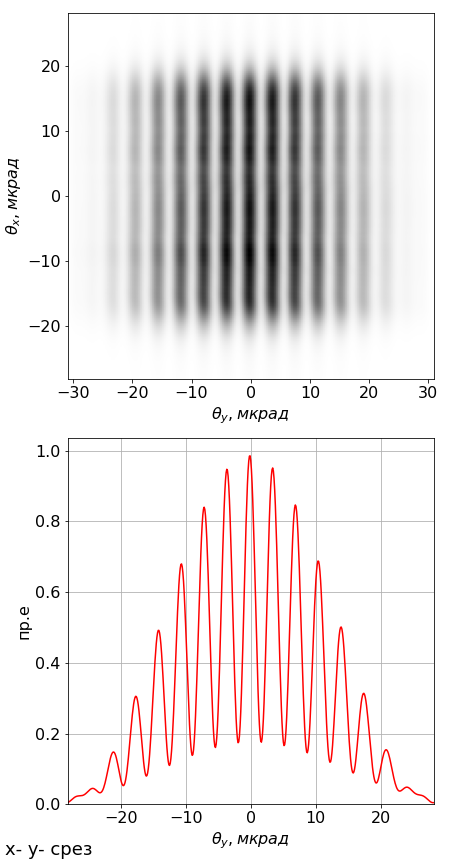
\includegraphics[width=1\linewidth]{y_slits_width_3e-05_separation_0.00015_.png}
		\caption{$150$ мкм}
		\label{fig:y_slits_150}
	\end{minipage}\hfill
	\begin{minipage}{0.33\textwidth}
		\centering
		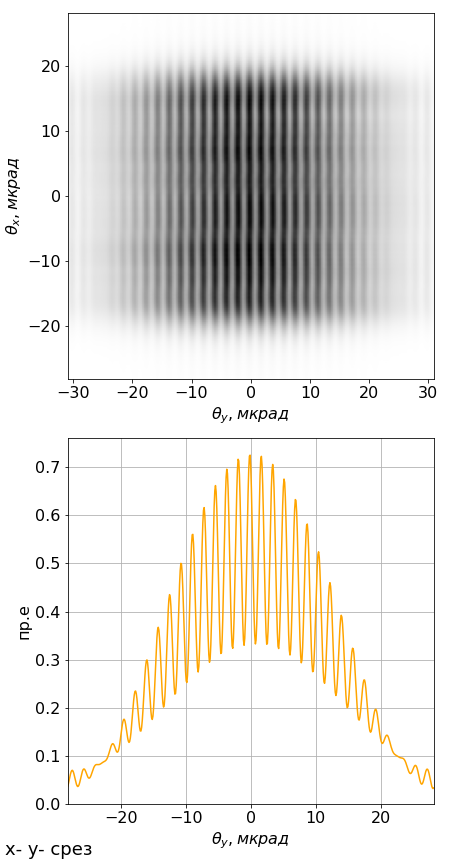
\includegraphics[width=1\linewidth]{y_slits_width_3e-05_separation_0.0003_.png}
		\caption{$300$ мкм}
		\label{fig:y_slits_300}
\end{minipage}\hfill
\end{figure}
Итак, в этом разделе показано влияние частичной когерентности излучения на формирование дифракционной картины. При частично когерентном освещении дифракционная картина «сглаживается»~\cite{goodman_statistical_2015} при уменьшении пятна когерентности или изменение характерного размера оптического элемента, в данном случае межщелевое расстояние. 

\section{Отражение от неидеального зеркала}
В этом разделе мы рассмотрим эффекты возникающие при отражении частично когерентного излучения зеркал с шероховатостями. При отражении от неидеального зеркала волновой фронт деформируется, что, при некачественной полировки поверхности, может в значительной степени влиять на размер и максимальную интенсивность излучения в фокусе, а также на когерентные свойства излучения. Ошибки по высоте $\delta h$ вносят фазовый сдвиг: 
\begin{align}
	\phi = \cfrac{4 \pi \delta h}{\lambda} \sin{(\theta_i)},
	\label{eq:roughness}
\end{align}
где $\theta_i$ -- скользящий угол на зеркало, отсчитываемый от поверхности зеркала. 

Формула~\ref{eq:roughness} даёт простой путь учёта шероховатости поверхностей при моделировании в волновом подходе, таким образом действие неидеальной поверхности учитывается как фазовый фактор, модулирующий волновой фронт. Альтернативный подход -- использование пошагового моделирования процесса отражения волнового фронта от поверхности зеркала с учётом прохождения излучения в вещество, так называемый split-step method~\cite{serkez_design_2015}. Сравнительный анализ этих двух походов приведён в работе~\cite{serkez_design_2015}, где показано совпадение оценки числа Штреля для различных значений среднеквадратического отклонения профиля зеркала, относительно идеальной поверхности. Число Штреля, описывающее относительное падение интенсивности излучения из-за наличия в оптической системе аберраций, может быть использовано для выдвижения критерия (критерий Марешаля) налагающий ограничение на среднеквадратического отклонение $h_{rms}$, а так же отклонение наклона $\mu_{rms}$~\cite{church_specification_1993}:
\begin{align}
	\cfrac{I(0)}{I_0(0)} = 1 - 8\cfrac{\mu^2_{rms}}{\theta_i} - \bigg(\cfrac{4 \pi}{\lambda} \sin{(\theta_i)} \bigg)^2 h^2_{rms} < 0,8.
	\label{eq:Marechal_criterion}
\end{align}
Здесь $I(0)$ и $I_0(0)$ интенсивность излучения на оптической оси в фокусе при отражении от неидеального зеркала и, соответственно, при отражении от идеального зеркала. 

Как видно, формула~\ref{eq:Marechal_criterion} зависит от двух параметров $h_{rms}$ и $\mu_{rms}$. Однако, обычно поверхность зеркала описывается в обратном пространстве частот -- $k$, функцией спектральной плотности $PSD(k)$ по сути являющейся Фурье преобразование профиля зеркала: 
\begin{align}
	PSD(k) =  \cfrac{1}{L} \bigg| \int_{-L/2}^{L/2} \delta h(z) \exp{(-ikz)dz}  \bigg|^2
	\label{eq:PSD_def}
\end{align}
В показано~\cite{angeisky_fractal_nodate}, профиль зеркала имеет фрактальную структуру с параметром D удовлетворяющим $1 < D < 2$, что, соответственно, даёт линейный вид $PSD$-функции в лог-лог масштабе, описываемый двумя параметрами $\alpha$ и $\beta$, при $D = (5 - \alpha)/2$. Соответственно, 
\begin{align}
	\log_{10}(PSD(k)) =  \beta \log_{10}(k) - \alpha.
\end{align}
Через $PSD$-функцию удобно определять среднеквадратичные значения ошибок по высоте и наклону через интегралы:
\begin{align}
	\mu^2_{rms} =  (2 \pi)^2 \int^{1/W}_{1/L} k^2 PSD(k) dk,
\end{align}

\begin{align}
	h^2_{rms} =  \int^{1/\lambda}_{1/W} PSD(k) dk,
\end{align}
где $W$ длина когерентности излучения на зеркале. Видно, что при некоторых значениях $W$ и параметрах оптической системы величина $\mu_{rms}$ теряет свой смысл и равна нулю. Например, для дифракционно ограниченных систем, когда $\theta_{diff} = 1.22 \lambda / D$ много больше чем видимый размер источника $\theta_{source} = \sigma_{x, y}/z_0$, где $z_0$ расстояние от источника до плоскости наблюдения. В этом случае всегда выполняется $W \sim \sqrt{2} L$, \cite{pardini_effect_2015}, и тогда применима формула $h_{rms} < \lambda / 4 \sqrt{5} \pi \theta_i$, что совпадает с аналогичными формулами у~\cite{serkez_design_2015} и~\cite{heimann_linac_2011}\footnote{$4 \pi \sqrt{5}  \approx 28$ }.

Тем не менее, $h_{rms}$ и $\mu_{rms}$ -- некоторые средние, поэтому через них сложно полно описать профиль зеркала. В идеале, при расчёте оптики необходимо знать саму $PSD$ функцию. Обращая формулу~\ref{eq:PSD_def} восстанавливается профиль зеркала~\cite{hua_using_2013},~\cite{xu_statistical_2012},~\cite{barty_predicting_2009}.
\begin{align}
	\delta h(z) = \cfrac{M}{L} F^{-1} \bigg\{\sqrt{L \cdot PSD(k)} \exp{[i \psi(k)]} \bigg\}(z),
\end{align}
где $F^{-1}{\cdot}(z)$ обратное преобразование фурье, а $M$ -- количество точек вдоль оси $z$, $\psi(k)$ -- случайно сгенерированная фаза удовлетворяющая условию $-\pi < \psi(k) <\pi$. Таким образом, зная профиль зеркала $\delta h(z)$ и используя формулу~\ref{eq:roughness}, можно провести моделирование процесса отражения волнового фронта от неидеального зеркала.

Для моделирование была выбрана та же оптическая схема что и для фокусировки с апертурой в разделе~\ref{section:focusing_system_with_aperture}. Однако, чтобы показать действие неидеального зеркала на свойства излучения, апертура была исключена из рассмотрения. На Рис.~\ref{fig:x_SERVAL_radiaiton_after_reflection_2d_3A} и~\ref{fig:y_SERVAL_radiaiton_after_reflection_2d_3A} представлены распределения излучения после отражения от неидеального фокусирующего зеркала со средним значением $h_{rms} = 0,3$ нм и после пропагации волнового фронта через $12,5$ м пустого пространства.
\begin{figure}[H]
	\centering
	\begin{minipage}{0.49\textwidth}
		\centering
		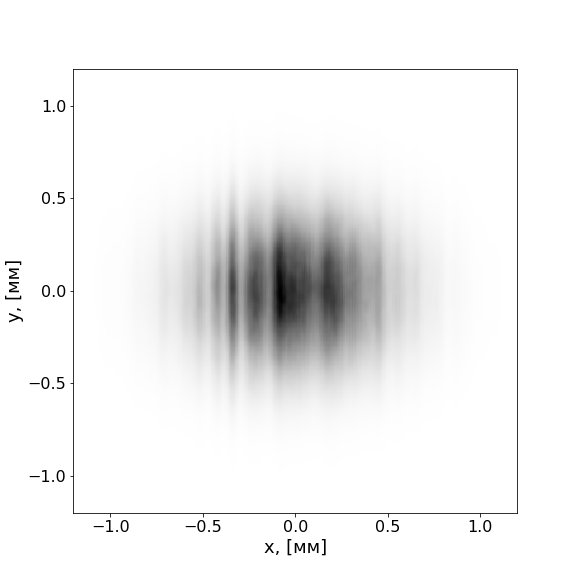
\includegraphics[width=1\linewidth]{x_SERVAL_radiaiton_after_reflection_2d_3.0_A.png}
		\caption{Распределение интенсивности излучения после отражения и $12,5$ м пустого пространства, ошибки по высоте введены по $x$}
		\label{fig:x_SERVAL_radiaiton_after_reflection_2d_3A}
	\end{minipage}
	\begin{minipage}{0.49\textwidth}
		\centering
		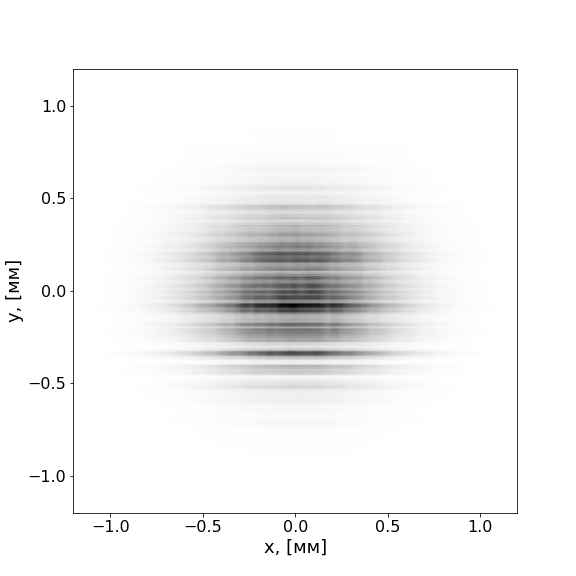
\includegraphics[width=1\linewidth]{y_SERVAL_radiaiton_after_reflection_2d_3.0_A.png}
		\caption{Распределение интенсивности излучения после отражения и $12,5$ м пустого пространства, ошибки по высоте введены по $y$}
		\label{fig:y_SERVAL_radiaiton_after_reflection_2d_3A}
	\end{minipage}\hfill
\end{figure}
\noindent Видно, для горизонтального направление модуляции волнового фронта более сглажены из-за меньшей степени когерентности в этом направлении, в отличии от вертикального направления с большей степенью когерентности.

Для сравнения того, как влияют разные профили зеркала на свойства излучения после пропагации и в фокусе на Рис.~\ref{fig:x_SERVAL_radiaiton_after_reflection},~\ref{fig:y_SERVAL_radiaiton_after_reflection},~\ref{fig:x_SERVAL_radiaiton_in_focus},~\ref{fig:y_SERVAL_radiaiton_in_focus} представлены соответствующие распределения интенсивность излучения после отражения от зеркала со среднеквадратичным отклонениями равными $0,3$ нм и $0,6$ нм. Сравнение приведено для \textit{двух ориентаций} моделируемого зеркала: ошибки введены по горизонтальному направлению  на Рис.~\ref{fig:x_SERVAL_radiaiton_after_reflection},~\ref{fig:x_SERVAL_radiaiton_in_focus}. и, соответственно, по вертикальному направлению на Рис.~\ref{fig:y_SERVAL_radiaiton_after_reflection},~\ref{fig:y_SERVAL_radiaiton_in_focus}, что соответствует вертикальному и горизонтальному ориентациям зеркал. Для всех случаев была выбрана $PSD$ функция с коэффициентом $\beta = -1,8$, нормированная на соответствующие значение среднеквадратического отклонения.

\begin{figure}[H] 
	\centering 	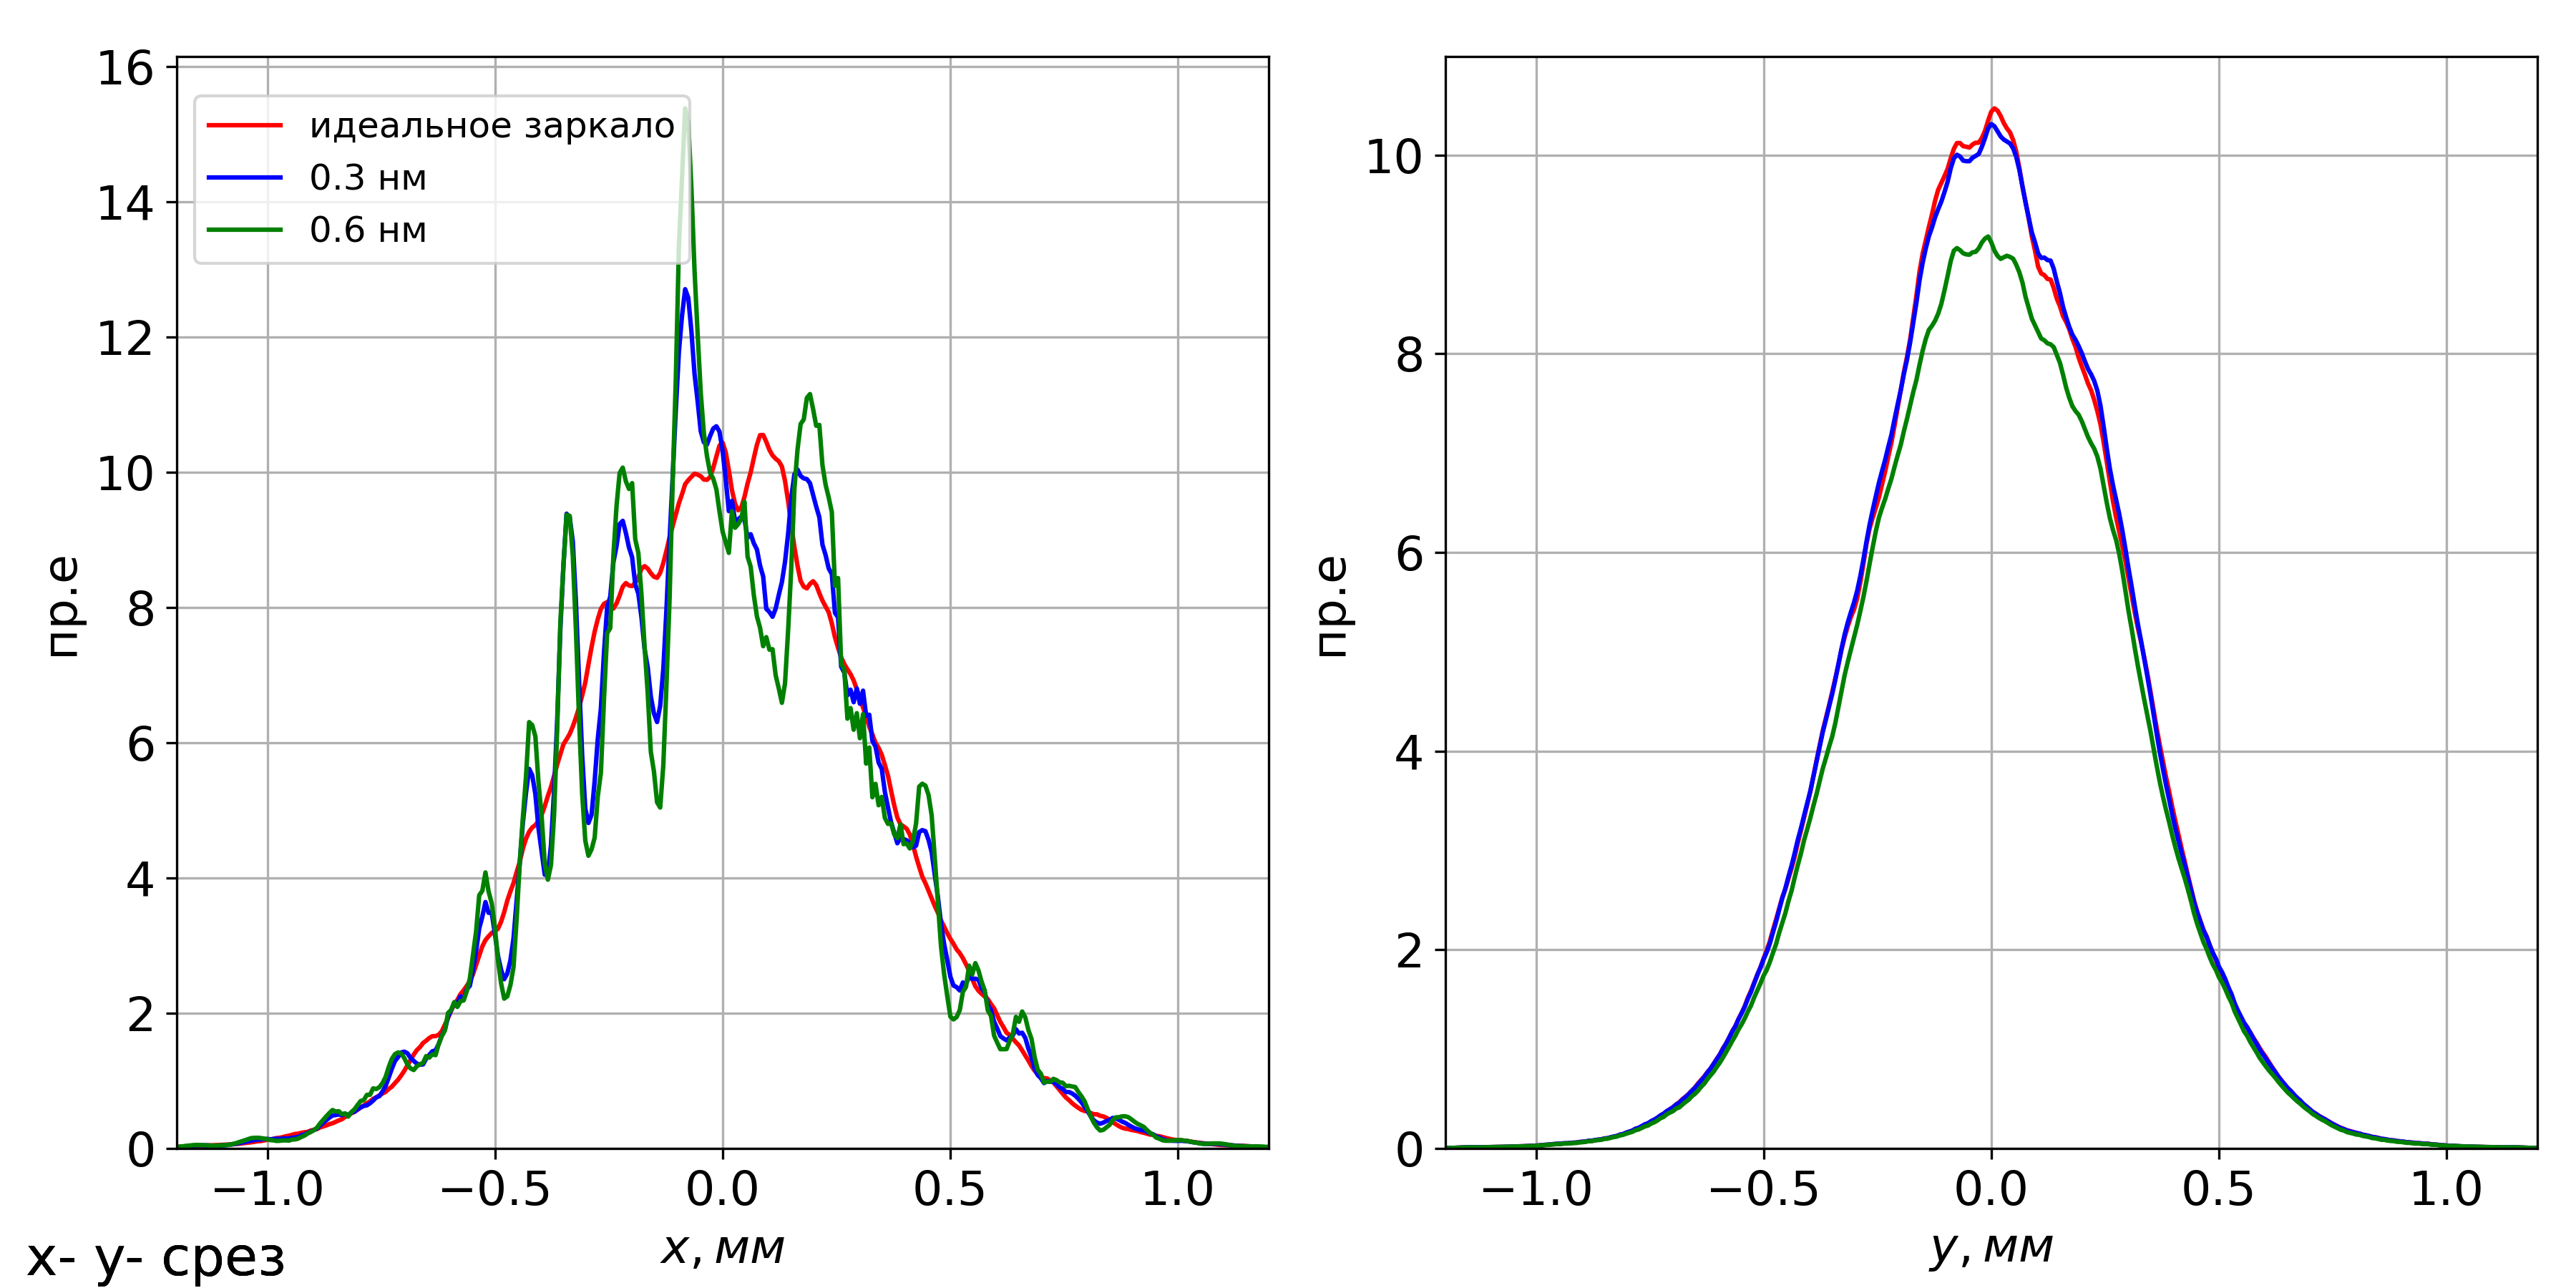
\includegraphics[width=0.99\linewidth]{x_SERVAL_radiaiton_after_reflection.png}
	\caption{Распределение интенсивности излучения после пропагции на 12.5 от зеркала, ошибки по высоте введены по горизонтальному направлению}
	\label{fig:x_SERVAL_radiaiton_after_reflection}
\end{figure}

\begin{figure}[H] 
	\centering 	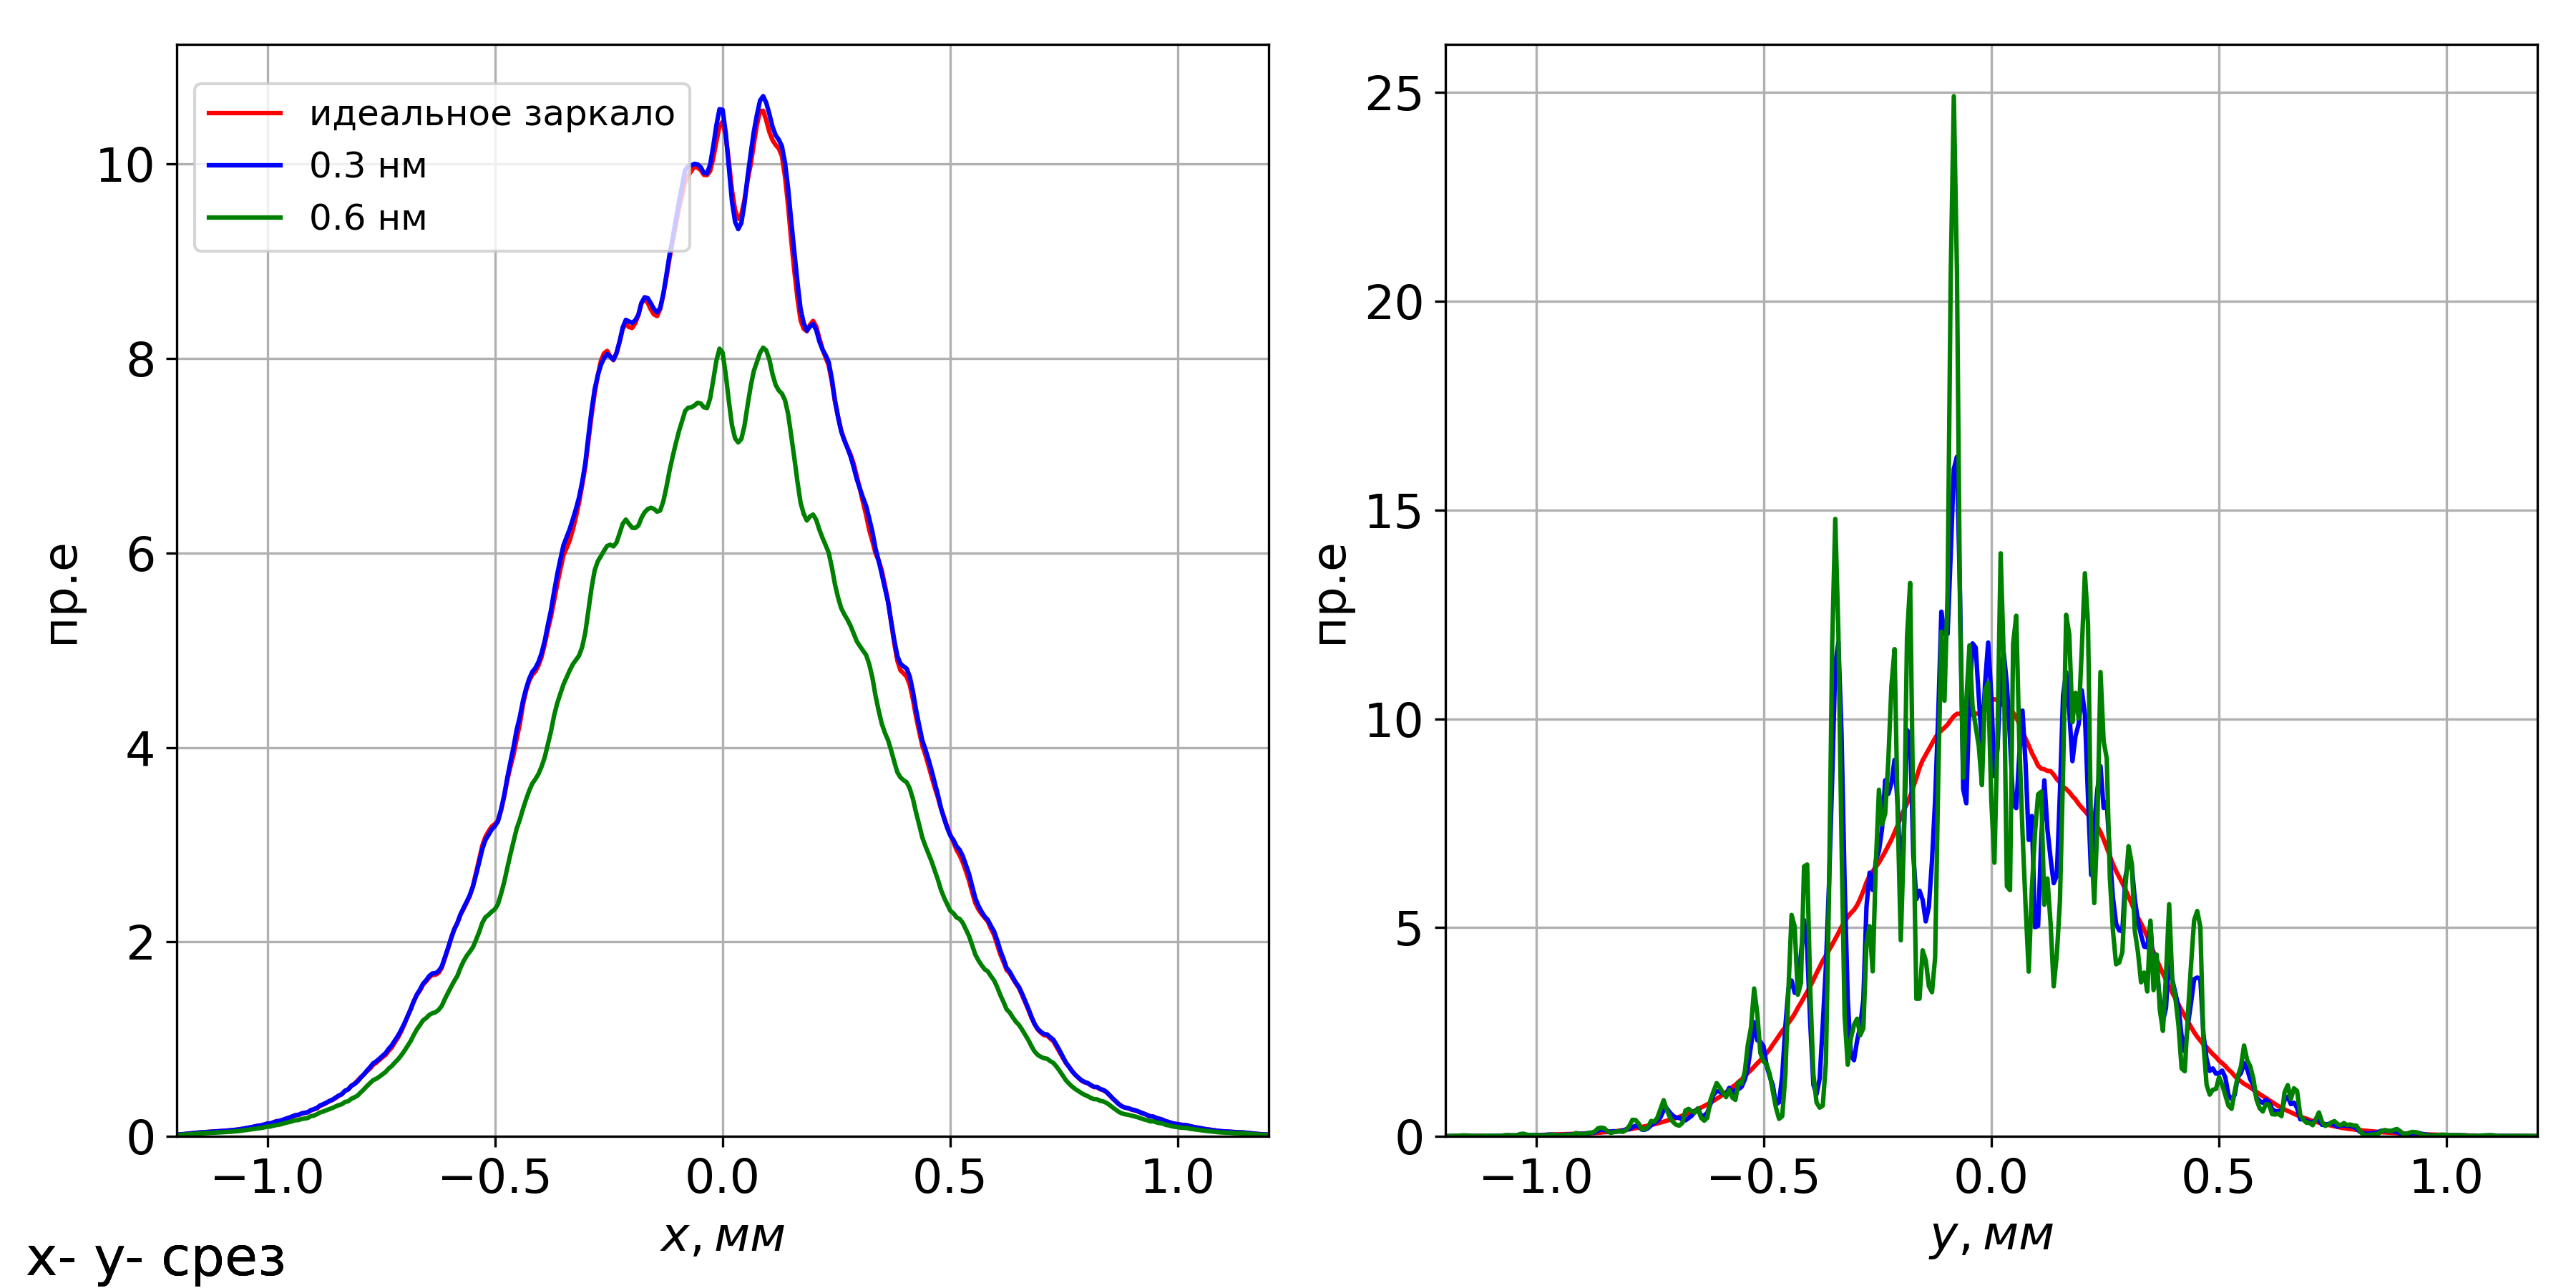
\includegraphics[width=0.99\linewidth]{y_SERVAL_radiaiton_after_reflection.png}
	\caption{Распределение интенсивности излучения после пропагции на 12.5 от зеркала, ошибки по высоте введены по вертикальному направлению}
	\label{fig:y_SERVAL_radiaiton_after_reflection}
\end{figure}
Для каждого из случаев при генерации выбиралось одинаковое начальное число (англ. seed) при генерации псевдослучайного величины, что делалось для воспроизводимости результатов. Именно поэтому модуляции волнового фронта при увеличении величины шероховатости просто повторяют свою форму, но с большей амплитудой.
\begin{figure}[H] 
	\centering 	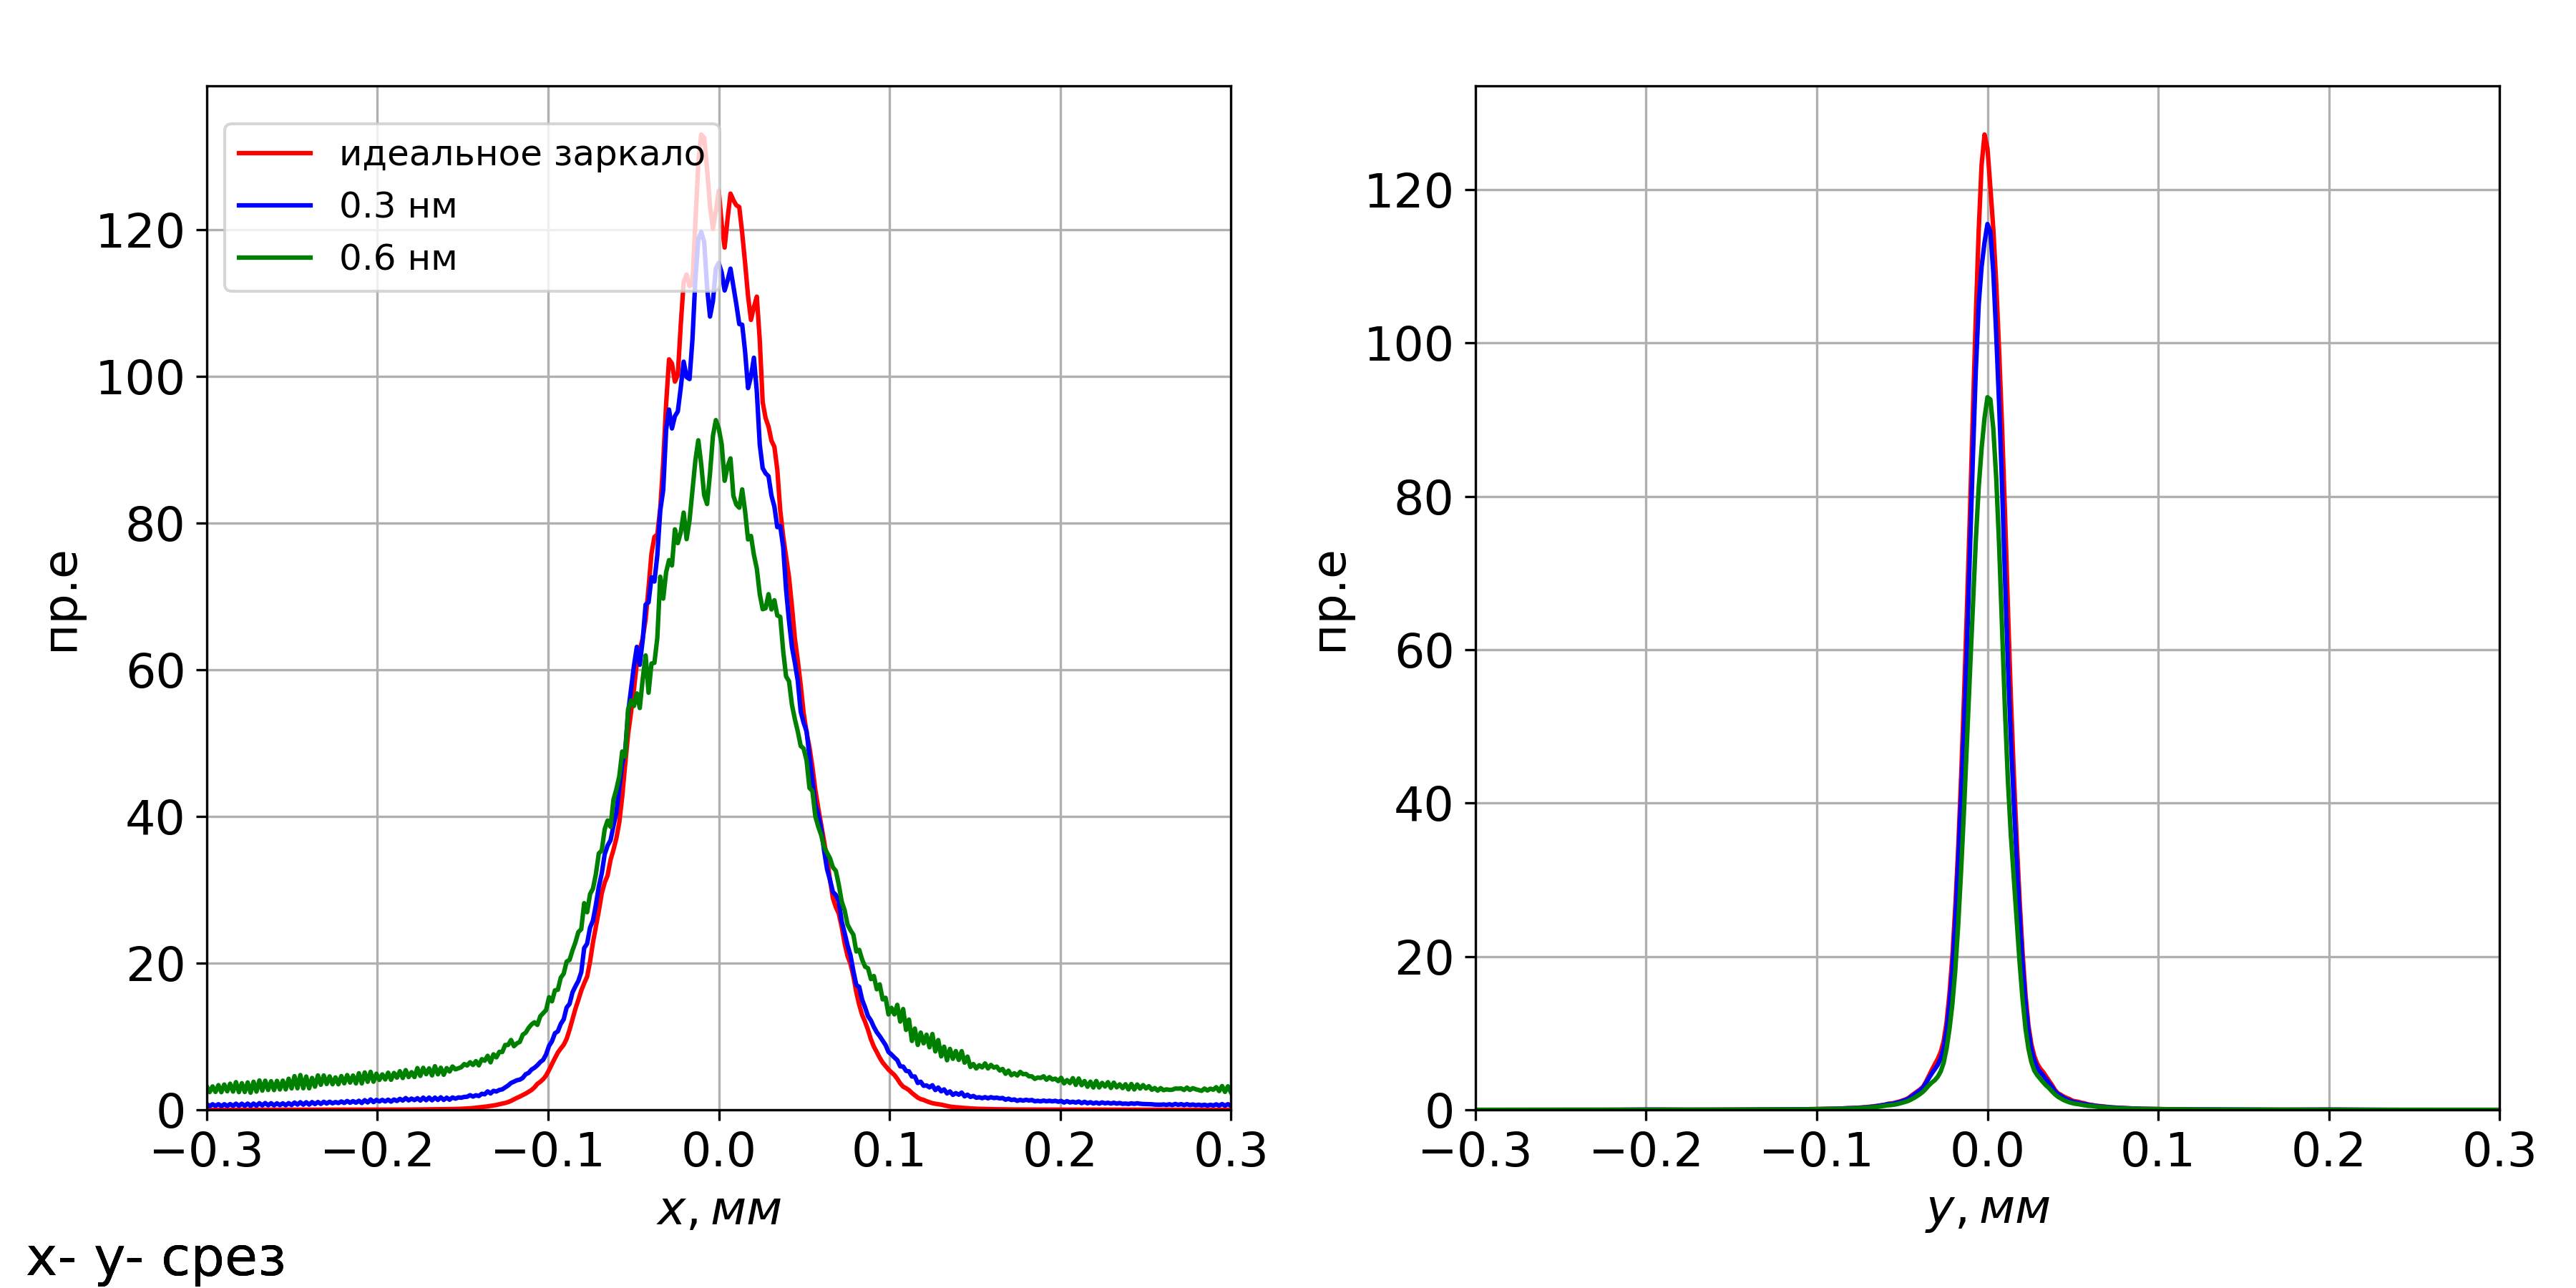
\includegraphics[width=0.99\linewidth]{x_SERVAL_radiaiton_in_focus.png}
	\caption{Распределение интенсивности излучения в фокусе, ошибки по высоте введены по горизонтальному направлению}
	\label{fig:x_SERVAL_radiaiton_in_focus}
\end{figure}

\begin{figure}[H] 
	\centering 	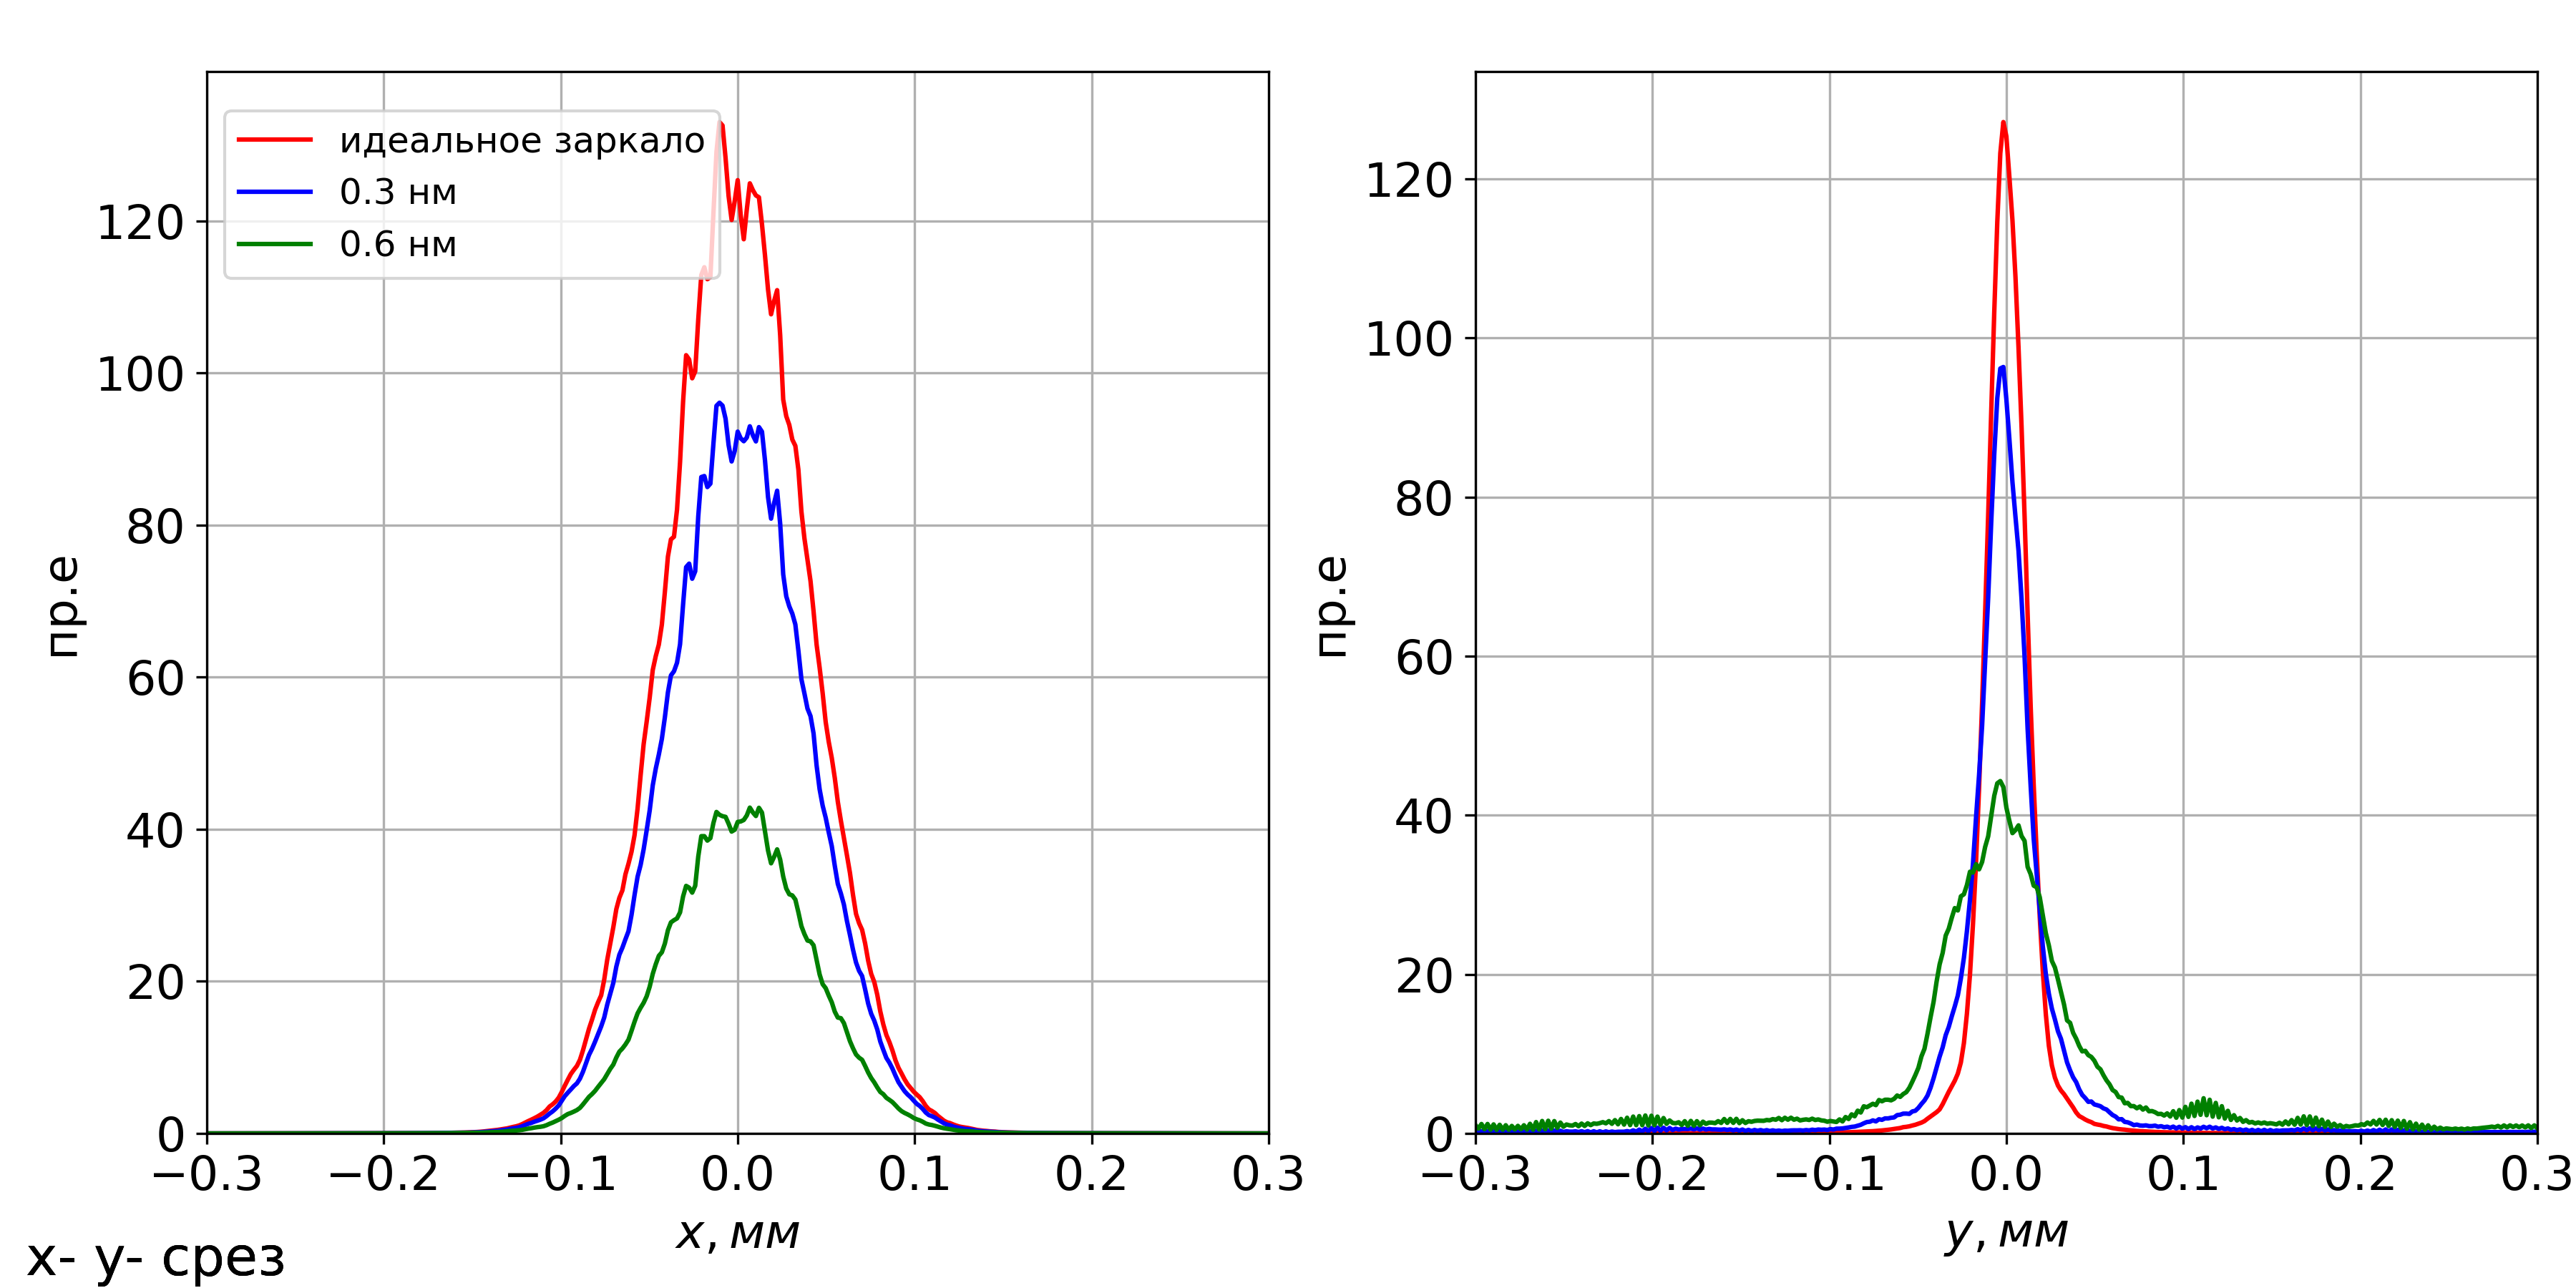
\includegraphics[width=0.99\linewidth]{y_SERVAL_radiaiton_in_focus.png}
	\caption{Распределение интенсивности излучения в фокусе, ошибки по высоте введены по вертикальному направлению}
	\label{fig:y_SERVAL_radiaiton_in_focus}
\end{figure}

Как видно на Рис.~\ref{fig:x_SERVAL_radiaiton_in_focus} и~\ref{fig:y_SERVAL_radiaiton_in_focus} шероховатости приводят к расплыванию фокусного пятна и, следственно, падению пиковой амплитуды интенсивности поля. Например, эффект увеличение размера фокусного пятна приводит к ухудшению разрешающей способности монохроматоров, основанных на дифракционных решётках, поэтому следует налагать довольно жёсткие требования на среднеквадратичную амплитуду шероховатостей рентгеновских зеркал,~\cite{strocov_high-resolution_2010},~\cite{sankari_hippie_nodate}. 

           % Глава 2
%\chapter{Корреляционный анализ модовой структуры} \label{chapt3}



\newpage
%============================================================================================================================

\clearpage           % Глава 3
\chapter*{Заключение}						% Заголовок
%\addcontentsline{toc}{chapter}{Заключение}	% Добавляем его в оглавление

%% Согласно ГОСТ Р 7.0.11-2011:
%% 5.3.3 В заключении диссертации излагают итоги выполненного исследования, рекомендации, перспективы дальнейшей разработки темы.
%% 9.2.3 В заключении автореферата диссертации излагают итоги данного исследования, рекомендации и перспективы дальнейшей разработки темы.
%% Поэтому имеет смысл сделать эту часть общей и загрузить из одного файла в автореферат и в диссертацию:

\rr{Основные результаты работы заключаются в следующем...}
%%% Согласно ГОСТ Р 7.0.11-2011:
%% 5.3.3 В заключении диссертации излагают итоги выполненного исследования, рекомендации, перспективы дальнейшей разработки темы.
%% 9.2.3 В заключении автореферата диссертации излагают итоги данного исследования, рекомендации и перспективы дальнейшей разработки темы.
\begin{enumerate}
  \item Были выработаны оптимальные критерии отбора событий процесса ${e^+\:e^- \to K_{S}\:K_{L}\:\pi^0}$. Вклад данного процесса в общее адронное сечение менее 5\%, тем не менее удалось набрать статистику в 1924 событий при помощи выбора оптимальных условий отбора.
  \item Определена эффективность регистрации при помощи Монте-Карло моделирования, которая составила около 2\% в диапозоне энергий от \text{1.1 ГэВ} до \text{1.4 ГэВ} и около 4.5\% для энергий от 1.4 ГэВ до 2 ГэВ со статистической ошибкой $\sim1\%$.
  \item Измерено сечение процесса ${e^+\:e^- \to K_{S}\:K_{L}\:\pi^0}$ в диапозоне энергий от \text{1.1 ГэВ} до \text{2 ГэВ} со статистической погрешностью около 10\%. Вычислены радиационные поправки с точностью $\sim1\%$, с последующим получением конечного результата --- борновское сечение изучаемого процесса.
  \item Сделана оценка вклада трех основных фоновых событий, общий вклад которых составил не более 10\% от сечения процесса ${e^+\:e^- \to K_{S}\:K_{L}\:\pi^0}$.
\end{enumerate}

      % Заключение
\clearpage                                  % В том числе гарантирует, что список литературы в оглавлении будет с \clearpage                                  % В том числе гарантирует, что список литературы в оглавлении будет с правильным номером страницы
\phantomsection
\addcontentsline{toc}{chapter}{\bibname}	% Добавляем список литературы в оглавление
\hypersetup{ urlcolor=black }               % Ссылки делаем чёрными
%\providecommand*{\BibDash}{}                % В стилях ugost2008 отключаем использование тире как разделителя 
\urlstyle{rm}                               % ссылки URL обычным шрифтом
\insertbiblioother                          % Подключаем Bib-базы
%\insertbibliofull
\urlstyle{tt}                               % возвращаем установки шрифта ссылок URL
%\hypersetup{ urlcolor={urlcolor} }          % Восстанавливаем цвет ссылок      % Список литературы
%\chapter*{Глоссарий}\label{glossarium}
\addcontentsline{toc}{chapter}{Глоссарий}	% Добавляем его в оглавление

\noindent \underline{Эмиттанс} релятивистского электронного пучка -- площадь фазового пространства в $x$, $x'$, $y$, $y'$ поперечных координатах, в работе не рассматривается понятие эмиттанса как объём шестимерного фазового пространства.

\noindent \underline{Пропагация} излучения -- распространение волнового фронта  вдоль оптической оси  от плоскость с позицией $z_1$ до позиции $z_2$.

\noindent \underline{$\text{Si}(\cdot)$} -- интегральный синус.

\noindent \underline{Комплексный гауссов шум} -- статистический процесс описываемы комплексным нормальным распределением: $Z = X + iY$, где $X$ и $Y$ нормальные распределения со средним $0$ и вариацией равной единице. В работе под комплексным гауссовым шумом подразумевается двумерный (или трехмерный) массив величин, где значение каждого элемента является комплексная случайная величина $Z$.

\noindent \underline{SERVAL} -- хищное млекопитающее семейства кошачьих, в работе используется как условное название для наименования предложенного метода моделирование частично когерентного поля ограничением пространственных гармоник комплексного гауссового шума огибающими поля. 

\noindent \underline{Макроэлектрон} -- понятие используемое при моделировании излучения электронного пучка, так как количество электронов в реальном электронном пучке велико и зачастую нет возможности моделировать на компьютере отдельно, приходится разбивать электронный пучок на кластеры -- макроэлектроны, число которых возможно моделировать на обычном персональном компьютере.

\noindent \underline{Метод сложения амплитуд} -- метод для расчёта излучения электронного пучка с конечным эмиттансом, основанный на сложении полей каждого макроэлектрона с последующим усреднением по статистическим реализациям.

\noindent \underline{Метод SRW}

\noindent \underline{Cпайковая структура синхротронного излучения}

\noindent \underline{SASE2}


\newpage
%============================================================================================================================
      % Список литературы
\clearpage
\phantomsection
\addcontentsline{toc}{chapter}{\listfigurename}
\listoffigures									% Список изображений


%%% Список таблиц %%%
% (ГОСТ Р 7.0.11-2011, 5.3.10)
\clearpage
\phantomsection
\addcontentsline{toc}{chapter}{\listtablename}
\listoftables									% Список таблиц
\newpage           % Списки таблиц и изображений (иллюстративный материал)
\appendix
%% Правка оформления ссылок на приложения:
%http://tex.stackexchange.com/questions/56839/chaptername-is-used-even-for-appendix-chapters-in-toc
%http://tex.stackexchange.com/questions/59349/table-of-contents-with-chapter-and-appendix
%% требует двойной компиляции
\addtocontents{toc}{\def\protect\cftchappresnum{\appendixname{} }%
\setlength{\cftchapnumwidth}{\widthof{\cftchapfont\appendixname~Ш\cftchapaftersnum}}%
}
%% Оформление заголовков приложений ближе к ГОСТ:
\sectionformat{\chapter}[display]{% Параметры заголовков разделов в тексте
    label=\chaptertitlename\ \thechapter,% (ГОСТ Р 2.105, 4.3.6)
    labelsep=20pt,
}
\renewcommand\thechapter{\Asbuk{chapter}} % Чтобы приложения русскими буквами нумеровались
\chapter{Анализ подходящих огибающих для СЕРВАЛа} \label{AppendixA}
\rr{В этом Приложении будут более подобно рассмотрены подходящие огибающие для СЕРВАЛа при различных параметрах электронного пучка}
\chapter{Описание шероховатости поверхностей зеркал} \label{AppendixB}
Число Штреля, упомянутое части~\ref{section:roughness}, описывает относительное падение интенсивности излучения на оси из-за наличия в оптической системе аберраций и может быть использовано для выдвижения критерия (критерий Марешаля), налагающего ограничение на среднеквадратичное отклонение $h_{rms}$, а так же ошибку наклона $\mu_{rms}$,~\cite{church_specification_1993}:
\begin{align}
	\cfrac{I(0)}{I_0(0)} = 1 - 8\cfrac{\mu^2_{rms}}{\theta_i} - \bigg(\cfrac{4 \pi}{\lambda} \sin{(\theta_i)} \bigg)^2 h^2_{rms} < 0,8.
	\label{eq:Marechal_criterion}
\end{align}
Здесь $I(0)$ и $I_0(0)$ интенсивность излучения на оптической оси в фокусе при отражении от неидеального зеркала. 

Как видно, формула~\ref{eq:Marechal_criterion} зависит от двух параметров $h_{rms}$ и $\mu_{rms}$. Полное описание поверхности зеркала возможно в обратном пространстве функцией спектральной плотности $PSD(k)$, которая определяется следующим образом: 
\begin{align}
	PSD(k) =  \cfrac{1}{L} \bigg| \int_{-L/2}^{L/2} \delta h(z) \exp{(-ikz)dz}  \bigg|^2
	\label{eq:PSD_def}
\end{align}
В показано~\cite{angeisky_fractal_nodate}, что профиль зеркала имеет фрактальную структуру с параметром $D$, удовлетворяющий условию $1 < D < 2$, что даёт линейный вид $PSD$-функции в лог-лог масштабе, описываемый двумя параметрами: свободным членом $\alpha$ и наклоном $\beta$, при $D = (5 - \alpha)/2$. Соответственно, 
\begin{align}
	PSD_{лог}(k) =  \beta k - \alpha.
\end{align}
Через $PSD$-функцию удобно определять среднеквадратичные значения ошибок по высоте и наклону через интегралы по $PSD$ функции:
\begin{align}
	\mu^2_{rms} =  (2 \pi)^2 \int^{1/W}_{1/L} k^2 PSD(k) dk,
\end{align}

\begin{align}
	h^2_{rms} =  \int^{1/\lambda}_{1/W} PSD(k) dk,
\end{align}
где $W$ длина когерентности излучения на зеркале. Видно, что при некоторых значениях $W$ и параметрах оптической системы, величина $\mu_{rms}$ теряет свой смысл и равна нулю. 
%Например, для дифракционно ограниченных систем, когда $\theta_{diff} = 1.22 \lambda / D$ много больше чем видимый размер источника $\theta_{source} = \sigma_{x, y}/z_0$, где $z_0$ расстояние от источника до плоскости наблюдения. В этом случае всегда выполняется $W \sim \sqrt{2} L$, \cite{pardini_effect_2015}, и тогда применима формула $h_{rms} < \lambda / 4 \sqrt{5} \pi \theta_i$, что совпадает с аналогичными формулами у~\cite{serkez_design_2015} и~\cite{heimann_linac_2011}\footnote{$4 \pi \sqrt{5}  \approx 28$ }.

$h_{rms}$ и $\mu_{rms}$ -- некоторые средние, поэтому через них сложно полно описать профиль зеркала. При расчёте оптики необходимо знать саму $PSD$ функцию. 

Зная PSD функцию зеркала, можно, обращая формулу~\ref{eq:PSD_def}, моделировать профиль зеркала~\cite{hua_using_2013},~\cite{xu_statistical_2012},~\cite{barty_predicting_2009}.
\begin{align}
	\delta h(z) = \cfrac{M}{L} F^{-1} \bigg\{\sqrt{L \cdot PSD(k)} \exp{[i \psi(k)]} \bigg\}(z),
\end{align}
где $F^{-1}\{\cdot\}(z)$ обратное преобразование фурье, а $M$ -- количество точек вдоль оси $z$, $\psi(k)$ -- случайно сгенерированная фаза, удовлетворяющая условию $-\pi < \psi(k) <\pi$, равномерно распределенная в этом промежутке. Таким образом, зная профиль зеркала $\delta h(z)$ и используя формулу~\ref{eq:roughness}, можно провести моделирование процесса отражения волнового фронта от неидеального зеркала.
\normalsize% возвращаем шрифт к нормальному
        % Приложения

\end{document}
